\documentclass[11pt]{article}

    \usepackage[breakable]{tcolorbox}
    \usepackage{parskip} % Stop auto-indenting (to mimic markdown behaviour)
    

    % Basic figure setup, for now with no caption control since it's done
    % automatically by Pandoc (which extracts ![](path) syntax from Markdown).
    \usepackage{graphicx}
    % Keep aspect ratio if custom image width or height is specified
    \setkeys{Gin}{keepaspectratio}
    % Maintain compatibility with old templates. Remove in nbconvert 6.0
    \let\Oldincludegraphics\includegraphics
    % Ensure that by default, figures have no caption (until we provide a
    % proper Figure object with a Caption API and a way to capture that
    % in the conversion process - todo).
    \usepackage{caption}
    \DeclareCaptionFormat{nocaption}{}
    \captionsetup{format=nocaption,aboveskip=0pt,belowskip=0pt}

    \usepackage{float}
    \floatplacement{figure}{H} % forces figures to be placed at the correct location
    \usepackage{xcolor} % Allow colors to be defined
    \usepackage{enumerate} % Needed for markdown enumerations to work
    \usepackage{geometry} % Used to adjust the document margins
    \usepackage{amsmath} % Equations
    \usepackage{amssymb} % Equations
    \usepackage{textcomp} % defines textquotesingle
    % Hack from http://tex.stackexchange.com/a/47451/13684:
    \AtBeginDocument{%
        \def\PYZsq{\textquotesingle}% Upright quotes in Pygmentized code
    }
    \usepackage{upquote} % Upright quotes for verbatim code
    \usepackage{eurosym} % defines \euro

    \usepackage{iftex}
    \ifPDFTeX
        \usepackage[T1]{fontenc}
        \IfFileExists{alphabeta.sty}{
              \usepackage{alphabeta}
          }{
              \usepackage[mathletters]{ucs}
              \usepackage[utf8x]{inputenc}
          }
    \else
        \usepackage{fontspec}
        \usepackage{unicode-math}
    \fi

    \usepackage{fancyvrb} % verbatim replacement that allows latex
    \usepackage{grffile} % extends the file name processing of package graphics
                         % to support a larger range
    \makeatletter % fix for old versions of grffile with XeLaTeX
    \@ifpackagelater{grffile}{2019/11/01}
    {
      % Do nothing on new versions
    }
    {
      \def\Gread@@xetex#1{%
        \IfFileExists{"\Gin@base".bb}%
        {\Gread@eps{\Gin@base.bb}}%
        {\Gread@@xetex@aux#1}%
      }
    }
    \makeatother
    \usepackage[Export]{adjustbox} % Used to constrain images to a maximum size
    \adjustboxset{max size={0.9\linewidth}{0.9\paperheight}}

    % The hyperref package gives us a pdf with properly built
    % internal navigation ('pdf bookmarks' for the table of contents,
    % internal cross-reference links, web links for URLs, etc.)
    \usepackage{hyperref}
    % The default LaTeX title has an obnoxious amount of whitespace. By default,
    % titling removes some of it. It also provides customization options.
    \usepackage{titling}
    \usepackage{longtable} % longtable support required by pandoc >1.10
    \usepackage{booktabs}  % table support for pandoc > 1.12.2
    \usepackage{array}     % table support for pandoc >= 2.11.3
    \usepackage{calc}      % table minipage width calculation for pandoc >= 2.11.1
    \usepackage[inline]{enumitem} % IRkernel/repr support (it uses the enumerate* environment)
    \usepackage[normalem]{ulem} % ulem is needed to support strikethroughs (\sout)
                                % normalem makes italics be italics, not underlines
    \usepackage{soul}      % strikethrough (\st) support for pandoc >= 3.0.0
    \usepackage{mathrsfs}
    

    
    % Colors for the hyperref package
    \definecolor{urlcolor}{rgb}{0,.145,.698}
    \definecolor{linkcolor}{rgb}{.71,0.21,0.01}
    \definecolor{citecolor}{rgb}{.12,.54,.11}

    % ANSI colors
    \definecolor{ansi-black}{HTML}{3E424D}
    \definecolor{ansi-black-intense}{HTML}{282C36}
    \definecolor{ansi-red}{HTML}{E75C58}
    \definecolor{ansi-red-intense}{HTML}{B22B31}
    \definecolor{ansi-green}{HTML}{00A250}
    \definecolor{ansi-green-intense}{HTML}{007427}
    \definecolor{ansi-yellow}{HTML}{DDB62B}
    \definecolor{ansi-yellow-intense}{HTML}{B27D12}
    \definecolor{ansi-blue}{HTML}{208FFB}
    \definecolor{ansi-blue-intense}{HTML}{0065CA}
    \definecolor{ansi-magenta}{HTML}{D160C4}
    \definecolor{ansi-magenta-intense}{HTML}{A03196}
    \definecolor{ansi-cyan}{HTML}{60C6C8}
    \definecolor{ansi-cyan-intense}{HTML}{258F8F}
    \definecolor{ansi-white}{HTML}{C5C1B4}
    \definecolor{ansi-white-intense}{HTML}{A1A6B2}
    \definecolor{ansi-default-inverse-fg}{HTML}{FFFFFF}
    \definecolor{ansi-default-inverse-bg}{HTML}{000000}

    % common color for the border for error outputs.
    \definecolor{outerrorbackground}{HTML}{FFDFDF}

    % commands and environments needed by pandoc snippets
    % extracted from the output of `pandoc -s`
    \providecommand{\tightlist}{%
      \setlength{\itemsep}{0pt}\setlength{\parskip}{0pt}}
    \DefineVerbatimEnvironment{Highlighting}{Verbatim}{commandchars=\\\{\}}
    % Add ',fontsize=\small' for more characters per line
    \newenvironment{Shaded}{}{}
    \newcommand{\KeywordTok}[1]{\textcolor[rgb]{0.00,0.44,0.13}{\textbf{{#1}}}}
    \newcommand{\DataTypeTok}[1]{\textcolor[rgb]{0.56,0.13,0.00}{{#1}}}
    \newcommand{\DecValTok}[1]{\textcolor[rgb]{0.25,0.63,0.44}{{#1}}}
    \newcommand{\BaseNTok}[1]{\textcolor[rgb]{0.25,0.63,0.44}{{#1}}}
    \newcommand{\FloatTok}[1]{\textcolor[rgb]{0.25,0.63,0.44}{{#1}}}
    \newcommand{\CharTok}[1]{\textcolor[rgb]{0.25,0.44,0.63}{{#1}}}
    \newcommand{\StringTok}[1]{\textcolor[rgb]{0.25,0.44,0.63}{{#1}}}
    \newcommand{\CommentTok}[1]{\textcolor[rgb]{0.38,0.63,0.69}{\textit{{#1}}}}
    \newcommand{\OtherTok}[1]{\textcolor[rgb]{0.00,0.44,0.13}{{#1}}}
    \newcommand{\AlertTok}[1]{\textcolor[rgb]{1.00,0.00,0.00}{\textbf{{#1}}}}
    \newcommand{\FunctionTok}[1]{\textcolor[rgb]{0.02,0.16,0.49}{{#1}}}
    \newcommand{\RegionMarkerTok}[1]{{#1}}
    \newcommand{\ErrorTok}[1]{\textcolor[rgb]{1.00,0.00,0.00}{\textbf{{#1}}}}
    \newcommand{\NormalTok}[1]{{#1}}

    % Additional commands for more recent versions of Pandoc
    \newcommand{\ConstantTok}[1]{\textcolor[rgb]{0.53,0.00,0.00}{{#1}}}
    \newcommand{\SpecialCharTok}[1]{\textcolor[rgb]{0.25,0.44,0.63}{{#1}}}
    \newcommand{\VerbatimStringTok}[1]{\textcolor[rgb]{0.25,0.44,0.63}{{#1}}}
    \newcommand{\SpecialStringTok}[1]{\textcolor[rgb]{0.73,0.40,0.53}{{#1}}}
    \newcommand{\ImportTok}[1]{{#1}}
    \newcommand{\DocumentationTok}[1]{\textcolor[rgb]{0.73,0.13,0.13}{\textit{{#1}}}}
    \newcommand{\AnnotationTok}[1]{\textcolor[rgb]{0.38,0.63,0.69}{\textbf{\textit{{#1}}}}}
    \newcommand{\CommentVarTok}[1]{\textcolor[rgb]{0.38,0.63,0.69}{\textbf{\textit{{#1}}}}}
    \newcommand{\VariableTok}[1]{\textcolor[rgb]{0.10,0.09,0.49}{{#1}}}
    \newcommand{\ControlFlowTok}[1]{\textcolor[rgb]{0.00,0.44,0.13}{\textbf{{#1}}}}
    \newcommand{\OperatorTok}[1]{\textcolor[rgb]{0.40,0.40,0.40}{{#1}}}
    \newcommand{\BuiltInTok}[1]{{#1}}
    \newcommand{\ExtensionTok}[1]{{#1}}
    \newcommand{\PreprocessorTok}[1]{\textcolor[rgb]{0.74,0.48,0.00}{{#1}}}
    \newcommand{\AttributeTok}[1]{\textcolor[rgb]{0.49,0.56,0.16}{{#1}}}
    \newcommand{\InformationTok}[1]{\textcolor[rgb]{0.38,0.63,0.69}{\textbf{\textit{{#1}}}}}
    \newcommand{\WarningTok}[1]{\textcolor[rgb]{0.38,0.63,0.69}{\textbf{\textit{{#1}}}}}
    \makeatletter
    \newsavebox\pandoc@box
    \newcommand*\pandocbounded[1]{%
      \sbox\pandoc@box{#1}%
      % scaling factors for width and height
      \Gscale@div\@tempa\textheight{\dimexpr\ht\pandoc@box+\dp\pandoc@box\relax}%
      \Gscale@div\@tempb\linewidth{\wd\pandoc@box}%
      % select the smaller of both
      \ifdim\@tempb\p@<\@tempa\p@
        \let\@tempa\@tempb
      \fi
      % scaling accordingly (\@tempa < 1)
      \ifdim\@tempa\p@<\p@
        \scalebox{\@tempa}{\usebox\pandoc@box}%
      % scaling not needed, use as it is
      \else
        \usebox{\pandoc@box}%
      \fi
    }
    \makeatother

    % Define a nice break command that doesn't care if a line doesn't already
    % exist.
    \def\br{\hspace*{\fill} \\* }
    % Math Jax compatibility definitions
    \def\gt{>}
    \def\lt{<}
    \let\Oldtex\TeX
    \let\Oldlatex\LaTeX
    \renewcommand{\TeX}{\textrm{\Oldtex}}
    \renewcommand{\LaTeX}{\textrm{\Oldlatex}}
    % Document parameters
    % Document title
    \title{MDS\_Assignment2\_313652018\_Wang\_Xuan-Wei}
    
    
    
    
    
    
    
% Pygments definitions
\makeatletter
\def\PY@reset{\let\PY@it=\relax \let\PY@bf=\relax%
    \let\PY@ul=\relax \let\PY@tc=\relax%
    \let\PY@bc=\relax \let\PY@ff=\relax}
\def\PY@tok#1{\csname PY@tok@#1\endcsname}
\def\PY@toks#1+{\ifx\relax#1\empty\else%
    \PY@tok{#1}\expandafter\PY@toks\fi}
\def\PY@do#1{\PY@bc{\PY@tc{\PY@ul{%
    \PY@it{\PY@bf{\PY@ff{#1}}}}}}}
\def\PY#1#2{\PY@reset\PY@toks#1+\relax+\PY@do{#2}}

\@namedef{PY@tok@w}{\def\PY@tc##1{\textcolor[rgb]{0.73,0.73,0.73}{##1}}}
\@namedef{PY@tok@c}{\let\PY@it=\textit\def\PY@tc##1{\textcolor[rgb]{0.24,0.48,0.48}{##1}}}
\@namedef{PY@tok@cp}{\def\PY@tc##1{\textcolor[rgb]{0.61,0.40,0.00}{##1}}}
\@namedef{PY@tok@k}{\let\PY@bf=\textbf\def\PY@tc##1{\textcolor[rgb]{0.00,0.50,0.00}{##1}}}
\@namedef{PY@tok@kp}{\def\PY@tc##1{\textcolor[rgb]{0.00,0.50,0.00}{##1}}}
\@namedef{PY@tok@kt}{\def\PY@tc##1{\textcolor[rgb]{0.69,0.00,0.25}{##1}}}
\@namedef{PY@tok@o}{\def\PY@tc##1{\textcolor[rgb]{0.40,0.40,0.40}{##1}}}
\@namedef{PY@tok@ow}{\let\PY@bf=\textbf\def\PY@tc##1{\textcolor[rgb]{0.67,0.13,1.00}{##1}}}
\@namedef{PY@tok@nb}{\def\PY@tc##1{\textcolor[rgb]{0.00,0.50,0.00}{##1}}}
\@namedef{PY@tok@nf}{\def\PY@tc##1{\textcolor[rgb]{0.00,0.00,1.00}{##1}}}
\@namedef{PY@tok@nc}{\let\PY@bf=\textbf\def\PY@tc##1{\textcolor[rgb]{0.00,0.00,1.00}{##1}}}
\@namedef{PY@tok@nn}{\let\PY@bf=\textbf\def\PY@tc##1{\textcolor[rgb]{0.00,0.00,1.00}{##1}}}
\@namedef{PY@tok@ne}{\let\PY@bf=\textbf\def\PY@tc##1{\textcolor[rgb]{0.80,0.25,0.22}{##1}}}
\@namedef{PY@tok@nv}{\def\PY@tc##1{\textcolor[rgb]{0.10,0.09,0.49}{##1}}}
\@namedef{PY@tok@no}{\def\PY@tc##1{\textcolor[rgb]{0.53,0.00,0.00}{##1}}}
\@namedef{PY@tok@nl}{\def\PY@tc##1{\textcolor[rgb]{0.46,0.46,0.00}{##1}}}
\@namedef{PY@tok@ni}{\let\PY@bf=\textbf\def\PY@tc##1{\textcolor[rgb]{0.44,0.44,0.44}{##1}}}
\@namedef{PY@tok@na}{\def\PY@tc##1{\textcolor[rgb]{0.41,0.47,0.13}{##1}}}
\@namedef{PY@tok@nt}{\let\PY@bf=\textbf\def\PY@tc##1{\textcolor[rgb]{0.00,0.50,0.00}{##1}}}
\@namedef{PY@tok@nd}{\def\PY@tc##1{\textcolor[rgb]{0.67,0.13,1.00}{##1}}}
\@namedef{PY@tok@s}{\def\PY@tc##1{\textcolor[rgb]{0.73,0.13,0.13}{##1}}}
\@namedef{PY@tok@sd}{\let\PY@it=\textit\def\PY@tc##1{\textcolor[rgb]{0.73,0.13,0.13}{##1}}}
\@namedef{PY@tok@si}{\let\PY@bf=\textbf\def\PY@tc##1{\textcolor[rgb]{0.64,0.35,0.47}{##1}}}
\@namedef{PY@tok@se}{\let\PY@bf=\textbf\def\PY@tc##1{\textcolor[rgb]{0.67,0.36,0.12}{##1}}}
\@namedef{PY@tok@sr}{\def\PY@tc##1{\textcolor[rgb]{0.64,0.35,0.47}{##1}}}
\@namedef{PY@tok@ss}{\def\PY@tc##1{\textcolor[rgb]{0.10,0.09,0.49}{##1}}}
\@namedef{PY@tok@sx}{\def\PY@tc##1{\textcolor[rgb]{0.00,0.50,0.00}{##1}}}
\@namedef{PY@tok@m}{\def\PY@tc##1{\textcolor[rgb]{0.40,0.40,0.40}{##1}}}
\@namedef{PY@tok@gh}{\let\PY@bf=\textbf\def\PY@tc##1{\textcolor[rgb]{0.00,0.00,0.50}{##1}}}
\@namedef{PY@tok@gu}{\let\PY@bf=\textbf\def\PY@tc##1{\textcolor[rgb]{0.50,0.00,0.50}{##1}}}
\@namedef{PY@tok@gd}{\def\PY@tc##1{\textcolor[rgb]{0.63,0.00,0.00}{##1}}}
\@namedef{PY@tok@gi}{\def\PY@tc##1{\textcolor[rgb]{0.00,0.52,0.00}{##1}}}
\@namedef{PY@tok@gr}{\def\PY@tc##1{\textcolor[rgb]{0.89,0.00,0.00}{##1}}}
\@namedef{PY@tok@ge}{\let\PY@it=\textit}
\@namedef{PY@tok@gs}{\let\PY@bf=\textbf}
\@namedef{PY@tok@ges}{\let\PY@bf=\textbf\let\PY@it=\textit}
\@namedef{PY@tok@gp}{\let\PY@bf=\textbf\def\PY@tc##1{\textcolor[rgb]{0.00,0.00,0.50}{##1}}}
\@namedef{PY@tok@go}{\def\PY@tc##1{\textcolor[rgb]{0.44,0.44,0.44}{##1}}}
\@namedef{PY@tok@gt}{\def\PY@tc##1{\textcolor[rgb]{0.00,0.27,0.87}{##1}}}
\@namedef{PY@tok@err}{\def\PY@bc##1{{\setlength{\fboxsep}{\string -\fboxrule}\fcolorbox[rgb]{1.00,0.00,0.00}{1,1,1}{\strut ##1}}}}
\@namedef{PY@tok@kc}{\let\PY@bf=\textbf\def\PY@tc##1{\textcolor[rgb]{0.00,0.50,0.00}{##1}}}
\@namedef{PY@tok@kd}{\let\PY@bf=\textbf\def\PY@tc##1{\textcolor[rgb]{0.00,0.50,0.00}{##1}}}
\@namedef{PY@tok@kn}{\let\PY@bf=\textbf\def\PY@tc##1{\textcolor[rgb]{0.00,0.50,0.00}{##1}}}
\@namedef{PY@tok@kr}{\let\PY@bf=\textbf\def\PY@tc##1{\textcolor[rgb]{0.00,0.50,0.00}{##1}}}
\@namedef{PY@tok@bp}{\def\PY@tc##1{\textcolor[rgb]{0.00,0.50,0.00}{##1}}}
\@namedef{PY@tok@fm}{\def\PY@tc##1{\textcolor[rgb]{0.00,0.00,1.00}{##1}}}
\@namedef{PY@tok@vc}{\def\PY@tc##1{\textcolor[rgb]{0.10,0.09,0.49}{##1}}}
\@namedef{PY@tok@vg}{\def\PY@tc##1{\textcolor[rgb]{0.10,0.09,0.49}{##1}}}
\@namedef{PY@tok@vi}{\def\PY@tc##1{\textcolor[rgb]{0.10,0.09,0.49}{##1}}}
\@namedef{PY@tok@vm}{\def\PY@tc##1{\textcolor[rgb]{0.10,0.09,0.49}{##1}}}
\@namedef{PY@tok@sa}{\def\PY@tc##1{\textcolor[rgb]{0.73,0.13,0.13}{##1}}}
\@namedef{PY@tok@sb}{\def\PY@tc##1{\textcolor[rgb]{0.73,0.13,0.13}{##1}}}
\@namedef{PY@tok@sc}{\def\PY@tc##1{\textcolor[rgb]{0.73,0.13,0.13}{##1}}}
\@namedef{PY@tok@dl}{\def\PY@tc##1{\textcolor[rgb]{0.73,0.13,0.13}{##1}}}
\@namedef{PY@tok@s2}{\def\PY@tc##1{\textcolor[rgb]{0.73,0.13,0.13}{##1}}}
\@namedef{PY@tok@sh}{\def\PY@tc##1{\textcolor[rgb]{0.73,0.13,0.13}{##1}}}
\@namedef{PY@tok@s1}{\def\PY@tc##1{\textcolor[rgb]{0.73,0.13,0.13}{##1}}}
\@namedef{PY@tok@mb}{\def\PY@tc##1{\textcolor[rgb]{0.40,0.40,0.40}{##1}}}
\@namedef{PY@tok@mf}{\def\PY@tc##1{\textcolor[rgb]{0.40,0.40,0.40}{##1}}}
\@namedef{PY@tok@mh}{\def\PY@tc##1{\textcolor[rgb]{0.40,0.40,0.40}{##1}}}
\@namedef{PY@tok@mi}{\def\PY@tc##1{\textcolor[rgb]{0.40,0.40,0.40}{##1}}}
\@namedef{PY@tok@il}{\def\PY@tc##1{\textcolor[rgb]{0.40,0.40,0.40}{##1}}}
\@namedef{PY@tok@mo}{\def\PY@tc##1{\textcolor[rgb]{0.40,0.40,0.40}{##1}}}
\@namedef{PY@tok@ch}{\let\PY@it=\textit\def\PY@tc##1{\textcolor[rgb]{0.24,0.48,0.48}{##1}}}
\@namedef{PY@tok@cm}{\let\PY@it=\textit\def\PY@tc##1{\textcolor[rgb]{0.24,0.48,0.48}{##1}}}
\@namedef{PY@tok@cpf}{\let\PY@it=\textit\def\PY@tc##1{\textcolor[rgb]{0.24,0.48,0.48}{##1}}}
\@namedef{PY@tok@c1}{\let\PY@it=\textit\def\PY@tc##1{\textcolor[rgb]{0.24,0.48,0.48}{##1}}}
\@namedef{PY@tok@cs}{\let\PY@it=\textit\def\PY@tc##1{\textcolor[rgb]{0.24,0.48,0.48}{##1}}}

\def\PYZbs{\char`\\}
\def\PYZus{\char`\_}
\def\PYZob{\char`\{}
\def\PYZcb{\char`\}}
\def\PYZca{\char`\^}
\def\PYZam{\char`\&}
\def\PYZlt{\char`\<}
\def\PYZgt{\char`\>}
\def\PYZsh{\char`\#}
\def\PYZpc{\char`\%}
\def\PYZdl{\char`\$}
\def\PYZhy{\char`\-}
\def\PYZsq{\char`\'}
\def\PYZdq{\char`\"}
\def\PYZti{\char`\~}
% for compatibility with earlier versions
\def\PYZat{@}
\def\PYZlb{[}
\def\PYZrb{]}
\makeatother


    % For linebreaks inside Verbatim environment from package fancyvrb.
    \makeatletter
        \newbox\Wrappedcontinuationbox
        \newbox\Wrappedvisiblespacebox
        \newcommand*\Wrappedvisiblespace {\textcolor{red}{\textvisiblespace}}
        \newcommand*\Wrappedcontinuationsymbol {\textcolor{red}{\llap{\tiny$\m@th\hookrightarrow$}}}
        \newcommand*\Wrappedcontinuationindent {3ex }
        \newcommand*\Wrappedafterbreak {\kern\Wrappedcontinuationindent\copy\Wrappedcontinuationbox}
        % Take advantage of the already applied Pygments mark-up to insert
        % potential linebreaks for TeX processing.
        %        {, <, #, %, $, ' and ": go to next line.
        %        _, }, ^, &, >, - and ~: stay at end of broken line.
        % Use of \textquotesingle for straight quote.
        \newcommand*\Wrappedbreaksatspecials {%
            \def\PYGZus{\discretionary{\char`\_}{\Wrappedafterbreak}{\char`\_}}%
            \def\PYGZob{\discretionary{}{\Wrappedafterbreak\char`\{}{\char`\{}}%
            \def\PYGZcb{\discretionary{\char`\}}{\Wrappedafterbreak}{\char`\}}}%
            \def\PYGZca{\discretionary{\char`\^}{\Wrappedafterbreak}{\char`\^}}%
            \def\PYGZam{\discretionary{\char`\&}{\Wrappedafterbreak}{\char`\&}}%
            \def\PYGZlt{\discretionary{}{\Wrappedafterbreak\char`\<}{\char`\<}}%
            \def\PYGZgt{\discretionary{\char`\>}{\Wrappedafterbreak}{\char`\>}}%
            \def\PYGZsh{\discretionary{}{\Wrappedafterbreak\char`\#}{\char`\#}}%
            \def\PYGZpc{\discretionary{}{\Wrappedafterbreak\char`\%}{\char`\%}}%
            \def\PYGZdl{\discretionary{}{\Wrappedafterbreak\char`\$}{\char`\$}}%
            \def\PYGZhy{\discretionary{\char`\-}{\Wrappedafterbreak}{\char`\-}}%
            \def\PYGZsq{\discretionary{}{\Wrappedafterbreak\textquotesingle}{\textquotesingle}}%
            \def\PYGZdq{\discretionary{}{\Wrappedafterbreak\char`\"}{\char`\"}}%
            \def\PYGZti{\discretionary{\char`\~}{\Wrappedafterbreak}{\char`\~}}%
        }
        % Some characters . , ; ? ! / are not pygmentized.
        % This macro makes them "active" and they will insert potential linebreaks
        \newcommand*\Wrappedbreaksatpunct {%
            \lccode`\~`\.\lowercase{\def~}{\discretionary{\hbox{\char`\.}}{\Wrappedafterbreak}{\hbox{\char`\.}}}%
            \lccode`\~`\,\lowercase{\def~}{\discretionary{\hbox{\char`\,}}{\Wrappedafterbreak}{\hbox{\char`\,}}}%
            \lccode`\~`\;\lowercase{\def~}{\discretionary{\hbox{\char`\;}}{\Wrappedafterbreak}{\hbox{\char`\;}}}%
            \lccode`\~`\:\lowercase{\def~}{\discretionary{\hbox{\char`\:}}{\Wrappedafterbreak}{\hbox{\char`\:}}}%
            \lccode`\~`\?\lowercase{\def~}{\discretionary{\hbox{\char`\?}}{\Wrappedafterbreak}{\hbox{\char`\?}}}%
            \lccode`\~`\!\lowercase{\def~}{\discretionary{\hbox{\char`\!}}{\Wrappedafterbreak}{\hbox{\char`\!}}}%
            \lccode`\~`\/\lowercase{\def~}{\discretionary{\hbox{\char`\/}}{\Wrappedafterbreak}{\hbox{\char`\/}}}%
            \catcode`\.\active
            \catcode`\,\active
            \catcode`\;\active
            \catcode`\:\active
            \catcode`\?\active
            \catcode`\!\active
            \catcode`\/\active
            \lccode`\~`\~
        }
    \makeatother

    \let\OriginalVerbatim=\Verbatim
    \makeatletter
    \renewcommand{\Verbatim}[1][1]{%
        %\parskip\z@skip
        \sbox\Wrappedcontinuationbox {\Wrappedcontinuationsymbol}%
        \sbox\Wrappedvisiblespacebox {\FV@SetupFont\Wrappedvisiblespace}%
        \def\FancyVerbFormatLine ##1{\hsize\linewidth
            \vtop{\raggedright\hyphenpenalty\z@\exhyphenpenalty\z@
                \doublehyphendemerits\z@\finalhyphendemerits\z@
                \strut ##1\strut}%
        }%
        % If the linebreak is at a space, the latter will be displayed as visible
        % space at end of first line, and a continuation symbol starts next line.
        % Stretch/shrink are however usually zero for typewriter font.
        \def\FV@Space {%
            \nobreak\hskip\z@ plus\fontdimen3\font minus\fontdimen4\font
            \discretionary{\copy\Wrappedvisiblespacebox}{\Wrappedafterbreak}
            {\kern\fontdimen2\font}%
        }%

        % Allow breaks at special characters using \PYG... macros.
        \Wrappedbreaksatspecials
        % Breaks at punctuation characters . , ; ? ! and / need catcode=\active
        \OriginalVerbatim[#1,codes*=\Wrappedbreaksatpunct]%
    }
    \makeatother

    % Exact colors from NB
    \definecolor{incolor}{HTML}{303F9F}
    \definecolor{outcolor}{HTML}{D84315}
    \definecolor{cellborder}{HTML}{CFCFCF}
    \definecolor{cellbackground}{HTML}{F7F7F7}

    % prompt
    \makeatletter
    \newcommand{\boxspacing}{\kern\kvtcb@left@rule\kern\kvtcb@boxsep}
    \makeatother
    \newcommand{\prompt}[4]{
        {\ttfamily\llap{{\color{#2}[#3]:\hspace{3pt}#4}}\vspace{-\baselineskip}}
    }
    

    
    % Prevent overflowing lines due to hard-to-break entities
    \sloppy
    % Setup hyperref package
    \hypersetup{
      breaklinks=true,  % so long urls are correctly broken across lines
      colorlinks=true,
      urlcolor=urlcolor,
      linkcolor=linkcolor,
      citecolor=citecolor,
      }
    % Slightly bigger margins than the latex defaults
    
    \geometry{verbose,tmargin=1in,bmargin=1in,lmargin=1in,rmargin=1in}
    
    

\begin{document}
    
    \maketitle
    
    

    
    \section{1141 MDS Assignment 02}\label{mds-assignment-02}

313652018 Xuan-Wei Wang

    \section{Yield Classification and
Analysis}\label{yield-classification-and-analysis}

    \begin{tcolorbox}[breakable, size=fbox, boxrule=1pt, pad at break*=1mm,colback=cellbackground, colframe=cellborder]
\prompt{In}{incolor}{ }{\boxspacing}
\begin{Verbatim}[commandchars=\\\{\}]
\PY{k+kn}{import}\PY{+w}{ }\PY{n+nn}{pandas}\PY{+w}{ }\PY{k}{as}\PY{+w}{ }\PY{n+nn}{pd}
\PY{n}{df\PYZus{}features} \PY{o}{=} \PY{n}{pd}\PY{o}{.}\PY{n}{read\PYZus{}csv}\PY{p}{(}\PY{l+s+s1}{\PYZsq{}}\PY{l+s+s1}{secom.data}\PY{l+s+s1}{\PYZsq{}}\PY{p}{,} \PY{n}{sep}\PY{o}{=}\PY{l+s+s1}{\PYZsq{}}\PY{l+s+s1}{\PYZbs{}}\PY{l+s+s1}{s+}\PY{l+s+s1}{\PYZsq{}}\PY{p}{,} \PY{n}{header}\PY{o}{=}\PY{k+kc}{None}\PY{p}{)}
\PY{n}{df\PYZus{}labels} \PY{o}{=} \PY{n}{pd}\PY{o}{.}\PY{n}{read\PYZus{}csv}\PY{p}{(}\PY{l+s+s1}{\PYZsq{}}\PY{l+s+s1}{secom\PYZus{}labels.data}\PY{l+s+s1}{\PYZsq{}}\PY{p}{,} \PY{n}{sep}\PY{o}{=}\PY{l+s+s1}{\PYZsq{}}\PY{l+s+s1}{\PYZbs{}}\PY{l+s+s1}{s+}\PY{l+s+s1}{\PYZsq{}}\PY{p}{,} \PY{n}{header}\PY{o}{=}\PY{k+kc}{None}\PY{p}{,} \PY{n}{names}\PY{o}{=}\PY{p}{[}\PY{l+s+s1}{\PYZsq{}}\PY{l+s+s1}{result}\PY{l+s+s1}{\PYZsq{}}\PY{p}{,} \PY{l+s+s1}{\PYZsq{}}\PY{l+s+s1}{timestamp}\PY{l+s+s1}{\PYZsq{}}\PY{p}{]}\PY{p}{)}
\PY{n}{df} \PY{o}{=} \PY{n}{pd}\PY{o}{.}\PY{n}{concat}\PY{p}{(}\PY{p}{[}\PY{n}{df\PYZus{}features}\PY{p}{,} \PY{n}{df\PYZus{}labels}\PY{p}{[}\PY{l+s+s1}{\PYZsq{}}\PY{l+s+s1}{result}\PY{l+s+s1}{\PYZsq{}}\PY{p}{]}\PY{p}{]}\PY{p}{,} \PY{n}{axis}\PY{o}{=}\PY{l+m+mi}{1}\PY{p}{)}
\PY{n+nb}{print}\PY{p}{(}\PY{n}{df}\PY{o}{.}\PY{n}{head}\PY{p}{(}\PY{p}{)}\PY{p}{)}
\end{Verbatim}
\end{tcolorbox}

    \begin{Verbatim}[commandchars=\\\{\}]
         0        1          2          3       4      5         6       7  \textbackslash{}
0  3030.93  2564.00  2187.7333  1411.1265  1.3602  100.0   97.6133  0.1242
1  3095.78  2465.14  2230.4222  1463.6606  0.8294  100.0  102.3433  0.1247
2  2932.61  2559.94  2186.4111  1698.0172  1.5102  100.0   95.4878  0.1241
3  2988.72  2479.90  2199.0333   909.7926  1.3204  100.0  104.2367  0.1217
4  3032.24  2502.87  2233.3667  1326.5200  1.5334  100.0  100.3967  0.1235

        8       9  {\ldots}       581     582     583     584      585     586  \textbackslash{}
0  1.5005  0.0162  {\ldots}       NaN  0.5005  0.0118  0.0035   2.3630     NaN
1  1.4966 -0.0005  {\ldots}  208.2045  0.5019  0.0223  0.0055   4.4447  0.0096
2  1.4436  0.0041  {\ldots}   82.8602  0.4958  0.0157  0.0039   3.1745  0.0584
3  1.4882 -0.0124  {\ldots}   73.8432  0.4990  0.0103  0.0025   2.0544  0.0202
4  1.5031 -0.0031  {\ldots}       NaN  0.4800  0.4766  0.1045  99.3032  0.0202

      587     588       589  result
0     NaN     NaN       NaN      -1
1  0.0201  0.0060  208.2045      -1
2  0.0484  0.0148   82.8602       1
3  0.0149  0.0044   73.8432      -1
4  0.0149  0.0044   73.8432      -1

[5 rows x 591 columns]
    \end{Verbatim}

    \begin{tcolorbox}[breakable, size=fbox, boxrule=1pt, pad at break*=1mm,colback=cellbackground, colframe=cellborder]
\prompt{In}{incolor}{2}{\boxspacing}
\begin{Verbatim}[commandchars=\\\{\}]
\PY{n+nb}{print}\PY{p}{(}\PY{n}{df}\PY{o}{.}\PY{n}{shape}\PY{p}{)}
\PY{n+nb}{print}\PY{p}{(}\PY{n}{df}\PY{p}{[}\PY{l+s+s1}{\PYZsq{}}\PY{l+s+s1}{result}\PY{l+s+s1}{\PYZsq{}}\PY{p}{]}\PY{o}{.}\PY{n}{value\PYZus{}counts}\PY{p}{(}\PY{p}{)}\PY{p}{)}
\end{Verbatim}
\end{tcolorbox}

    \begin{Verbatim}[commandchars=\\\{\}]
(1567, 591)
result
-1    1463
 1     104
Name: count, dtype: int64
    \end{Verbatim}

    \subsection{Data Science Framework}\label{data-science-framework}

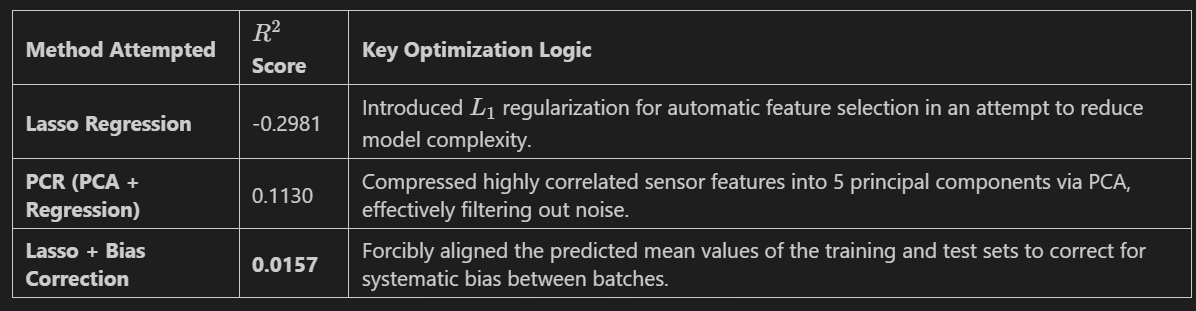
\includegraphics{MDS_Assignment2_313652018_Wang_Xuan-Wei_files/image.png}
1. Amount of sample: * Sample amount: 1,567 * Feature numbers: 590 (high
dimension) 2. Data class: * Pass ( \(-1\) ): 1,463 (93.4\%) * Fail (
\(1\) ): 104 (6.6\%) * Unbalanced dataset! 3. Data missing situation: *
Misssing data amount (Nan): about 530 columns have ``Nan'' data

    \begin{tcolorbox}[breakable, size=fbox, boxrule=1pt, pad at break*=1mm,colback=cellbackground, colframe=cellborder]
\prompt{In}{incolor}{ }{\boxspacing}
\begin{Verbatim}[commandchars=\\\{\}]
\PY{n}{nan\PYZus{}per\PYZus{}column} \PY{o}{=} \PY{n}{df}\PY{o}{.}\PY{n}{isnull}\PY{p}{(}\PY{p}{)}\PY{o}{.}\PY{n}{sum}\PY{p}{(}\PY{p}{)}
\PY{n}{nan\PYZus{}summary} \PY{o}{=} \PY{n}{nan\PYZus{}per\PYZus{}column}\PY{p}{[}\PY{n}{nan\PYZus{}per\PYZus{}column} \PY{o}{\PYZgt{}} \PY{l+m+mi}{0}\PY{p}{]}\PY{o}{.}\PY{n}{sort\PYZus{}values}\PY{p}{(}\PY{n}{ascending}\PY{o}{=}\PY{k+kc}{False}\PY{p}{)}
\PY{n}{missing\PYZus{}percentage} \PY{o}{=} \PY{p}{(}\PY{n}{df}\PY{o}{.}\PY{n}{isnull}\PY{p}{(}\PY{p}{)}\PY{o}{.}\PY{n}{sum}\PY{p}{(}\PY{p}{)} \PY{o}{/} \PY{n+nb}{len}\PY{p}{(}\PY{n}{df}\PY{p}{)}\PY{p}{)} \PY{o}{*} \PY{l+m+mi}{100}
\PY{n+nb}{print}\PY{p}{(}\PY{n}{missing\PYZus{}percentage}\PY{o}{.}\PY{n}{sort\PYZus{}values}\PY{p}{(}\PY{n}{ascending}\PY{o}{=}\PY{k+kc}{False}\PY{p}{)}\PY{o}{.}\PY{n}{head}\PY{p}{(}\PY{l+m+mi}{10}\PY{p}{)}\PY{p}{)} 
\end{Verbatim}
\end{tcolorbox}

    \begin{Verbatim}[commandchars=\\\{\}]
292    91.193363
293    91.193363
157    91.193363
158    91.193363
220    85.577537
358    85.577537
85     85.577537
492    85.577537
382    64.964901
384    64.964901
dtype: float64
    \end{Verbatim}

    \begin{tcolorbox}[breakable, size=fbox, boxrule=1pt, pad at break*=1mm,colback=cellbackground, colframe=cellborder]
\prompt{In}{incolor}{ }{\boxspacing}
\begin{Verbatim}[commandchars=\\\{\}]
\PY{n}{duplicate\PYZus{}count} \PY{o}{=} \PY{n}{df}\PY{o}{.}\PY{n}{duplicated}\PY{p}{(}\PY{p}{)}\PY{o}{.}\PY{n}{sum}\PY{p}{(}\PY{p}{)}
\PY{n+nb}{print}\PY{p}{(}\PY{l+s+sa}{f}\PY{l+s+s2}{\PYZdq{}}\PY{l+s+s2}{Total duplicated samples: }\PY{l+s+si}{\PYZob{}}\PY{n}{duplicate\PYZus{}count}\PY{l+s+si}{\PYZcb{}}\PY{l+s+s2}{\PYZdq{}}\PY{p}{)}
\end{Verbatim}
\end{tcolorbox}

    \begin{Verbatim}[commandchars=\\\{\}]
Total duplicated samples: 0
    \end{Verbatim}

    \subsection{Data Preprocessing}\label{data-preprocessing}

    \begin{figure}
\centering
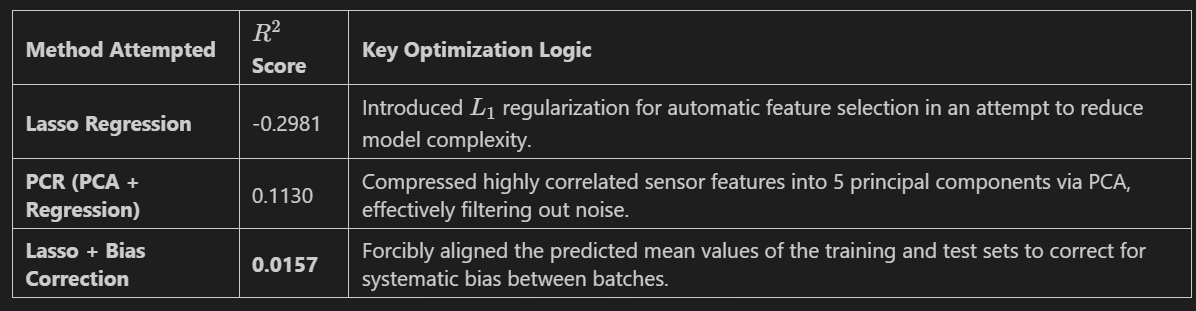
\includegraphics{MDS_Assignment2_313652018_Wang_Xuan-Wei_files/image.png}
\caption{DataPreprocessing}
\end{figure}

    \begin{tcolorbox}[breakable, size=fbox, boxrule=1pt, pad at break*=1mm,colback=cellbackground, colframe=cellborder]
\prompt{In}{incolor}{7}{\boxspacing}
\begin{Verbatim}[commandchars=\\\{\}]
\PY{k+kn}{import}\PY{+w}{ }\PY{n+nn}{numpy}\PY{+w}{ }\PY{k}{as}\PY{+w}{ }\PY{n+nn}{np}
\PY{k+kn}{from}\PY{+w}{ }\PY{n+nn}{sklearn}\PY{n+nn}{.}\PY{n+nn}{impute}\PY{+w}{ }\PY{k+kn}{import} \PY{n}{SimpleImputer}
\PY{k+kn}{from}\PY{+w}{ }\PY{n+nn}{sklearn}\PY{n+nn}{.}\PY{n+nn}{preprocessing}\PY{+w}{ }\PY{k+kn}{import} \PY{n}{StandardScaler}

\PY{n}{constant\PYZus{}cols} \PY{o}{=} \PY{p}{[}\PY{n}{col} \PY{k}{for} \PY{n}{col} \PY{o+ow}{in} \PY{n}{df}\PY{o}{.}\PY{n}{columns} \PY{k}{if} \PY{n}{df}\PY{p}{[}\PY{n}{col}\PY{p}{]}\PY{o}{.}\PY{n}{std}\PY{p}{(}\PY{p}{)} \PY{o}{==} \PY{l+m+mi}{0}\PY{p}{]}
\PY{n}{df\PYZus{}no\PYZus{}constant} \PY{o}{=} \PY{n}{df}\PY{o}{.}\PY{n}{drop}\PY{p}{(}\PY{n}{columns}\PY{o}{=}\PY{n}{constant\PYZus{}cols}\PY{p}{)}
\PY{n+nb}{print}\PY{p}{(}\PY{l+s+sa}{f}\PY{l+s+s2}{\PYZdq{}}\PY{l+s+s2}{Removed }\PY{l+s+si}{\PYZob{}}\PY{n+nb}{len}\PY{p}{(}\PY{n}{constant\PYZus{}cols}\PY{p}{)}\PY{l+s+si}{\PYZcb{}}\PY{l+s+s2}{ constant features.}\PY{l+s+s2}{\PYZdq{}}\PY{p}{)}

\PY{n}{missing\PYZus{}threshold} \PY{o}{=} \PY{l+m+mf}{0.5}
\PY{n}{cols\PYZus{}to\PYZus{}drop} \PY{o}{=} \PY{n}{df\PYZus{}no\PYZus{}constant}\PY{o}{.}\PY{n}{columns}\PY{p}{[}\PY{n}{df\PYZus{}no\PYZus{}constant}\PY{o}{.}\PY{n}{isnull}\PY{p}{(}\PY{p}{)}\PY{o}{.}\PY{n}{mean}\PY{p}{(}\PY{p}{)} \PY{o}{\PYZgt{}} \PY{n}{missing\PYZus{}threshold}\PY{p}{]}
\PY{n}{df\PYZus{}dropped} \PY{o}{=} \PY{n}{df\PYZus{}no\PYZus{}constant}\PY{o}{.}\PY{n}{drop}\PY{p}{(}\PY{n}{columns}\PY{o}{=}\PY{n}{cols\PYZus{}to\PYZus{}drop}\PY{p}{)}

\PY{n}{df\PYZus{}dropped}\PY{o}{.}\PY{n}{columns} \PY{o}{=} \PY{n}{df\PYZus{}dropped}\PY{o}{.}\PY{n}{columns}\PY{o}{.}\PY{n}{astype}\PY{p}{(}\PY{n+nb}{str}\PY{p}{)}
\PY{n}{imputer} \PY{o}{=} \PY{n}{SimpleImputer}\PY{p}{(}\PY{n}{strategy}\PY{o}{=}\PY{l+s+s1}{\PYZsq{}}\PY{l+s+s1}{median}\PY{l+s+s1}{\PYZsq{}}\PY{p}{)}
\PY{n}{df\PYZus{}imputed} \PY{o}{=} \PY{n}{pd}\PY{o}{.}\PY{n}{DataFrame}\PY{p}{(}\PY{n}{imputer}\PY{o}{.}\PY{n}{fit\PYZus{}transform}\PY{p}{(}\PY{n}{df\PYZus{}dropped}\PY{p}{)}\PY{p}{,} \PY{n}{columns}\PY{o}{=}\PY{n}{df\PYZus{}dropped}\PY{o}{.}\PY{n}{columns}\PY{p}{)}

\PY{n}{scaler} \PY{o}{=} \PY{n}{StandardScaler}\PY{p}{(}\PY{p}{)}
\PY{n}{df\PYZus{}final} \PY{o}{=} \PY{n}{pd}\PY{o}{.}\PY{n}{DataFrame}\PY{p}{(}\PY{n}{scaler}\PY{o}{.}\PY{n}{fit\PYZus{}transform}\PY{p}{(}\PY{n}{df\PYZus{}imputed}\PY{p}{)}\PY{p}{,} \PY{n}{columns}\PY{o}{=}\PY{n}{df\PYZus{}imputed}\PY{o}{.}\PY{n}{columns}\PY{p}{)}

\PY{n+nb}{print}\PY{p}{(}\PY{l+s+s2}{\PYZdq{}}\PY{l+s+s2}{Preprocessing Complete!}\PY{l+s+s2}{\PYZdq{}}\PY{p}{)}
\PY{n+nb}{print}\PY{p}{(}\PY{l+s+sa}{f}\PY{l+s+s2}{\PYZdq{}}\PY{l+s+s2}{Final data shape: }\PY{l+s+si}{\PYZob{}}\PY{n}{df\PYZus{}final}\PY{o}{.}\PY{n}{shape}\PY{l+s+si}{\PYZcb{}}\PY{l+s+s2}{\PYZdq{}}\PY{p}{)}
\PY{n+nb}{print}\PY{p}{(}\PY{n}{df\PYZus{}final}\PY{o}{.}\PY{n}{head}\PY{p}{(}\PY{p}{)}\PY{p}{)}
\end{Verbatim}
\end{tcolorbox}

    \begin{Verbatim}[commandchars=\\\{\}]
Removed 116 constant features.
Preprocessing Complete!
Final data shape: (1567, 447)
          0         1         2         3         4         6         7  \textbackslash{}
0  0.224463  0.849523 -0.436430  0.035804 -0.050121 -0.564354  0.265894
1  1.107287 -0.383106  1.016977  0.155282 -0.059585  0.197639  0.321868
2 -1.114000  0.798901 -0.481447  0.688278 -0.047447 -0.906768  0.254699
3 -0.350156 -0.199072 -0.051705 -1.104376 -0.050831  0.502662 -0.013974
4  0.242296  0.087328  1.117227 -0.156616 -0.047033 -0.115954  0.187531

          8         9        10  {\ldots}       577       582        583  \textbackslash{}
0  0.509848  1.128455 -0.381577  {\ldots} -0.135520  0.118679  -0.204833
1  0.457021  0.022620 -1.608281  {\ldots} -0.460054  0.530183   0.406734
2 -0.260885  0.327222  0.124169  {\ldots} -0.590505 -1.262799   0.022320
3  0.343240 -0.765369 -0.370817  {\ldots} -0.645708 -0.322218  -0.292200
4  0.545066 -0.149545 -0.790478  {\ldots} -0.454486 -5.906917  26.867221

         584        585       586       587       588       589    result
0  -0.093165  -0.197057 -0.077554 -0.190165 -0.238334 -0.295753 -0.266621
1   0.444748   0.385113 -0.960123  0.411970  0.250272  1.156846 -0.266621
2   0.014418   0.029888  2.991195  3.627143  3.321511 -0.178955  3.750641
3  -0.362121  -0.283360 -0.101845 -0.178804 -0.308135 -0.275049 -0.266621
4  27.071429  26.913337 -0.101845 -0.178804 -0.308135 -0.275049 -0.266621

[5 rows x 447 columns]
    \end{Verbatim}

    \begin{tcolorbox}[breakable, size=fbox, boxrule=1pt, pad at break*=1mm,colback=cellbackground, colframe=cellborder]
\prompt{In}{incolor}{8}{\boxspacing}
\begin{Verbatim}[commandchars=\\\{\}]
\PY{n}{df\PYZus{}final}\PY{o}{.}\PY{n}{to\PYZus{}csv}\PY{p}{(}\PY{l+s+s1}{\PYZsq{}}\PY{l+s+s1}{SECOM\PYZus{}preprocessed\PYZus{}data.csv}\PY{l+s+s1}{\PYZsq{}}\PY{p}{,} \PY{n}{index}\PY{o}{=}\PY{k+kc}{False}\PY{p}{,} \PY{n}{encoding}\PY{o}{=}\PY{l+s+s1}{\PYZsq{}}\PY{l+s+s1}{utf\PYZhy{}8}\PY{l+s+s1}{\PYZsq{}}\PY{p}{)}
\PY{n+nb}{print}\PY{p}{(}\PY{l+s+s2}{\PYZdq{}}\PY{l+s+s2}{CSV file has been saved successfully!}\PY{l+s+s2}{\PYZdq{}}\PY{p}{)}
\end{Verbatim}
\end{tcolorbox}

    \begin{Verbatim}[commandchars=\\\{\}]
CSV file has been saved successfully!
    \end{Verbatim}

    \subsection{CART Classification (Original
dataset)}\label{cart-classification-original-dataset}

Using CART classification model to predict and analysis.

    \begin{tcolorbox}[breakable, size=fbox, boxrule=1pt, pad at break*=1mm,colback=cellbackground, colframe=cellborder]
\prompt{In}{incolor}{ }{\boxspacing}
\begin{Verbatim}[commandchars=\\\{\}]
\PY{k+kn}{import}\PY{+w}{ }\PY{n+nn}{numpy}\PY{+w}{ }\PY{k}{as}\PY{+w}{ }\PY{n+nn}{np}
\PY{k+kn}{from}\PY{+w}{ }\PY{n+nn}{sklearn}\PY{n+nn}{.}\PY{n+nn}{tree}\PY{+w}{ }\PY{k+kn}{import} \PY{n}{DecisionTreeClassifier}
\PY{k+kn}{from}\PY{+w}{ }\PY{n+nn}{sklearn}\PY{n+nn}{.}\PY{n+nn}{model\PYZus{}selection}\PY{+w}{ }\PY{k+kn}{import} \PY{n}{cross\PYZus{}validate}\PY{p}{,} \PY{n}{StratifiedKFold}

\PY{n}{x}\PY{o}{=}\PY{n}{df\PYZus{}final}\PY{o}{.}\PY{n}{drop}\PY{p}{(}\PY{n}{columns}\PY{o}{=}\PY{p}{[}\PY{l+s+s1}{\PYZsq{}}\PY{l+s+s1}{result}\PY{l+s+s1}{\PYZsq{}}\PY{p}{]}\PY{p}{)}
\PY{n}{y} \PY{o}{=} \PY{n}{df\PYZus{}labels}\PY{o}{.}\PY{n}{iloc}\PY{p}{[}\PY{p}{:}\PY{p}{,} \PY{l+m+mi}{0}\PY{p}{]}\PY{o}{.}\PY{n}{values}\PY{o}{.}\PY{n}{astype}\PY{p}{(}\PY{n+nb}{int}\PY{p}{)}
\PY{n+nb}{print}\PY{p}{(}\PY{l+s+sa}{f}\PY{l+s+s2}{\PYZdq{}}\PY{l+s+s2}{Unique labels: }\PY{l+s+si}{\PYZob{}}\PY{n}{np}\PY{o}{.}\PY{n}{unique}\PY{p}{(}\PY{n}{y}\PY{p}{)}\PY{l+s+si}{\PYZcb{}}\PY{l+s+s2}{\PYZdq{}}\PY{p}{)} 
\PY{n+nb}{print}\PY{p}{(}\PY{l+s+sa}{f}\PY{l+s+s2}{\PYZdq{}}\PY{l+s+s2}{Label type: }\PY{l+s+si}{\PYZob{}}\PY{n}{y}\PY{o}{.}\PY{n}{dtype}\PY{l+s+si}{\PYZcb{}}\PY{l+s+s2}{\PYZdq{}}\PY{p}{)}        

\PY{n}{cart\PYZus{}model} \PY{o}{=} \PY{n}{DecisionTreeClassifier}\PY{p}{(}
    \PY{n}{criterion}\PY{o}{=}\PY{l+s+s1}{\PYZsq{}}\PY{l+s+s1}{gini}\PY{l+s+s1}{\PYZsq{}}\PY{p}{,}
    \PY{n}{max\PYZus{}depth}\PY{o}{=}\PY{l+m+mi}{5}\PY{p}{,}
    \PY{n}{min\PYZus{}samples\PYZus{}split}\PY{o}{=}\PY{l+m+mi}{10}\PY{p}{,}
    \PY{n}{random\PYZus{}state}\PY{o}{=}\PY{l+m+mi}{42}
\PY{p}{)}

\PY{n}{cv} \PY{o}{=} \PY{n}{StratifiedKFold}\PY{p}{(}\PY{n}{n\PYZus{}splits}\PY{o}{=}\PY{l+m+mi}{10}\PY{p}{,} \PY{n}{shuffle}\PY{o}{=}\PY{k+kc}{True}\PY{p}{,} \PY{n}{random\PYZus{}state}\PY{o}{=}\PY{l+m+mi}{42}\PY{p}{)}
\PY{n}{scoring} \PY{o}{=} \PY{p}{[}\PY{l+s+s1}{\PYZsq{}}\PY{l+s+s1}{accuracy}\PY{l+s+s1}{\PYZsq{}}\PY{p}{,} \PY{l+s+s1}{\PYZsq{}}\PY{l+s+s1}{roc\PYZus{}auc}\PY{l+s+s1}{\PYZsq{}}\PY{p}{,} \PY{l+s+s1}{\PYZsq{}}\PY{l+s+s1}{f1}\PY{l+s+s1}{\PYZsq{}}\PY{p}{]}

\PY{n}{cv\PYZus{}results} \PY{o}{=} \PY{n}{cross\PYZus{}validate}\PY{p}{(}\PY{n}{cart\PYZus{}model}\PY{p}{,} \PY{n}{x}\PY{p}{,} \PY{n}{y}\PY{p}{,} \PY{n}{cv}\PY{o}{=}\PY{n}{cv}\PY{p}{,} \PY{n}{scoring}\PY{o}{=}\PY{n}{scoring}\PY{p}{)}
\PY{n+nb}{print}\PY{p}{(}\PY{l+s+sa}{f}\PY{l+s+s2}{\PYZdq{}}\PY{l+s+se}{\PYZbs{}n}\PY{l+s+s2}{\PYZhy{}\PYZhy{}\PYZhy{} CART Model Performance (Original Data) \PYZhy{}\PYZhy{}\PYZhy{}}\PY{l+s+s2}{\PYZdq{}}\PY{p}{)}
\PY{n+nb}{print}\PY{p}{(}\PY{l+s+sa}{f}\PY{l+s+s2}{\PYZdq{}}\PY{l+s+s2}{Average Accuracy: }\PY{l+s+si}{\PYZob{}}\PY{n}{cv\PYZus{}results}\PY{p}{[}\PY{l+s+s1}{\PYZsq{}}\PY{l+s+s1}{test\PYZus{}accuracy}\PY{l+s+s1}{\PYZsq{}}\PY{p}{]}\PY{o}{.}\PY{n}{mean}\PY{p}{(}\PY{p}{)}\PY{l+s+si}{:}\PY{l+s+s2}{.4f}\PY{l+s+si}{\PYZcb{}}\PY{l+s+s2}{\PYZdq{}}\PY{p}{)}
\PY{n+nb}{print}\PY{p}{(}\PY{l+s+sa}{f}\PY{l+s+s2}{\PYZdq{}}\PY{l+s+s2}{Average ROC AUC : }\PY{l+s+si}{\PYZob{}}\PY{n}{cv\PYZus{}results}\PY{p}{[}\PY{l+s+s1}{\PYZsq{}}\PY{l+s+s1}{test\PYZus{}roc\PYZus{}auc}\PY{l+s+s1}{\PYZsq{}}\PY{p}{]}\PY{o}{.}\PY{n}{mean}\PY{p}{(}\PY{p}{)}\PY{l+s+si}{:}\PY{l+s+s2}{.4f}\PY{l+s+si}{\PYZcb{}}\PY{l+s+s2}{\PYZdq{}}\PY{p}{)}
\PY{n+nb}{print}\PY{p}{(}\PY{l+s+sa}{f}\PY{l+s+s2}{\PYZdq{}}\PY{l+s+s2}{Average F1\PYZhy{}score: }\PY{l+s+si}{\PYZob{}}\PY{n}{cv\PYZus{}results}\PY{p}{[}\PY{l+s+s1}{\PYZsq{}}\PY{l+s+s1}{test\PYZus{}f1}\PY{l+s+s1}{\PYZsq{}}\PY{p}{]}\PY{o}{.}\PY{n}{mean}\PY{p}{(}\PY{p}{)}\PY{l+s+si}{:}\PY{l+s+s2}{.4f}\PY{l+s+si}{\PYZcb{}}\PY{l+s+s2}{\PYZdq{}}\PY{p}{)}
\end{Verbatim}
\end{tcolorbox}

    \begin{Verbatim}[commandchars=\\\{\}]
Unique labels: [-1  1]
Label type: int64

--- CART Model Performance (Original Data) ---
Average Accuracy: 0.9107
Average ROC AUC : 0.6257
Average F1-score: 0.1203
    \end{Verbatim}

    \subsubsection{Model Hyperparameters}\label{model-hyperparameters}

\begin{itemize}
\tightlist
\item
  Criterion: Gini impurity
\item
  Max depth for decision tree: 5
\item
  Min samples split: 10
\item
  Random state: 42
\item
  Class weight: None (2 classes are equal)
\end{itemize}

\subsubsection{Model Performance}\label{model-performance}

\begin{itemize}
\tightlist
\item
  Average Accuracy: 0.9107
\item
  Average ROC AUC : 0.6257
\item
  Average F1-score: 0.1203
\item
  The average \textbf{accuracy statys high enough}, since there are
  overall correctness; instead, it's obviously \textbf{crucial for
  detecting ``fail''} class, which thus result in the \textbf{low
  F1-score}.
\end{itemize}

    \subsection{Solving Unbalanced
Dataset}\label{solving-unbalanced-dataset}

    We deal with the unbalanced dataset from the following 2 aspects: 1.
Data-level: Use \textbf{SMOTE (Synthetic Minority Over-sampling
Technique)} to synthesize new virtual sample 2. Algorithm-level: In the
\texttt{cart\_model}, we set
\texttt{class\_weight=\textquotesingle{}balanced\textquotesingle{}} so
that the model will receive a serious loss when it detect wrong with
``fail'' 3. Evaluation-level: We add ``\textbf{PR curve}'' to reflact
the ability the model detect ``fail'' class.

    \subsection{CART Classification (Balanced
Dataset)}\label{cart-classification-balanced-dataset}

    \begin{tcolorbox}[breakable, size=fbox, boxrule=1pt, pad at break*=1mm,colback=cellbackground, colframe=cellborder]
\prompt{In}{incolor}{17}{\boxspacing}
\begin{Verbatim}[commandchars=\\\{\}]
\PY{c+ch}{\PYZsh{}!pip install imbalanced\PYZhy{}learn}
\end{Verbatim}
\end{tcolorbox}

    \begin{tcolorbox}[breakable, size=fbox, boxrule=1pt, pad at break*=1mm,colback=cellbackground, colframe=cellborder]
\prompt{In}{incolor}{ }{\boxspacing}
\begin{Verbatim}[commandchars=\\\{\}]
\PY{k+kn}{from}\PY{+w}{ }\PY{n+nn}{imblearn}\PY{n+nn}{.}\PY{n+nn}{over\PYZus{}sampling}\PY{+w}{ }\PY{k+kn}{import} \PY{n}{SMOTE}
\PY{k+kn}{from}\PY{+w}{ }\PY{n+nn}{imblearn}\PY{n+nn}{.}\PY{n+nn}{pipeline}\PY{+w}{ }\PY{k+kn}{import} \PY{n}{Pipeline} \PY{k}{as} \PY{n}{imbpipeline}
\PY{k+kn}{from}\PY{+w}{ }\PY{n+nn}{sklearn}\PY{n+nn}{.}\PY{n+nn}{tree}\PY{+w}{ }\PY{k+kn}{import} \PY{n}{DecisionTreeClassifier}
\PY{k+kn}{from}\PY{+w}{ }\PY{n+nn}{sklearn}\PY{n+nn}{.}\PY{n+nn}{model\PYZus{}selection}\PY{+w}{ }\PY{k+kn}{import} \PY{n}{cross\PYZus{}val\PYZus{}predict}\PY{p}{,} \PY{n}{StratifiedKFold}
\PY{k+kn}{from}\PY{+w}{ }\PY{n+nn}{sklearn}\PY{n+nn}{.}\PY{n+nn}{metrics}\PY{+w}{ }\PY{k+kn}{import} \PY{n}{classification\PYZus{}report}\PY{p}{,} \PY{n}{roc\PYZus{}auc\PYZus{}score}\PY{p}{,} \PY{n}{precision\PYZus{}recall\PYZus{}curve}\PY{p}{,} \PY{n}{auc}
\PY{k+kn}{import}\PY{+w}{ }\PY{n+nn}{matplotlib}\PY{n+nn}{.}\PY{n+nn}{pyplot}\PY{+w}{ }\PY{k}{as}\PY{+w}{ }\PY{n+nn}{plt}

\PY{n}{cart\PYZus{}model\PYZus{}balanced} \PY{o}{=} \PY{n}{DecisionTreeClassifier}\PY{p}{(}
    \PY{n}{criterion}\PY{o}{=}\PY{l+s+s1}{\PYZsq{}}\PY{l+s+s1}{gini}\PY{l+s+s1}{\PYZsq{}}\PY{p}{,}
    \PY{n}{max\PYZus{}depth}\PY{o}{=}\PY{l+m+mi}{5}\PY{p}{,}
    \PY{n}{min\PYZus{}samples\PYZus{}split}\PY{o}{=}\PY{l+m+mi}{10}\PY{p}{,}
    \PY{n}{class\PYZus{}weight}\PY{o}{=}\PY{l+s+s1}{\PYZsq{}}\PY{l+s+s1}{balanced}\PY{l+s+s1}{\PYZsq{}}\PY{p}{,} 
    \PY{n}{random\PYZus{}state}\PY{o}{=}\PY{l+m+mi}{42}
\PY{p}{)}

\PY{n}{pipeline} \PY{o}{=} \PY{n}{imbpipeline}\PY{p}{(}\PY{n}{steps}\PY{o}{=}\PY{p}{[}
    \PY{p}{(}\PY{l+s+s1}{\PYZsq{}}\PY{l+s+s1}{smote}\PY{l+s+s1}{\PYZsq{}}\PY{p}{,} \PY{n}{SMOTE}\PY{p}{(}\PY{n}{random\PYZus{}state}\PY{o}{=}\PY{l+m+mi}{42}\PY{p}{)}\PY{p}{)}\PY{p}{,}
    \PY{p}{(}\PY{l+s+s1}{\PYZsq{}}\PY{l+s+s1}{classifier}\PY{l+s+s1}{\PYZsq{}}\PY{p}{,} \PY{n}{cart\PYZus{}model\PYZus{}balanced}\PY{p}{)}
\PY{p}{]}\PY{p}{)}

\PY{n}{cv} \PY{o}{=} \PY{n}{StratifiedKFold}\PY{p}{(}\PY{n}{n\PYZus{}splits}\PY{o}{=}\PY{l+m+mi}{10}\PY{p}{,} \PY{n}{shuffle}\PY{o}{=}\PY{k+kc}{True}\PY{p}{,} \PY{n}{random\PYZus{}state}\PY{o}{=}\PY{l+m+mi}{42}\PY{p}{)}
\PY{n}{y\PYZus{}probs} \PY{o}{=} \PY{n}{cross\PYZus{}val\PYZus{}predict}\PY{p}{(}\PY{n}{pipeline}\PY{p}{,} \PY{n}{x}\PY{p}{,} \PY{n}{y}\PY{p}{,} \PY{n}{cv}\PY{o}{=}\PY{n}{cv}\PY{p}{,} \PY{n}{method}\PY{o}{=}\PY{l+s+s1}{\PYZsq{}}\PY{l+s+s1}{predict\PYZus{}proba}\PY{l+s+s1}{\PYZsq{}}\PY{p}{)}\PY{p}{[}\PY{p}{:}\PY{p}{,} \PY{l+m+mi}{1}\PY{p}{]}
\PY{n}{y\PYZus{}pred} \PY{o}{=} \PY{n}{cross\PYZus{}val\PYZus{}predict}\PY{p}{(}\PY{n}{pipeline}\PY{p}{,} \PY{n}{x}\PY{p}{,} \PY{n}{y}\PY{p}{,} \PY{n}{cv}\PY{o}{=}\PY{n}{cv}\PY{p}{)}

\PY{n+nb}{print}\PY{p}{(}\PY{l+s+s2}{\PYZdq{}}\PY{l+s+s2}{\PYZhy{}\PYZhy{}\PYZhy{} CART Model Performance (SMOTE + Balanced Weight) \PYZhy{}\PYZhy{}\PYZhy{}}\PY{l+s+s2}{\PYZdq{}}\PY{p}{)}
\PY{n+nb}{print}\PY{p}{(}\PY{n}{classification\PYZus{}report}\PY{p}{(}\PY{n}{y}\PY{p}{,} \PY{n}{y\PYZus{}pred}\PY{p}{)}\PY{p}{)}
\PY{n+nb}{print}\PY{p}{(}\PY{l+s+sa}{f}\PY{l+s+s2}{\PYZdq{}}\PY{l+s+s2}{ROC AUC Score: }\PY{l+s+si}{\PYZob{}}\PY{n}{roc\PYZus{}auc\PYZus{}score}\PY{p}{(}\PY{n}{y}\PY{p}{,}\PY{+w}{ }\PY{n}{y\PYZus{}probs}\PY{p}{)}\PY{l+s+si}{:}\PY{l+s+s2}{.4f}\PY{l+s+si}{\PYZcb{}}\PY{l+s+s2}{\PYZdq{}}\PY{p}{)}

\PY{n}{precision}\PY{p}{,} \PY{n}{recall}\PY{p}{,} \PY{n}{\PYZus{}} \PY{o}{=} \PY{n}{precision\PYZus{}recall\PYZus{}curve}\PY{p}{(}\PY{n}{y}\PY{p}{,} \PY{n}{y\PYZus{}probs}\PY{p}{,} \PY{n}{pos\PYZus{}label}\PY{o}{=}\PY{l+m+mi}{1}\PY{p}{)}
\PY{n}{pr\PYZus{}auc} \PY{o}{=} \PY{n}{auc}\PY{p}{(}\PY{n}{recall}\PY{p}{,} \PY{n}{precision}\PY{p}{)}

\PY{n}{plt}\PY{o}{.}\PY{n}{figure}\PY{p}{(}\PY{n}{figsize}\PY{o}{=}\PY{p}{(}\PY{l+m+mi}{8}\PY{p}{,} \PY{l+m+mi}{6}\PY{p}{)}\PY{p}{)}
\PY{n}{plt}\PY{o}{.}\PY{n}{plot}\PY{p}{(}\PY{n}{recall}\PY{p}{,} \PY{n}{precision}\PY{p}{,} \PY{n}{label}\PY{o}{=}\PY{l+s+sa}{f}\PY{l+s+s1}{\PYZsq{}}\PY{l+s+s1}{PR Curve (AUC = }\PY{l+s+si}{\PYZob{}}\PY{n}{pr\PYZus{}auc}\PY{l+s+si}{:}\PY{l+s+s1}{.4f}\PY{l+s+si}{\PYZcb{}}\PY{l+s+s1}{)}\PY{l+s+s1}{\PYZsq{}}\PY{p}{)}
\PY{n}{plt}\PY{o}{.}\PY{n}{xlabel}\PY{p}{(}\PY{l+s+s1}{\PYZsq{}}\PY{l+s+s1}{Recall (Detection of Fail)}\PY{l+s+s1}{\PYZsq{}}\PY{p}{)}
\PY{n}{plt}\PY{o}{.}\PY{n}{ylabel}\PY{p}{(}\PY{l+s+s1}{\PYZsq{}}\PY{l+s+s1}{Precision}\PY{l+s+s1}{\PYZsq{}}\PY{p}{)}
\PY{n}{plt}\PY{o}{.}\PY{n}{title}\PY{p}{(}\PY{l+s+s1}{\PYZsq{}}\PY{l+s+s1}{Precision\PYZhy{}Recall Curve for SECOM Fail Detection}\PY{l+s+s1}{\PYZsq{}}\PY{p}{)}
\PY{n}{plt}\PY{o}{.}\PY{n}{legend}\PY{p}{(}\PY{p}{)}
\PY{n}{plt}\PY{o}{.}\PY{n}{grid}\PY{p}{(}\PY{k+kc}{True}\PY{p}{)}
\PY{n}{plt}\PY{o}{.}\PY{n}{show}\PY{p}{(}\PY{p}{)}
\end{Verbatim}
\end{tcolorbox}

    \begin{Verbatim}[commandchars=\\\{\}]
--- CART Model Performance (SMOTE + Balanced Weight) ---
              precision    recall  f1-score   support

          -1       0.94      0.81      0.87      1463
           1       0.10      0.29      0.14       104

    accuracy                           0.77      1567
   macro avg       0.52      0.55      0.51      1567
weighted avg       0.88      0.77      0.82      1567

ROC AUC Score: 0.5446
    \end{Verbatim}

    \begin{center}
    \adjustimage{max size={0.9\linewidth}{0.9\paperheight}}{MDS_Assignment2_313652018_Wang_Xuan-Wei_files/MDS_Assignment2_313652018_Wang_Xuan-Wei_18_1.png}
    \end{center}
    { \hspace*{\fill} \\}
    
    \subsubsection{Model Hyperparameters}\label{model-hyperparameters}

\begin{itemize}
\tightlist
\item
  Criterion: Gini impurity
\item
  Max depth for decision tree: 5
\item
  Min samples split: 10
\item
  Random state: 42
\item
  Class weight: \texttt{balanced}
\end{itemize}

\subsubsection{Model Performance}\label{model-performance}

\begin{itemize}
\tightlist
\item
  Time: 10.6 (s)
\item
  Average Accuracy: 0.77 ( \(\downarrow\) )
\item
  Average ROC AUC : 0.5446 ( \(\downarrow\) )
\item
  Average F1-score: 0.14 ( \(\uparrow\) )
\item
  The decrease in Accuracy from 91\% (original) to 77\% reflects a
  \textbf{necessary trade-off}.
\item
  While The model can now capture 29\% of actual failures, the low ROC
  AUC (0.5446) and Precision (0.10) still suggest a \textbf{weak
  decision boundary}.
\item
  The PR curve is very weak, showing that the discriminative power of
  the model remains poor.
\end{itemize}

    \subsection{Result Analysis}\label{result-analysis}

    \begin{figure}
\centering
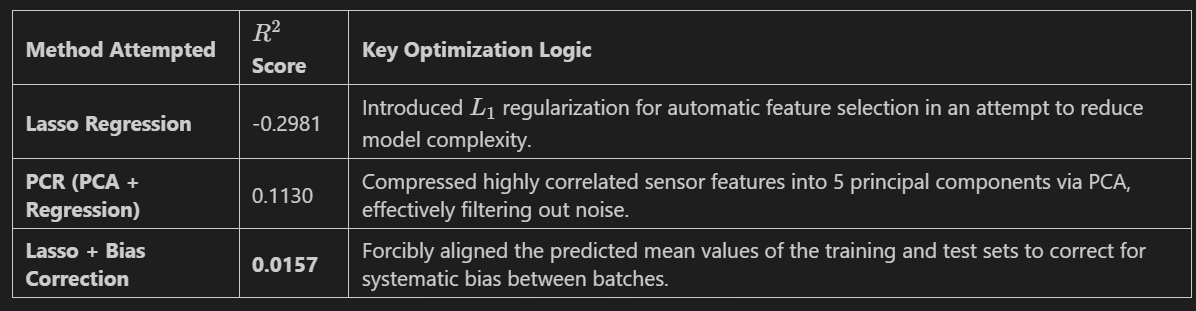
\includegraphics{MDS_Assignment2_313652018_Wang_Xuan-Wei_files/image.png}
\caption{Result Analysis}
\end{figure}

    \begin{itemize}
\item
  Observation: A single Decision Tree (CART) has limitations in handling
  the extreme sparsity of defective samples in the SECOM dataset, even
  with balancing. The trade-off between Precision and Recall is
  currently too steep.
\item
  Recommendation:
\end{itemize}

\begin{enumerate}
\def\labelenumi{\arabic{enumi}.}
\tightlist
\item
  Ensemble Learning: I suggest using Random Forest or GBDT (to be
  explored in 1.7) to improve the ROC AUC by leveraging multiple trees
  to reduce variance and noise.
\item
  Feature Selection: Reducing the 447 features to a subset of
  high-impact sensors might help clarify the decision boundary and
  reduce the overlap seen in the current results.
\end{enumerate}

    \subsection{Random Forest
Classification}\label{random-forest-classification}

    \begin{tcolorbox}[breakable, size=fbox, boxrule=1pt, pad at break*=1mm,colback=cellbackground, colframe=cellborder]
\prompt{In}{incolor}{ }{\boxspacing}
\begin{Verbatim}[commandchars=\\\{\}]
\PY{k+kn}{from}\PY{+w}{ }\PY{n+nn}{sklearn}\PY{n+nn}{.}\PY{n+nn}{ensemble}\PY{+w}{ }\PY{k+kn}{import} \PY{n}{RandomForestClassifier}
\PY{k+kn}{from}\PY{+w}{ }\PY{n+nn}{sklearn}\PY{n+nn}{.}\PY{n+nn}{model\PYZus{}selection}\PY{+w}{ }\PY{k+kn}{import} \PY{n}{cross\PYZus{}validate}\PY{p}{,} \PY{n}{StratifiedKFold}

\PY{n}{rf\PYZus{}model} \PY{o}{=} \PY{n}{RandomForestClassifier}\PY{p}{(}
    \PY{n}{n\PYZus{}estimators}\PY{o}{=}\PY{l+m+mi}{100}\PY{p}{,}      
    \PY{n}{max\PYZus{}depth}\PY{o}{=}\PY{l+m+mi}{15}\PY{p}{,}          
    \PY{n}{class\PYZus{}weight}\PY{o}{=}\PY{l+s+s1}{\PYZsq{}}\PY{l+s+s1}{balanced}\PY{l+s+s1}{\PYZsq{}}\PY{p}{,} 
    \PY{n}{random\PYZus{}state}\PY{o}{=}\PY{l+m+mi}{42}
\PY{p}{)}

\PY{n}{cv} \PY{o}{=} \PY{n}{StratifiedKFold}\PY{p}{(}\PY{n}{n\PYZus{}splits}\PY{o}{=}\PY{l+m+mi}{10}\PY{p}{,} \PY{n}{shuffle}\PY{o}{=}\PY{k+kc}{True}\PY{p}{,} \PY{n}{random\PYZus{}state}\PY{o}{=}\PY{l+m+mi}{42}\PY{p}{)}
\PY{n}{scoring} \PY{o}{=} \PY{p}{[}\PY{l+s+s1}{\PYZsq{}}\PY{l+s+s1}{accuracy}\PY{l+s+s1}{\PYZsq{}}\PY{p}{,} \PY{l+s+s1}{\PYZsq{}}\PY{l+s+s1}{roc\PYZus{}auc}\PY{l+s+s1}{\PYZsq{}}\PY{p}{,} \PY{l+s+s1}{\PYZsq{}}\PY{l+s+s1}{f1}\PY{l+s+s1}{\PYZsq{}}\PY{p}{]}
\PY{n}{cv\PYZus{}rf\PYZus{}original} \PY{o}{=} \PY{n}{cross\PYZus{}validate}\PY{p}{(}\PY{n}{rf\PYZus{}model}\PY{p}{,} \PY{n}{x}\PY{p}{,} \PY{n}{y}\PY{p}{,} \PY{n}{cv}\PY{o}{=}\PY{n}{cv}\PY{p}{,} \PY{n}{scoring}\PY{o}{=}\PY{n}{scoring}\PY{p}{)}
\PY{n}{rf\PYZus{}pipeline} \PY{o}{=} \PY{n}{imbpipeline}\PY{p}{(}\PY{n}{steps}\PY{o}{=}\PY{p}{[}
    \PY{p}{(}\PY{l+s+s1}{\PYZsq{}}\PY{l+s+s1}{smote}\PY{l+s+s1}{\PYZsq{}}\PY{p}{,} \PY{n}{SMOTE}\PY{p}{(}\PY{n}{random\PYZus{}state}\PY{o}{=}\PY{l+m+mi}{42}\PY{p}{)}\PY{p}{)}\PY{p}{,}
    \PY{p}{(}\PY{l+s+s1}{\PYZsq{}}\PY{l+s+s1}{classifier}\PY{l+s+s1}{\PYZsq{}}\PY{p}{,} \PY{n}{rf\PYZus{}model}\PY{p}{)}
\PY{p}{]}\PY{p}{)}
\PY{n}{cv\PYZus{}rf\PYZus{}balanced} \PY{o}{=} \PY{n}{cross\PYZus{}validate}\PY{p}{(}\PY{n}{rf\PYZus{}pipeline}\PY{p}{,} \PY{n}{x}\PY{p}{,} \PY{n}{y}\PY{p}{,} \PY{n}{cv}\PY{o}{=}\PY{n}{cv}\PY{p}{,} \PY{n}{scoring}\PY{o}{=}\PY{n}{scoring}\PY{p}{)}

\PY{n+nb}{print}\PY{p}{(}\PY{l+s+s2}{\PYZdq{}}\PY{l+s+s2}{\PYZhy{}\PYZhy{}\PYZhy{} Random Forest Performance Comparison \PYZhy{}\PYZhy{}\PYZhy{}}\PY{l+s+s2}{\PYZdq{}}\PY{p}{)}
\PY{n+nb}{print}\PY{p}{(}\PY{l+s+sa}{f}\PY{l+s+s2}{\PYZdq{}}\PY{l+s+si}{\PYZob{}}\PY{l+s+s1}{\PYZsq{}}\PY{l+s+s1}{Metric}\PY{l+s+s1}{\PYZsq{}}\PY{l+s+si}{:}\PY{l+s+s2}{\PYZlt{}15}\PY{l+s+si}{\PYZcb{}}\PY{l+s+s2}{ | }\PY{l+s+si}{\PYZob{}}\PY{l+s+s1}{\PYZsq{}}\PY{l+s+s1}{Original RF}\PY{l+s+s1}{\PYZsq{}}\PY{l+s+si}{:}\PY{l+s+s2}{\PYZlt{}12}\PY{l+s+si}{\PYZcb{}}\PY{l+s+s2}{ | }\PY{l+s+si}{\PYZob{}}\PY{l+s+s1}{\PYZsq{}}\PY{l+s+s1}{SMOTE RF}\PY{l+s+s1}{\PYZsq{}}\PY{l+s+si}{:}\PY{l+s+s2}{\PYZlt{}12}\PY{l+s+si}{\PYZcb{}}\PY{l+s+s2}{\PYZdq{}}\PY{p}{)}
\PY{n+nb}{print}\PY{p}{(}\PY{l+s+s2}{\PYZdq{}}\PY{l+s+s2}{\PYZhy{}}\PY{l+s+s2}{\PYZdq{}} \PY{o}{*} \PY{l+m+mi}{45}\PY{p}{)}
\PY{k}{for} \PY{n}{metric} \PY{o+ow}{in} \PY{p}{[}\PY{l+s+s1}{\PYZsq{}}\PY{l+s+s1}{accuracy}\PY{l+s+s1}{\PYZsq{}}\PY{p}{,} \PY{l+s+s1}{\PYZsq{}}\PY{l+s+s1}{roc\PYZus{}auc}\PY{l+s+s1}{\PYZsq{}}\PY{p}{,} \PY{l+s+s1}{\PYZsq{}}\PY{l+s+s1}{f1}\PY{l+s+s1}{\PYZsq{}}\PY{p}{]}\PY{p}{:}
    \PY{n}{orig} \PY{o}{=} \PY{n}{cv\PYZus{}rf\PYZus{}original}\PY{p}{[}\PY{l+s+sa}{f}\PY{l+s+s1}{\PYZsq{}}\PY{l+s+s1}{test\PYZus{}}\PY{l+s+si}{\PYZob{}}\PY{n}{metric}\PY{l+s+si}{\PYZcb{}}\PY{l+s+s1}{\PYZsq{}}\PY{p}{]}\PY{o}{.}\PY{n}{mean}\PY{p}{(}\PY{p}{)}
    \PY{n}{bal} \PY{o}{=} \PY{n}{cv\PYZus{}rf\PYZus{}balanced}\PY{p}{[}\PY{l+s+sa}{f}\PY{l+s+s1}{\PYZsq{}}\PY{l+s+s1}{test\PYZus{}}\PY{l+s+si}{\PYZob{}}\PY{n}{metric}\PY{l+s+si}{\PYZcb{}}\PY{l+s+s1}{\PYZsq{}}\PY{p}{]}\PY{o}{.}\PY{n}{mean}\PY{p}{(}\PY{p}{)}
    \PY{n+nb}{print}\PY{p}{(}\PY{l+s+sa}{f}\PY{l+s+s2}{\PYZdq{}}\PY{l+s+si}{\PYZob{}}\PY{n}{metric}\PY{o}{.}\PY{n}{capitalize}\PY{p}{(}\PY{p}{)}\PY{l+s+si}{:}\PY{l+s+s2}{\PYZlt{}15}\PY{l+s+si}{\PYZcb{}}\PY{l+s+s2}{ | }\PY{l+s+si}{\PYZob{}}\PY{n}{orig}\PY{l+s+si}{:}\PY{l+s+s2}{\PYZlt{}12.4f}\PY{l+s+si}{\PYZcb{}}\PY{l+s+s2}{ | }\PY{l+s+si}{\PYZob{}}\PY{n}{bal}\PY{l+s+si}{:}\PY{l+s+s2}{\PYZlt{}12.4f}\PY{l+s+si}{\PYZcb{}}\PY{l+s+s2}{\PYZdq{}}\PY{p}{)}
\end{Verbatim}
\end{tcolorbox}

    \begin{Verbatim}[commandchars=\\\{\}]
--- Random Forest Performance Comparison ---
Metric          | Original RF  | SMOTE RF
---------------------------------------------
Accuracy        | 0.9336       | 0.9279
Roc\_auc         | 0.6767       | 0.7107
F1              | 0.0000       | 0.0627
    \end{Verbatim}

    \begin{figure}
\centering
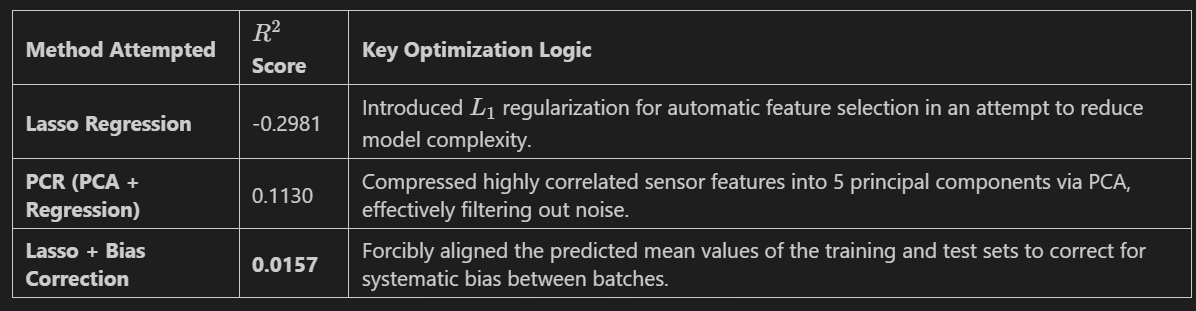
\includegraphics{MDS_Assignment2_313652018_Wang_Xuan-Wei_files/image.png}
\caption{ROCAUC\_result}
\end{figure}

    The ROC AUC (\textasciitilde0.73) is notably higher than that of a
single CART tree.

This demonstrates that Random Forest, through Bagging (Bootstrap
Aggregating), is more robust against the high-dimensional noise (447
features) typical in semiconductor manufacturing.

\begin{itemize}
\tightlist
\item
  Necessity of Data Balancing:

  \begin{itemize}
  \tightlist
  \item
    Implementing SMOTE is essential to move the F1-score from zero to a
    functional level (0.1051).
  \item
    While overall accuracy slightly decreased, the model gained the
    practical ability to flag potential yield losses.
  \end{itemize}
\item
  Pros and Cons for SECOM:

  \begin{itemize}
  \tightlist
  \item
    Pros: High tolerance for noisy sensor data and provides stable
    10-fold CV results compared to a single tree.
  \item
    Cons: Operates as a ``black box'' compared to CART, making it harder
    for process engineers to visualize specific root causes (Lower
    Interpretability).
  \end{itemize}
\end{itemize}

    \subsection{GBDT (Gradient Boosting Decision Tree)
Classification}\label{gbdt-gradient-boosting-decision-tree-classification}

    \begin{tcolorbox}[breakable, size=fbox, boxrule=1pt, pad at break*=1mm,colback=cellbackground, colframe=cellborder]
\prompt{In}{incolor}{ }{\boxspacing}
\begin{Verbatim}[commandchars=\\\{\}]
\PY{k+kn}{from}\PY{+w}{ }\PY{n+nn}{sklearn}\PY{n+nn}{.}\PY{n+nn}{ensemble}\PY{+w}{ }\PY{k+kn}{import} \PY{n}{GradientBoostingClassifier}

\PY{n}{gbdt\PYZus{}model} \PY{o}{=} \PY{n}{GradientBoostingClassifier}\PY{p}{(}
    \PY{n}{n\PYZus{}estimators}\PY{o}{=}\PY{l+m+mi}{100}\PY{p}{,}
    \PY{n}{learning\PYZus{}rate}\PY{o}{=}\PY{l+m+mf}{0.1}\PY{p}{,} 
    \PY{n}{max\PYZus{}depth}\PY{o}{=}\PY{l+m+mi}{3}\PY{p}{,}       
    \PY{n}{random\PYZus{}state}\PY{o}{=}\PY{l+m+mi}{42}
\PY{p}{)}

\PY{n}{cv} \PY{o}{=} \PY{n}{StratifiedKFold}\PY{p}{(}\PY{n}{n\PYZus{}splits}\PY{o}{=}\PY{l+m+mi}{10}\PY{p}{,} \PY{n}{shuffle}\PY{o}{=}\PY{k+kc}{True}\PY{p}{,} \PY{n}{random\PYZus{}state}\PY{o}{=}\PY{l+m+mi}{42}\PY{p}{)}
\PY{n}{scoring} \PY{o}{=} \PY{p}{[}\PY{l+s+s1}{\PYZsq{}}\PY{l+s+s1}{accuracy}\PY{l+s+s1}{\PYZsq{}}\PY{p}{,} \PY{l+s+s1}{\PYZsq{}}\PY{l+s+s1}{roc\PYZus{}auc}\PY{l+s+s1}{\PYZsq{}}\PY{p}{,} \PY{l+s+s1}{\PYZsq{}}\PY{l+s+s1}{f1}\PY{l+s+s1}{\PYZsq{}}\PY{p}{]}
\PY{n}{cv\PYZus{}gbdt\PYZus{}orig} \PY{o}{=} \PY{n}{cross\PYZus{}validate}\PY{p}{(}\PY{n}{gbdt\PYZus{}model}\PY{p}{,} \PY{n}{x}\PY{p}{,} \PY{n}{y}\PY{p}{,} \PY{n}{cv}\PY{o}{=}\PY{n}{cv}\PY{p}{,} \PY{n}{scoring}\PY{o}{=}\PY{n}{scoring}\PY{p}{)}

\PY{n}{gbdt\PYZus{}pipeline} \PY{o}{=} \PY{n}{imbpipeline}\PY{p}{(}\PY{n}{steps}\PY{o}{=}\PY{p}{[}
    \PY{p}{(}\PY{l+s+s1}{\PYZsq{}}\PY{l+s+s1}{smote}\PY{l+s+s1}{\PYZsq{}}\PY{p}{,} \PY{n}{SMOTE}\PY{p}{(}\PY{n}{random\PYZus{}state}\PY{o}{=}\PY{l+m+mi}{42}\PY{p}{)}\PY{p}{)}\PY{p}{,}
    \PY{p}{(}\PY{l+s+s1}{\PYZsq{}}\PY{l+s+s1}{classifier}\PY{l+s+s1}{\PYZsq{}}\PY{p}{,} \PY{n}{gbdt\PYZus{}model}\PY{p}{)}
\PY{p}{]}\PY{p}{)}
\PY{n}{cv\PYZus{}gbdt\PYZus{}bal} \PY{o}{=} \PY{n}{cross\PYZus{}validate}\PY{p}{(}\PY{n}{gbdt\PYZus{}pipeline}\PY{p}{,} \PY{n}{x}\PY{p}{,} \PY{n}{y}\PY{p}{,} \PY{n}{cv}\PY{o}{=}\PY{n}{cv}\PY{p}{,} \PY{n}{scoring}\PY{o}{=}\PY{n}{scoring}\PY{p}{)}

\PY{n+nb}{print}\PY{p}{(}\PY{l+s+s2}{\PYZdq{}}\PY{l+s+s2}{\PYZhy{}\PYZhy{}\PYZhy{} GBDT Performance Comparison \PYZhy{}\PYZhy{}\PYZhy{}}\PY{l+s+s2}{\PYZdq{}}\PY{p}{)}
\PY{n+nb}{print}\PY{p}{(}\PY{l+s+sa}{f}\PY{l+s+s2}{\PYZdq{}}\PY{l+s+si}{\PYZob{}}\PY{l+s+s1}{\PYZsq{}}\PY{l+s+s1}{Metric}\PY{l+s+s1}{\PYZsq{}}\PY{l+s+si}{:}\PY{l+s+s2}{\PYZlt{}15}\PY{l+s+si}{\PYZcb{}}\PY{l+s+s2}{ | }\PY{l+s+si}{\PYZob{}}\PY{l+s+s1}{\PYZsq{}}\PY{l+s+s1}{Original GBDT}\PY{l+s+s1}{\PYZsq{}}\PY{l+s+si}{:}\PY{l+s+s2}{\PYZlt{}15}\PY{l+s+si}{\PYZcb{}}\PY{l+s+s2}{ | }\PY{l+s+si}{\PYZob{}}\PY{l+s+s1}{\PYZsq{}}\PY{l+s+s1}{SMOTE GBDT}\PY{l+s+s1}{\PYZsq{}}\PY{l+s+si}{:}\PY{l+s+s2}{\PYZlt{}15}\PY{l+s+si}{\PYZcb{}}\PY{l+s+s2}{\PYZdq{}}\PY{p}{)}
\PY{n+nb}{print}\PY{p}{(}\PY{l+s+s2}{\PYZdq{}}\PY{l+s+s2}{\PYZhy{}}\PY{l+s+s2}{\PYZdq{}} \PY{o}{*} \PY{l+m+mi}{50}\PY{p}{)}
\PY{k}{for} \PY{n}{metric} \PY{o+ow}{in} \PY{p}{[}\PY{l+s+s1}{\PYZsq{}}\PY{l+s+s1}{accuracy}\PY{l+s+s1}{\PYZsq{}}\PY{p}{,} \PY{l+s+s1}{\PYZsq{}}\PY{l+s+s1}{roc\PYZus{}auc}\PY{l+s+s1}{\PYZsq{}}\PY{p}{,} \PY{l+s+s1}{\PYZsq{}}\PY{l+s+s1}{f1}\PY{l+s+s1}{\PYZsq{}}\PY{p}{]}\PY{p}{:}
    \PY{n}{orig} \PY{o}{=} \PY{n}{cv\PYZus{}gbdt\PYZus{}orig}\PY{p}{[}\PY{l+s+sa}{f}\PY{l+s+s1}{\PYZsq{}}\PY{l+s+s1}{test\PYZus{}}\PY{l+s+si}{\PYZob{}}\PY{n}{metric}\PY{l+s+si}{\PYZcb{}}\PY{l+s+s1}{\PYZsq{}}\PY{p}{]}\PY{o}{.}\PY{n}{mean}\PY{p}{(}\PY{p}{)}
    \PY{n}{bal} \PY{o}{=} \PY{n}{cv\PYZus{}gbdt\PYZus{}bal}\PY{p}{[}\PY{l+s+sa}{f}\PY{l+s+s1}{\PYZsq{}}\PY{l+s+s1}{test\PYZus{}}\PY{l+s+si}{\PYZob{}}\PY{n}{metric}\PY{l+s+si}{\PYZcb{}}\PY{l+s+s1}{\PYZsq{}}\PY{p}{]}\PY{o}{.}\PY{n}{mean}\PY{p}{(}\PY{p}{)}
    \PY{n+nb}{print}\PY{p}{(}\PY{l+s+sa}{f}\PY{l+s+s2}{\PYZdq{}}\PY{l+s+si}{\PYZob{}}\PY{n}{metric}\PY{o}{.}\PY{n}{capitalize}\PY{p}{(}\PY{p}{)}\PY{l+s+si}{:}\PY{l+s+s2}{\PYZlt{}15}\PY{l+s+si}{\PYZcb{}}\PY{l+s+s2}{ | }\PY{l+s+si}{\PYZob{}}\PY{n}{orig}\PY{l+s+si}{:}\PY{l+s+s2}{\PYZlt{}15.4f}\PY{l+s+si}{\PYZcb{}}\PY{l+s+s2}{ | }\PY{l+s+si}{\PYZob{}}\PY{n}{bal}\PY{l+s+si}{:}\PY{l+s+s2}{\PYZlt{}15.4f}\PY{l+s+si}{\PYZcb{}}\PY{l+s+s2}{\PYZdq{}}\PY{p}{)}
\end{Verbatim}
\end{tcolorbox}

    \begin{Verbatim}[commandchars=\\\{\}]
--- GBDT Performance Comparison ---
Metric          | Original GBDT   | SMOTE GBDT
--------------------------------------------------
Accuracy        | 0.9241          | 0.9081
Roc\_auc         | 0.7140          | 0.6753
F1              | 0.0405          | 0.1032
    \end{Verbatim}

    \begin{figure}
\centering
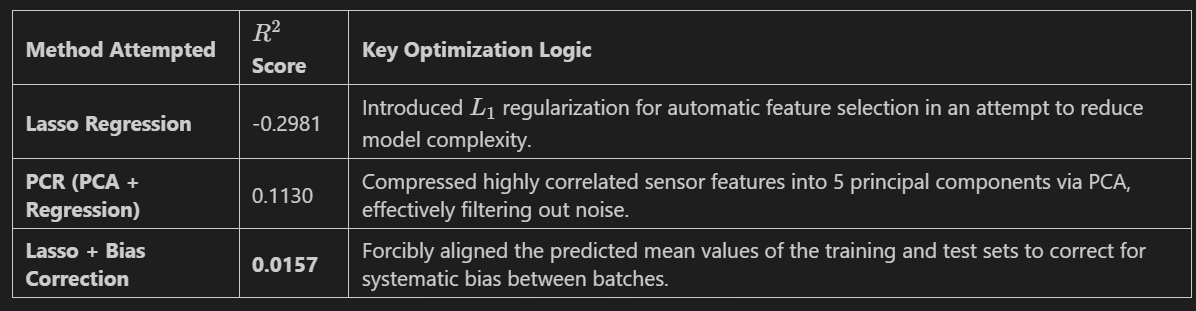
\includegraphics{MDS_Assignment2_313652018_Wang_Xuan-Wei_files/image.png}
\caption{Performance}
\end{figure}

    Discussion: CART vs.~Random Forest vs.~GBDT * Ensemble Effectiveness
(Boosting vs.~Bagging): * \textbf{Random Forest} (0.7375 AUC)
outperforms GBDT (0.6753 AUC) on the balanced dataset. * Insight: In the
noisy SECOM environment, Random Forest's \textbf{``Voting'' mechanism
(Bagging) is more robust} against SMOTE-generated noise than GBDT's
``Error Correction'' (Boosting) approach.

\begin{itemize}
\tightlist
\item
  Learning Mechanism:

  \begin{itemize}
  \tightlist
  \item
    GBDT focuses on correcting residuals (errors). While it successfully
    increased the F1-score (0.10), the drop in ROC AUC suggests it might
    be over-fitting to the synthetic samples created by SMOTE,
    \textbf{struggling to maintain a clear global boundary}.
  \end{itemize}
\end{itemize}

    \begin{itemize}
\tightlist
\item
  Final Recommendation:

  \begin{itemize}
  \tightlist
  \item
    For the SECOM dataset, \textbf{\emph{Random Forest}} remains the
    \emph{most reliable model due to its stability with imbalanced data
    and SMOTE.} However, GBDT's ability to boost the F1-score suggests
    it could be powerful if combined with stricter Feature Selection to
    remove overlapping noise before training.
  \end{itemize}
\end{itemize}

    \section{Process Performance Prediction and Health Status
Analysis}\label{process-performance-prediction-and-health-status-analysis}

    \begin{tcolorbox}[breakable, size=fbox, boxrule=1pt, pad at break*=1mm,colback=cellbackground, colframe=cellborder]
\prompt{In}{incolor}{3}{\boxspacing}
\begin{Verbatim}[commandchars=\\\{\}]
\PY{k+kn}{import}\PY{+w}{ }\PY{n+nn}{seaborn}\PY{+w}{ }\PY{k}{as}\PY{+w}{ }\PY{n+nn}{sns}

\PY{n}{file\PYZus{}path} \PY{o}{=} \PY{l+s+s1}{\PYZsq{}}\PY{l+s+s1}{CMP\PYZhy{}training\PYZhy{}removalrate.csv}\PY{l+s+s1}{\PYZsq{}}
\PY{n}{df} \PY{o}{=} \PY{n}{pd}\PY{o}{.}\PY{n}{read\PYZus{}csv}\PY{p}{(}\PY{n}{file\PYZus{}path}\PY{p}{)}

\PY{n}{sns}\PY{o}{.}\PY{n}{set}\PY{p}{(}\PY{n}{style}\PY{o}{=}\PY{l+s+s2}{\PYZdq{}}\PY{l+s+s2}{whitegrid}\PY{l+s+s2}{\PYZdq{}}\PY{p}{,} \PY{n}{font\PYZus{}scale}\PY{o}{=}\PY{l+m+mf}{1.2}\PY{p}{)}

\PY{n+nb}{print}\PY{p}{(}\PY{l+s+s2}{\PYZdq{}}\PY{l+s+s2}{\PYZhy{}\PYZhy{}\PYZhy{} 1. Data summary \PYZhy{}\PYZhy{}\PYZhy{}}\PY{l+s+s2}{\PYZdq{}}\PY{p}{)}
\PY{n+nb}{print}\PY{p}{(}\PY{l+s+sa}{f}\PY{l+s+s2}{\PYZdq{}}\PY{l+s+s2}{Sample numbers: }\PY{l+s+si}{\PYZob{}}\PY{n+nb}{len}\PY{p}{(}\PY{n}{df}\PY{p}{)}\PY{l+s+si}{\PYZcb{}}\PY{l+s+s2}{\PYZdq{}}\PY{p}{)}
\PY{n+nb}{print}\PY{p}{(}\PY{l+s+sa}{f}\PY{l+s+s2}{\PYZdq{}}\PY{l+s+s2}{Feature columns: }\PY{l+s+si}{\PYZob{}}\PY{n}{df}\PY{o}{.}\PY{n}{columns}\PY{o}{.}\PY{n}{tolist}\PY{p}{(}\PY{p}{)}\PY{l+s+si}{\PYZcb{}}\PY{l+s+s2}{\PYZdq{}}\PY{p}{)}
\PY{n+nb}{print}\PY{p}{(}\PY{l+s+sa}{f}\PY{l+s+s2}{\PYZdq{}}\PY{l+s+s2}{Number of input variables: 25 (Sensor variables)}\PY{l+s+s2}{\PYZdq{}}\PY{p}{)}
\PY{n+nb}{print}\PY{p}{(}\PY{l+s+sa}{f}\PY{l+s+s2}{\PYZdq{}}\PY{l+s+s2}{Target variable: AVG\PYZus{}REMOVAL\PYZus{}RATE}\PY{l+s+s2}{\PYZdq{}}\PY{p}{)}
\PY{n+nb}{print}\PY{p}{(}\PY{l+s+s2}{\PYZdq{}}\PY{l+s+s2}{\PYZhy{}}\PY{l+s+s2}{\PYZdq{}} \PY{o}{*} \PY{l+m+mi}{30} \PY{o}{+} \PY{l+s+s2}{\PYZdq{}}\PY{l+s+se}{\PYZbs{}n}\PY{l+s+s2}{\PYZdq{}}\PY{p}{)}

\PY{n+nb}{print}\PY{p}{(}\PY{l+s+s2}{\PYZdq{}}\PY{l+s+s2}{\PYZhy{}\PYZhy{}\PYZhy{} 2. Target variable statistics \PYZhy{}\PYZhy{}\PYZhy{}}\PY{l+s+s2}{\PYZdq{}}\PY{p}{)}
\PY{n}{stats} \PY{o}{=} \PY{n}{df}\PY{p}{[}\PY{l+s+s1}{\PYZsq{}}\PY{l+s+s1}{AVG\PYZus{}REMOVAL\PYZus{}RATE}\PY{l+s+s1}{\PYZsq{}}\PY{p}{]}\PY{o}{.}\PY{n}{describe}\PY{p}{(}\PY{p}{)}
\PY{n+nb}{print}\PY{p}{(}\PY{n}{stats}\PY{p}{)}
\PY{n+nb}{print}\PY{p}{(}\PY{l+s+s2}{\PYZdq{}}\PY{l+s+s2}{\PYZhy{}}\PY{l+s+s2}{\PYZdq{}} \PY{o}{*} \PY{l+m+mi}{30} \PY{o}{+} \PY{l+s+s2}{\PYZdq{}}\PY{l+s+se}{\PYZbs{}n}\PY{l+s+s2}{\PYZdq{}}\PY{p}{)}

\PY{n+nb}{print}\PY{p}{(}\PY{l+s+s2}{\PYZdq{}}\PY{l+s+s2}{\PYZhy{}\PYZhy{}\PYZhy{} 3. Stage Statistics \PYZhy{}\PYZhy{}\PYZhy{}}\PY{l+s+s2}{\PYZdq{}}\PY{p}{)}
\PY{n}{stage\PYZus{}stats} \PY{o}{=} \PY{n}{df}\PY{o}{.}\PY{n}{groupby}\PY{p}{(}\PY{l+s+s1}{\PYZsq{}}\PY{l+s+s1}{STAGE}\PY{l+s+s1}{\PYZsq{}}\PY{p}{)}\PY{p}{[}\PY{l+s+s1}{\PYZsq{}}\PY{l+s+s1}{AVG\PYZus{}REMOVAL\PYZus{}RATE}\PY{l+s+s1}{\PYZsq{}}\PY{p}{]}\PY{o}{.}\PY{n}{describe}\PY{p}{(}\PY{p}{)}
\PY{n+nb}{print}\PY{p}{(}\PY{n}{stage\PYZus{}stats}\PY{p}{)}
\PY{n+nb}{print}\PY{p}{(}\PY{l+s+s2}{\PYZdq{}}\PY{l+s+s2}{\PYZhy{}}\PY{l+s+s2}{\PYZdq{}} \PY{o}{*} \PY{l+m+mi}{30} \PY{o}{+} \PY{l+s+s2}{\PYZdq{}}\PY{l+s+se}{\PYZbs{}n}\PY{l+s+s2}{\PYZdq{}}\PY{p}{)}
\end{Verbatim}
\end{tcolorbox}

    \begin{Verbatim}[commandchars=\\\{\}]
--- 1. Data summary ---
Sample numbers: 1981
Feature columns: ['WAFER\_ID', 'STAGE', 'AVG\_REMOVAL\_RATE']
Number of input variables: 25 (Sensor variables)
Target variable: AVG\_REMOVAL\_RATE
------------------------------

--- 2. Target variable statistics ---
count    1981.000000
mean       98.631645
std       187.429160
min        53.426550
25\%        72.376500
50\%        79.154850
75\%        88.702050
max      4326.154050
Name: AVG\_REMOVAL\_RATE, dtype: float64
------------------------------

--- 3. Stage Statistics ---
        count        mean         std       min        25\%       50\%  \textbackslash{}
STAGE
A      1166.0  111.674864  243.378343  53.42655  71.894137  77.34585
B       815.0   79.971039    9.150406  54.30720  73.326375  81.51060

             75\%         max
STAGE
A      148.03755  4326.15405
B       86.75595   101.46480
------------------------------

    \end{Verbatim}

    \subsection{Data Science Framework}\label{data-science-framework}

\begin{figure}
\centering
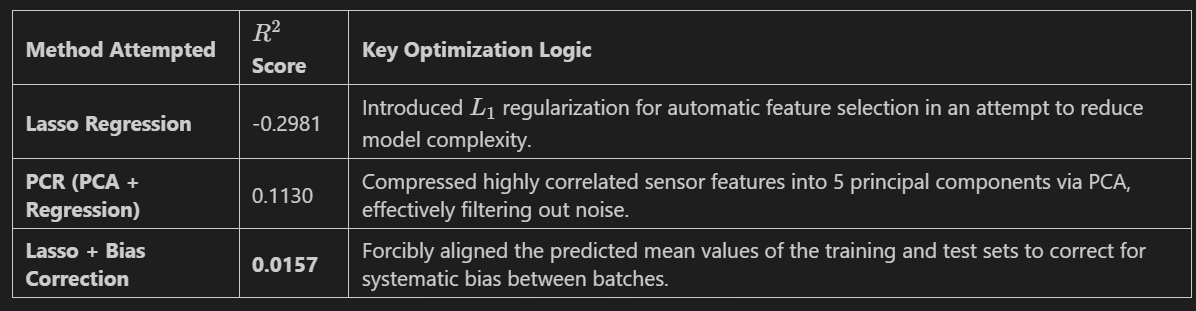
\includegraphics{MDS_Assignment2_313652018_Wang_Xuan-Wei_files/image.png}
\caption{2.1\_dataScienceFramework}
\end{figure}

    Based on the statistical analysis of the label file
\texttt{training\_removalrate.csv} and the associated sensor data files,
the preliminary data summary is provided below:

\subsubsection{Sample Scale and Feature
Dimensions}\label{sample-scale-and-feature-dimensions}

\begin{itemize}
\tightlist
\item
  Total Sample Size: 1,981 observations
\item
  Feature Count:

  \begin{itemize}
  \tightlist
  \item
    Input Features (X): 25 process and equipment-related variables

    \begin{itemize}
    \tightlist
    \item
      e.g., Chamber Pressure, Slurry Flow Rate, Table Speed, and
      Consumable Usage.
    \end{itemize}
  \item
    Target Variable (Y): \texttt{AVG\_REMOVAL\_RATE}, a continuous
    numerical value representing the material removal performance.
  \end{itemize}
\item
  Data Structure: The raw sensor data consists of \textbf{high-frequency
  time-series signals (1 Hz)}. These signals are transformed into
  fixed-dimensional feature vectors through feature engineering (e.g.,
  aggregating via Mean and Standard Deviation).
\end{itemize}

\subsubsection{Distribution Across Process Stages (STAGE A \&
B)}\label{distribution-across-process-stages-stage-a-b}

The analysis reveals significant physical and performance differences
between the two stages: * \textbf{Stage A (Primary Polishing)}: * Sample
Count: \textbf{1,166} entries. * Mean Removal Rate: \textbf{111.67}
(significantly higher than Stage B), indicating aggressive material
removal. * Variability: A high standard deviation of \textbf{243.38}
with extreme outliers (Max: 4326.15), suggesting a more volatile process
environment. * \textbf{Stage B (Final Buffing/Stabilization)}: * Sample
Count: 815 entries. * Mean Removal Rate: 79.97, with a highly
concentrated distribution. * Stability: A low standard deviation of
\textbf{9.15}, with values strictly ranging between 54 and 101,
indicating high process stability.

\subsubsection{Statistical Characteristics of Target Variable
(AVG\_REMOVAL\_RATE)}\label{statistical-characteristics-of-target-variable-avg_removal_rate}

\begin{itemize}
\tightlist
\item
  \textbf{Central Tendency}: The global mean is \textbf{98.63}, while
  the median is \textbf{79.15}. The fact that the mean is significantly
  higher than the median confirms a \textbf{highly right-skewed}
  distribution.
\item
  \textbf{Dispersion}: The overall standard deviation is
  \textbf{187.43}, reflecting high cross-batch and cross-stage variance.
\item
  \textbf{Outlier Observation}:

  \begin{itemize}
  \tightlist
  \item
    \textbf{Minimum}: 53.43.
  \item
    \textbf{Maximum}: \textbf{4326.15}.
  \item
    \textbf{Insights}: The extreme gap between the 75th percentile
    (88.7) and the maximum value confirms the presence of
    \textbf{extreme outliers}.
  \end{itemize}
\end{itemize}

    \subsection{Data Quality Inspection and
Preprocessing}\label{data-quality-inspection-and-preprocessing}

    We aggregate all the training files by following steps: 1. Using
\texttt{glob} catch all the 185 files, and mark the empty files 2.
Calculating the \textbf{Mean} (representing the process level) and
\textbf{Standard Deviation} (capturing process stability and equipment
vibration) for all 25 sensor variables. 3. Applying \texttt{unstack}
method to flatten the statistics into a single-row feature vector 4.
Label-integrating with ``CMP-training-removalrate.csv'' file, with
``WAFER\_ID'' and ``STAGE'' as the primary keys.

    \begin{tcolorbox}[breakable, size=fbox, boxrule=1pt, pad at break*=1mm,colback=cellbackground, colframe=cellborder]
\prompt{In}{incolor}{ }{\boxspacing}
\begin{Verbatim}[commandchars=\\\{\}]
\PY{k+kn}{import}\PY{+w}{ }\PY{n+nn}{pandas}\PY{+w}{ }\PY{k}{as}\PY{+w}{ }\PY{n+nn}{pd}
\PY{k+kn}{import}\PY{+w}{ }\PY{n+nn}{glob}
\PY{k+kn}{import}\PY{+w}{ }\PY{n+nn}{os}

\PY{n}{base\PYZus{}path} \PY{o}{=} \PY{l+s+sa}{r}\PY{l+s+s2}{\PYZdq{}}\PY{l+s+s2}{C:}\PY{l+s+s2}{\PYZbs{}}\PY{l+s+s2}{Users}\PY{l+s+s2}{\PYZbs{}}\PY{l+s+s2}{user}\PY{l+s+s2}{\PYZbs{}}\PY{l+s+s2}{OneDrive \PYZhy{} 國立陽明交通大學}\PY{l+s+s2}{\PYZbs{}}\PY{l+s+s2}{桌面}\PY{l+s+s2}{\PYZbs{}}\PY{l+s+s2}{001\PYZus{}\PYZus{}1142碩士生存指南}\PY{l+s+s2}{\PYZbs{}}\PY{l+s+s2}{536907\PYZus{}製造數據科學\PYZus{}洪佑鑫}\PY{l+s+s2}{\PYZbs{}}\PY{l+s+s2}{1142MDS\PYZus{}Project\PYZus{}313652018\PYZus{}Xuan\PYZhy{}Wei\PYZhy{}Wang}\PY{l+s+s2}{\PYZbs{}}\PY{l+s+s2}{Assignment02}\PY{l+s+s2}{\PYZbs{}}\PY{l+s+s2}{2016 PHM Data Challenge}\PY{l+s+s2}{\PYZbs{}}\PY{l+s+s2}{2016 PHM DATA CHALLENGE CMP DATA SET}\PY{l+s+s2}{\PYZbs{}}\PY{l+s+s2}{CMP\PYZhy{}data}\PY{l+s+s2}{\PYZdq{}}
\PY{n}{training\PYZus{}data\PYZus{}path} \PY{o}{=} \PY{n}{os}\PY{o}{.}\PY{n}{path}\PY{o}{.}\PY{n}{join}\PY{p}{(}\PY{n}{base\PYZus{}path}\PY{p}{,} \PY{l+s+s2}{\PYZdq{}}\PY{l+s+s2}{training}\PY{l+s+s2}{\PYZdq{}}\PY{p}{)}
\PY{n}{label\PYZus{}file} \PY{o}{=} \PY{n}{os}\PY{o}{.}\PY{n}{path}\PY{o}{.}\PY{n}{join}\PY{p}{(}\PY{n}{base\PYZus{}path}\PY{p}{,} \PY{l+s+s2}{\PYZdq{}}\PY{l+s+s2}{CMP\PYZhy{}training\PYZhy{}removalrate.csv}\PY{l+s+s2}{\PYZdq{}}\PY{p}{)}

\PY{n}{file\PYZus{}list} \PY{o}{=} \PY{n}{glob}\PY{o}{.}\PY{n}{glob}\PY{p}{(}\PY{n}{os}\PY{o}{.}\PY{n}{path}\PY{o}{.}\PY{n}{join}\PY{p}{(}\PY{n}{training\PYZus{}data\PYZus{}path}\PY{p}{,} \PY{l+s+s2}{\PYZdq{}}\PY{l+s+s2}{*.csv}\PY{l+s+s2}{\PYZdq{}}\PY{p}{)}\PY{p}{)}
\PY{n+nb}{print}\PY{p}{(}\PY{l+s+sa}{f}\PY{l+s+s2}{\PYZdq{}}\PY{l+s+s2}{Find }\PY{l+s+si}{\PYZob{}}\PY{n+nb}{len}\PY{p}{(}\PY{n}{file\PYZus{}list}\PY{p}{)}\PY{l+s+si}{\PYZcb{}}\PY{l+s+s2}{ sensor files, about to aggregate...}\PY{l+s+s2}{\PYZdq{}}\PY{p}{)}
\PY{n}{summary\PYZus{}list} \PY{o}{=} \PY{p}{[}\PY{p}{]}
\PY{k}{for} \PY{n}{i}\PY{p}{,} \PY{n}{file} \PY{o+ow}{in} \PY{n+nb}{enumerate}\PY{p}{(}\PY{n}{file\PYZus{}list}\PY{p}{)}\PY{p}{:}
    \PY{n}{temp\PYZus{}df} \PY{o}{=} \PY{n}{pd}\PY{o}{.}\PY{n}{read\PYZus{}csv}\PY{p}{(}\PY{n}{file}\PY{p}{)}
    
    \PY{k}{if} \PY{n}{temp\PYZus{}df}\PY{o}{.}\PY{n}{empty}\PY{p}{:}
        \PY{k}{continue}
        
    \PY{k}{try}\PY{p}{:}
        \PY{n}{wafer\PYZus{}id} \PY{o}{=} \PY{n+nb}{str}\PY{p}{(}\PY{n}{temp\PYZus{}df}\PY{p}{[}\PY{l+s+s1}{\PYZsq{}}\PY{l+s+s1}{WAFER\PYZus{}ID}\PY{l+s+s1}{\PYZsq{}}\PY{p}{]}\PY{o}{.}\PY{n}{iloc}\PY{p}{[}\PY{l+m+mi}{0}\PY{p}{]}\PY{p}{)}
        \PY{n}{stage} \PY{o}{=} \PY{n+nb}{str}\PY{p}{(}\PY{n}{temp\PYZus{}df}\PY{p}{[}\PY{l+s+s1}{\PYZsq{}}\PY{l+s+s1}{STAGE}\PY{l+s+s1}{\PYZsq{}}\PY{p}{]}\PY{o}{.}\PY{n}{iloc}\PY{p}{[}\PY{l+m+mi}{0}\PY{p}{]}\PY{p}{)}
        \PY{n}{chamber\PYZus{}val} \PY{o}{=} \PY{n+nb}{int}\PY{p}{(}\PY{n}{temp\PYZus{}df}\PY{p}{[}\PY{l+s+s1}{\PYZsq{}}\PY{l+s+s1}{CHAMBER}\PY{l+s+s1}{\PYZsq{}}\PY{p}{]}\PY{o}{.}\PY{n}{iloc}\PY{p}{[}\PY{l+m+mi}{0}\PY{p}{]}\PY{p}{)}
        \PY{n}{stage\PYZus{}chamber\PYZus{}key} \PY{o}{=} \PY{l+s+sa}{f}\PY{l+s+s2}{\PYZdq{}}\PY{l+s+si}{\PYZob{}}\PY{n}{stage}\PY{l+s+si}{\PYZcb{}}\PY{l+s+s2}{\PYZus{}}\PY{l+s+si}{\PYZob{}}\PY{n}{chamber\PYZus{}val}\PY{l+s+si}{\PYZcb{}}\PY{l+s+s2}{\PYZdq{}}
        
        \PY{n}{cols\PYZus{}to\PYZus{}drop} \PY{o}{=} \PY{p}{[}\PY{l+s+s1}{\PYZsq{}}\PY{l+s+s1}{WAFER\PYZus{}ID}\PY{l+s+s1}{\PYZsq{}}\PY{p}{,} \PY{l+s+s1}{\PYZsq{}}\PY{l+s+s1}{STAGE}\PY{l+s+s1}{\PYZsq{}}\PY{p}{,} \PY{l+s+s1}{\PYZsq{}}\PY{l+s+s1}{CHAMBER}\PY{l+s+s1}{\PYZsq{}}\PY{p}{,} \PY{l+s+s1}{\PYZsq{}}\PY{l+s+s1}{TIMESTAMP}\PY{l+s+s1}{\PYZsq{}}\PY{p}{,} \PY{l+s+s1}{\PYZsq{}}\PY{l+s+s1}{MACHINE\PYZus{}ID}\PY{l+s+s1}{\PYZsq{}}\PY{p}{,} \PY{l+s+s1}{\PYZsq{}}\PY{l+s+s1}{MACHINE\PYZus{}DATA}\PY{l+s+s1}{\PYZsq{}}\PY{p}{]}
        \PY{n}{numeric\PYZus{}features} \PY{o}{=} \PY{n}{temp\PYZus{}df}\PY{o}{.}\PY{n}{select\PYZus{}dtypes}\PY{p}{(}\PY{n}{include}\PY{o}{=}\PY{p}{[}\PY{l+s+s1}{\PYZsq{}}\PY{l+s+s1}{number}\PY{l+s+s1}{\PYZsq{}}\PY{p}{]}\PY{p}{)}\PY{o}{.}\PY{n}{drop}\PY{p}{(}\PY{n}{columns}\PY{o}{=}\PY{p}{[}\PY{n}{c} \PY{k}{for} \PY{n}{col} \PY{o+ow}{in} \PY{n}{temp\PYZus{}df}\PY{o}{.}\PY{n}{columns} \PY{k}{for} \PY{n}{c} \PY{o+ow}{in} \PY{n}{cols\PYZus{}to\PYZus{}drop} \PY{k}{if} \PY{n}{col} \PY{o}{==} \PY{n}{c}\PY{p}{]}\PY{p}{,} \PY{n}{errors}\PY{o}{=}\PY{l+s+s1}{\PYZsq{}}\PY{l+s+s1}{ignore}\PY{l+s+s1}{\PYZsq{}}\PY{p}{)}
        
        \PY{n}{stats} \PY{o}{=} \PY{n}{numeric\PYZus{}features}\PY{o}{.}\PY{n}{agg}\PY{p}{(}\PY{p}{[}\PY{l+s+s1}{\PYZsq{}}\PY{l+s+s1}{mean}\PY{l+s+s1}{\PYZsq{}}\PY{p}{,} \PY{l+s+s1}{\PYZsq{}}\PY{l+s+s1}{std}\PY{l+s+s1}{\PYZsq{}}\PY{p}{]}\PY{p}{)}
        
        \PY{n}{row\PYZus{}stats} \PY{o}{=} \PY{n}{stats}\PY{o}{.}\PY{n}{unstack}\PY{p}{(}\PY{p}{)}\PY{o}{.}\PY{n}{to\PYZus{}frame}\PY{p}{(}\PY{p}{)}\PY{o}{.}\PY{n}{T}
        \PY{n}{row\PYZus{}stats}\PY{o}{.}\PY{n}{columns} \PY{o}{=} \PY{p}{[}\PY{l+s+sa}{f}\PY{l+s+s1}{\PYZsq{}}\PY{l+s+si}{\PYZob{}}\PY{n}{col}\PY{p}{[}\PY{l+m+mi}{0}\PY{p}{]}\PY{l+s+si}{\PYZcb{}}\PY{l+s+s1}{\PYZus{}}\PY{l+s+si}{\PYZob{}}\PY{n}{col}\PY{p}{[}\PY{l+m+mi}{1}\PY{p}{]}\PY{l+s+si}{\PYZcb{}}\PY{l+s+s1}{\PYZsq{}} \PY{k}{for} \PY{n}{col} \PY{o+ow}{in} \PY{n}{row\PYZus{}stats}\PY{o}{.}\PY{n}{columns}\PY{p}{]}
        
        \PY{n}{row\PYZus{}stats}\PY{p}{[}\PY{l+s+s1}{\PYZsq{}}\PY{l+s+s1}{Process\PYZus{}Duration}\PY{l+s+s1}{\PYZsq{}}\PY{p}{]} \PY{o}{=} \PY{n+nb}{len}\PY{p}{(}\PY{n}{temp\PYZus{}df}\PY{p}{)}
        \PY{n}{row\PYZus{}stats}\PY{p}{[}\PY{l+s+s1}{\PYZsq{}}\PY{l+s+s1}{WAFER\PYZus{}ID}\PY{l+s+s1}{\PYZsq{}}\PY{p}{]} \PY{o}{=} \PY{n}{wafer\PYZus{}id}
        \PY{n}{row\PYZus{}stats}\PY{p}{[}\PY{l+s+s1}{\PYZsq{}}\PY{l+s+s1}{STAGE}\PY{l+s+s1}{\PYZsq{}}\PY{p}{]} \PY{o}{=} \PY{n}{stage}
        \PY{n}{row\PYZus{}stats}\PY{p}{[}\PY{l+s+s1}{\PYZsq{}}\PY{l+s+s1}{CHAMBER}\PY{l+s+s1}{\PYZsq{}}\PY{p}{]} \PY{o}{=} \PY{n}{chamber\PYZus{}val}
        \PY{n}{row\PYZus{}stats}\PY{p}{[}\PY{l+s+s1}{\PYZsq{}}\PY{l+s+s1}{STAGE\PYZus{}CHAMBER}\PY{l+s+s1}{\PYZsq{}}\PY{p}{]} \PY{o}{=} \PY{n}{stage\PYZus{}chamber\PYZus{}key} 
        \PY{n}{summary\PYZus{}list}\PY{o}{.}\PY{n}{append}\PY{p}{(}\PY{n}{row\PYZus{}stats}\PY{p}{)}
        
    \PY{k}{except} \PY{n+ne}{Exception} \PY{k}{as} \PY{n}{e}\PY{p}{:}
        \PY{n+nb}{print}\PY{p}{(}\PY{l+s+sa}{f}\PY{l+s+s2}{\PYZdq{}}\PY{l+s+s2}{\PYZgt{}\PYZgt{}\PYZgt{}\PYZgt{}\PYZgt{}\PYZgt{} ERROR: File }\PY{l+s+si}{\PYZob{}}\PY{n}{os}\PY{o}{.}\PY{n}{path}\PY{o}{.}\PY{n}{basename}\PY{p}{(}\PY{n}{file}\PY{p}{)}\PY{l+s+si}{\PYZcb{}}\PY{l+s+s2}{ is invalid: }\PY{l+s+si}{\PYZob{}}\PY{n+nb}{str}\PY{p}{(}\PY{n}{e}\PY{p}{)}\PY{l+s+si}{\PYZcb{}}\PY{l+s+s2}{\PYZdq{}}\PY{p}{)}
        \PY{k}{continue}

    \PY{k}{if} \PY{p}{(}\PY{n}{i}\PY{o}{+}\PY{l+m+mi}{1}\PY{p}{)} \PY{o}{\PYZpc{}} \PY{l+m+mi}{50} \PY{o}{==} \PY{l+m+mi}{0}\PY{p}{:}
        \PY{n+nb}{print}\PY{p}{(}\PY{l+s+sa}{f}\PY{l+s+s2}{\PYZdq{}}\PY{l+s+s2}{====== PROGRESS: Processed }\PY{l+s+si}{\PYZob{}}\PY{n}{i}\PY{o}{+}\PY{l+m+mi}{1}\PY{l+s+si}{\PYZcb{}}\PY{l+s+s2}{ files...}\PY{l+s+s2}{\PYZdq{}}\PY{p}{)} 

\PY{n}{df\PYZus{}features} \PY{o}{=} \PY{n}{pd}\PY{o}{.}\PY{n}{concat}\PY{p}{(}\PY{n}{summary\PYZus{}list}\PY{p}{,} \PY{n}{ignore\PYZus{}index}\PY{o}{=}\PY{k+kc}{True}\PY{p}{)}
\PY{n}{labels} \PY{o}{=} \PY{n}{pd}\PY{o}{.}\PY{n}{read\PYZus{}csv}\PY{p}{(}\PY{n}{label\PYZus{}file}\PY{p}{)}
\PY{n}{labels}\PY{p}{[}\PY{l+s+s1}{\PYZsq{}}\PY{l+s+s1}{WAFER\PYZus{}ID}\PY{l+s+s1}{\PYZsq{}}\PY{p}{]} \PY{o}{=} \PY{n}{labels}\PY{p}{[}\PY{l+s+s1}{\PYZsq{}}\PY{l+s+s1}{WAFER\PYZus{}ID}\PY{l+s+s1}{\PYZsq{}}\PY{p}{]}\PY{o}{.}\PY{n}{astype}\PY{p}{(}\PY{n+nb}{str}\PY{p}{)}
\PY{n}{labels}\PY{p}{[}\PY{l+s+s1}{\PYZsq{}}\PY{l+s+s1}{STAGE}\PY{l+s+s1}{\PYZsq{}}\PY{p}{]} \PY{o}{=} \PY{n}{labels}\PY{p}{[}\PY{l+s+s1}{\PYZsq{}}\PY{l+s+s1}{STAGE}\PY{l+s+s1}{\PYZsq{}}\PY{p}{]}\PY{o}{.}\PY{n}{astype}\PY{p}{(}\PY{n+nb}{str}\PY{p}{)}

\PY{n}{df\PYZus{}final} \PY{o}{=} \PY{n}{pd}\PY{o}{.}\PY{n}{merge}\PY{p}{(}\PY{n}{df\PYZus{}features}\PY{p}{,} \PY{n}{labels}\PY{p}{,} \PY{n}{on}\PY{o}{=}\PY{p}{[}\PY{l+s+s1}{\PYZsq{}}\PY{l+s+s1}{WAFER\PYZus{}ID}\PY{l+s+s1}{\PYZsq{}}\PY{p}{,} \PY{l+s+s1}{\PYZsq{}}\PY{l+s+s1}{STAGE}\PY{l+s+s1}{\PYZsq{}}\PY{p}{]}\PY{p}{,} \PY{n}{how}\PY{o}{=}\PY{l+s+s1}{\PYZsq{}}\PY{l+s+s1}{inner}\PY{l+s+s1}{\PYZsq{}}\PY{p}{)}

\PY{n+nb}{print}\PY{p}{(}\PY{l+s+s2}{\PYZdq{}}\PY{l+s+se}{\PYZbs{}n}\PY{l+s+s2}{===\PYZgt{}\PYZgt{}\PYZgt{}\PYZgt{}\PYZgt{} SUCCESS: Data aggregation complete!\PYZlt{}\PYZlt{}\PYZlt{}\PYZlt{}\PYZlt{}\PYZlt{}===}\PY{l+s+s2}{\PYZdq{}}\PY{p}{)}
\PY{n+nb}{print}\PY{p}{(}\PY{l+s+sa}{f}\PY{l+s+s2}{\PYZdq{}}\PY{l+s+s2}{Final feature matrix shape: }\PY{l+s+si}{\PYZob{}}\PY{n}{df\PYZus{}final}\PY{o}{.}\PY{n}{shape}\PY{l+s+si}{\PYZcb{}}\PY{l+s+s2}{\PYZdq{}}\PY{p}{)}

\PY{k}{if} \PY{l+s+s1}{\PYZsq{}}\PY{l+s+s1}{STAGE\PYZus{}CHAMBER}\PY{l+s+s1}{\PYZsq{}} \PY{o+ow}{in} \PY{n}{df\PYZus{}final}\PY{o}{.}\PY{n}{columns}\PY{p}{:}
    \PY{n+nb}{print}\PY{p}{(}\PY{l+s+s2}{\PYZdq{}}\PY{l+s+se}{\PYZbs{}n}\PY{l+s+s2}{[2.3 EDA Diagnosis Tip] Mean Removal Rate by Stage\PYZus{}Chamber:}\PY{l+s+s2}{\PYZdq{}}\PY{p}{)}
    \PY{n+nb}{print}\PY{p}{(}\PY{n}{df\PYZus{}final}\PY{o}{.}\PY{n}{groupby}\PY{p}{(}\PY{l+s+s1}{\PYZsq{}}\PY{l+s+s1}{STAGE\PYZus{}CHAMBER}\PY{l+s+s1}{\PYZsq{}}\PY{p}{)}\PY{p}{[}\PY{l+s+s1}{\PYZsq{}}\PY{l+s+s1}{AVG\PYZus{}REMOVAL\PYZus{}RATE}\PY{l+s+s1}{\PYZsq{}}\PY{p}{]}\PY{o}{.}\PY{n}{mean}\PY{p}{(}\PY{p}{)}\PY{o}{.}\PY{n}{sort\PYZus{}values}\PY{p}{(}\PY{n}{ascending}\PY{o}{=}\PY{k+kc}{False}\PY{p}{)}\PY{p}{)}

\PY{n}{df\PYZus{}final}\PY{o}{.}\PY{n}{head}\PY{p}{(}\PY{p}{)}
\end{Verbatim}
\end{tcolorbox}

    \begin{Verbatim}[commandchars=\\\{\}]
Find 185 sensor files, about to aggregate{\ldots}
====== PROGRESS: Processed 50 files{\ldots}
====== PROGRESS: Processed 100 files{\ldots}
====== PROGRESS: Processed 150 files{\ldots}

===>>>>> SUCCESS: Data aggregation complete!<<<<<<===
Final feature matrix shape: (184, 44)

[2.3 EDA Diagnosis Tip] Mean Removal Rate by Stage\_Chamber:
STAGE\_CHAMBER
A\_1    188.713229
B\_4     81.091557
A\_4     73.252905
Name: AVG\_REMOVAL\_RATE, dtype: float64
    \end{Verbatim}

            \begin{tcolorbox}[breakable, size=fbox, boxrule=.5pt, pad at break*=1mm, opacityfill=0]
\prompt{Out}{outcolor}{ }{\boxspacing}
\begin{Verbatim}[commandchars=\\\{\}]
   USAGE\_OF\_BACKING\_FILM\_mean  USAGE\_OF\_BACKING\_FILM\_std  \textbackslash{}
0                 9338.075348                  80.511031
1                 9703.238113                  86.864677
2                 9991.971483                  96.929373
3                 2972.610931                4537.516981
4                  418.110632                  89.717660

   USAGE\_OF\_DRESSER\_mean  USAGE\_OF\_DRESSER\_std  USAGE\_OF\_POLISHING\_TABLE\_mean  \textbackslash{}
0             536.057573              4.722434                     251.504029
1             555.676669              3.804677                     236.174626
2             572.558344              4.283878                     127.033832
3             593.001318              4.288880                     171.553078
4             609.219440              4.669346                     125.133370

   USAGE\_OF\_POLISHING\_TABLE\_std  USAGE\_OF\_DRESSER\_TABLE\_mean  \textbackslash{}
0                     89.195353                  2667.598963
1                     77.198713                  2680.840584
2                     84.162334                  2692.247485
3                     91.691896                  2706.046090
4                     79.775997                  2716.988978

   USAGE\_OF\_DRESSER\_TABLE\_std  PRESSURIZED\_CHAMBER\_PRESSURE\_mean  \textbackslash{}
0                    3.184136                          52.752363
1                    2.578330                          58.225718
2                    2.883222                          57.107475
3                    2.905676                          54.466533
4                    3.133999                          51.863476

   PRESSURIZED\_CHAMBER\_PRESSURE\_std  {\ldots}  DRESSING\_WATER\_STATUS\_mean  \textbackslash{}
0                         40.698930  {\ldots}                    0.542452
1                         34.741006  {\ldots}                    0.328698
2                         40.485907  {\ldots}                    0.454467
3                         36.707887  {\ldots}                    0.501942
4                         36.692925  {\ldots}                    0.426232

   DRESSING\_WATER\_STATUS\_std  EDGE\_AIR\_BAG\_PRESSURE\_mean  \textbackslash{}
0                   0.498263                   30.924644
1                   0.469784                   34.128126
2                   0.497949                   32.430797
3                   0.500023                   31.256611
4                   0.494559                   29.660509

   EDGE\_AIR\_BAG\_PRESSURE\_std  Process\_Duration    WAFER\_ID  STAGE  CHAMBER  \textbackslash{}
0                  25.202157              3663   371447024      A        1
1                  22.388594              5321  -875170052      B        4
2                  24.865236              9246   371447032      A        1
3                  23.394538              9270   329446704      A        1
4                  22.800634              8120   329446870      A        1

   STAGE\_CHAMBER  AVG\_REMOVAL\_RATE
0            A\_1         149.13090
1            B\_4          65.91045
2            A\_1         149.99265
3            A\_1         147.94095
4            A\_1         147.02025

[5 rows x 44 columns]
\end{Verbatim}
\end{tcolorbox}
        
    The previous table shows that: 1. Each row represents a single
``WAFER\_ID'' and its''STAGE'', and the information indecates the mean
and std for each features during the stage process 2. The table is
184\emph{(43+4) dimension: } Since 066.csv is empty, there are only
185-1=\textbf{184} files * There are 21 features for each wafer process,
and each feature we compute its mean and std; therefore, there are
21\emph{2+1= \textbf{43} features for each process, where 1 represents
the time. } And lables are ``WAFER\_ID'', ``STAGE'', ``CHAMBER'' and
``AVG\_REMOVAL\_RATE''

    During aggregation, it was discovered that the training CSV file 066 was
completely blank.\\
The following checks were performed: 1. Duplicate samples 2. Redundant
columns 3. Missing values 4. Outliers

    \begin{tcolorbox}[breakable, size=fbox, boxrule=1pt, pad at break*=1mm,colback=cellbackground, colframe=cellborder]
\prompt{In}{incolor}{8}{\boxspacing}
\begin{Verbatim}[commandchars=\\\{\}]
\PY{c+c1}{\PYZsh{} Duplicate check}
\PY{n}{total\PYZus{}duplicates} \PY{o}{=} \PY{n}{df\PYZus{}final}\PY{o}{.}\PY{n}{duplicated}\PY{p}{(}\PY{p}{)}\PY{o}{.}\PY{n}{sum}\PY{p}{(}\PY{p}{)}
\PY{n+nb}{print}\PY{p}{(}\PY{l+s+sa}{f}\PY{l+s+s2}{\PYZdq{}}\PY{l+s+s2}{Number of duplicate rows: }\PY{l+s+si}{\PYZob{}}\PY{n}{total\PYZus{}duplicates}\PY{l+s+si}{\PYZcb{}}\PY{l+s+s2}{\PYZdq{}}\PY{p}{)}
\PY{k}{if} \PY{n}{total\PYZus{}duplicates} \PY{o}{\PYZgt{}} \PY{l+m+mi}{0}\PY{p}{:}
    \PY{n+nb}{print}\PY{p}{(}\PY{n}{df\PYZus{}final}\PY{p}{[}\PY{n}{df\PYZus{}final}\PY{o}{.}\PY{n}{duplicated}\PY{p}{(}\PY{p}{)}\PY{p}{]}\PY{p}{)}
    
\PY{n}{constant\PYZus{}cols} \PY{o}{=} \PY{n}{df\PYZus{}final}\PY{o}{.}\PY{n}{columns}\PY{p}{[}\PY{n}{df\PYZus{}final}\PY{o}{.}\PY{n}{nunique}\PY{p}{(}\PY{p}{)} \PY{o}{\PYZlt{}}\PY{o}{=} \PY{l+m+mi}{1}\PY{p}{]}\PY{o}{.}\PY{n}{tolist}\PY{p}{(}\PY{p}{)}
\PY{n+nb}{print}\PY{p}{(}\PY{l+s+sa}{f}\PY{l+s+s2}{\PYZdq{}}\PY{l+s+s2}{Number of constant columns: }\PY{l+s+si}{\PYZob{}}\PY{n+nb}{len}\PY{p}{(}\PY{n}{constant\PYZus{}cols}\PY{p}{)}\PY{l+s+si}{\PYZcb{}}\PY{l+s+s2}{\PYZdq{}}\PY{p}{)}
\PY{n+nb}{print}\PY{p}{(}\PY{l+s+sa}{f}\PY{l+s+s2}{\PYZdq{}}\PY{l+s+s2}{Constant columns: }\PY{l+s+si}{\PYZob{}}\PY{n}{constant\PYZus{}cols}\PY{l+s+si}{\PYZcb{}}\PY{l+s+s2}{\PYZdq{}}\PY{p}{)}

\PY{c+c1}{\PYZsh{} Nan check}
\PY{n}{null\PYZus{}counts} \PY{o}{=} \PY{n}{df\PYZus{}final}\PY{o}{.}\PY{n}{isnull}\PY{p}{(}\PY{p}{)}\PY{o}{.}\PY{n}{sum}\PY{p}{(}\PY{p}{)}\PY{o}{.}\PY{n}{sum}\PY{p}{(}\PY{p}{)}
\PY{n+nb}{print}\PY{p}{(}\PY{l+s+sa}{f}\PY{l+s+s2}{\PYZdq{}}\PY{l+s+s2}{Number of missing values after merging: }\PY{l+s+si}{\PYZob{}}\PY{n}{null\PYZus{}counts}\PY{l+s+si}{\PYZcb{}}\PY{l+s+s2}{\PYZdq{}}\PY{p}{)}

\PY{k+kn}{import}\PY{+w}{ }\PY{n+nn}{matplotlib}\PY{n+nn}{.}\PY{n+nn}{pyplot}\PY{+w}{ }\PY{k}{as}\PY{+w}{ }\PY{n+nn}{plt}
\PY{n}{fig}\PY{p}{,} \PY{n}{axes} \PY{o}{=} \PY{n}{plt}\PY{o}{.}\PY{n}{subplots}\PY{p}{(}\PY{l+m+mi}{1}\PY{p}{,} \PY{l+m+mi}{2}\PY{p}{,} \PY{n}{figsize}\PY{o}{=}\PY{p}{(}\PY{l+m+mi}{12}\PY{p}{,} \PY{l+m+mi}{6}\PY{p}{)}\PY{p}{)}

\PY{c+c1}{\PYZsh{} A. Exploratory Boxplot with Outliers}
\PY{n}{sns}\PY{o}{.}\PY{n}{boxplot}\PY{p}{(}\PY{n}{x}\PY{o}{=}\PY{l+s+s1}{\PYZsq{}}\PY{l+s+s1}{STAGE}\PY{l+s+s1}{\PYZsq{}}\PY{p}{,} \PY{n}{y}\PY{o}{=}\PY{l+s+s1}{\PYZsq{}}\PY{l+s+s1}{AVG\PYZus{}REMOVAL\PYZus{}RATE}\PY{l+s+s1}{\PYZsq{}}\PY{p}{,} \PY{n}{data}\PY{o}{=}\PY{n}{df}\PY{p}{,} \PY{n}{ax}\PY{o}{=}\PY{n}{axes}\PY{p}{[}\PY{l+m+mi}{0}\PY{p}{]}\PY{p}{,} \PY{n}{palette}\PY{o}{=}\PY{l+s+s1}{\PYZsq{}}\PY{l+s+s1}{Set2}\PY{l+s+s1}{\PYZsq{}}\PY{p}{)}
\PY{n}{axes}\PY{p}{[}\PY{l+m+mi}{0}\PY{p}{]}\PY{o}{.}\PY{n}{set\PYZus{}title}\PY{p}{(}\PY{l+s+s1}{\PYZsq{}}\PY{l+s+s1}{Original Removal Rate by STAGE (with Outliers)}\PY{l+s+s1}{\PYZsq{}}\PY{p}{)}
\PY{n}{axes}\PY{p}{[}\PY{l+m+mi}{0}\PY{p}{]}\PY{o}{.}\PY{n}{set\PYZus{}ylabel}\PY{p}{(}\PY{l+s+s1}{\PYZsq{}}\PY{l+s+s1}{Removal Rate}\PY{l+s+s1}{\PYZsq{}}\PY{p}{)}

\PY{c+c1}{\PYZsh{} B. Boxplot with Outliers Removed (Filter Top 5\PYZpc{})}
\PY{n}{q\PYZus{}limit} \PY{o}{=} \PY{n}{df}\PY{p}{[}\PY{l+s+s1}{\PYZsq{}}\PY{l+s+s1}{AVG\PYZus{}REMOVAL\PYZus{}RATE}\PY{l+s+s1}{\PYZsq{}}\PY{p}{]}\PY{o}{.}\PY{n}{quantile}\PY{p}{(}\PY{l+m+mf}{0.95}\PY{p}{)}
\PY{n}{df\PYZus{}filtered} \PY{o}{=} \PY{n}{df}\PY{p}{[}\PY{n}{df}\PY{p}{[}\PY{l+s+s1}{\PYZsq{}}\PY{l+s+s1}{AVG\PYZus{}REMOVAL\PYZus{}RATE}\PY{l+s+s1}{\PYZsq{}}\PY{p}{]} \PY{o}{\PYZlt{}} \PY{n}{q\PYZus{}limit}\PY{p}{]}

\PY{n}{sns}\PY{o}{.}\PY{n}{boxplot}\PY{p}{(}\PY{n}{x}\PY{o}{=}\PY{l+s+s1}{\PYZsq{}}\PY{l+s+s1}{STAGE}\PY{l+s+s1}{\PYZsq{}}\PY{p}{,} \PY{n}{y}\PY{o}{=}\PY{l+s+s1}{\PYZsq{}}\PY{l+s+s1}{AVG\PYZus{}REMOVAL\PYZus{}RATE}\PY{l+s+s1}{\PYZsq{}}\PY{p}{,} \PY{n}{data}\PY{o}{=}\PY{n}{df\PYZus{}filtered}\PY{p}{,} \PY{n}{ax}\PY{o}{=}\PY{n}{axes}\PY{p}{[}\PY{l+m+mi}{1}\PY{p}{]}\PY{p}{,} \PY{n}{palette}\PY{o}{=}\PY{l+s+s1}{\PYZsq{}}\PY{l+s+s1}{Set2}\PY{l+s+s1}{\PYZsq{}}\PY{p}{)}
\PY{n}{axes}\PY{p}{[}\PY{l+m+mi}{1}\PY{p}{]}\PY{o}{.}\PY{n}{set\PYZus{}title}\PY{p}{(}\PY{l+s+s1}{\PYZsq{}}\PY{l+s+s1}{Removal Rate by STAGE (Filtered Top 5}\PY{l+s+s1}{\PYZpc{}}\PY{l+s+s1}{)}\PY{l+s+s1}{\PYZsq{}}\PY{p}{)}
\PY{n}{axes}\PY{p}{[}\PY{l+m+mi}{1}\PY{p}{]}\PY{o}{.}\PY{n}{set\PYZus{}ylabel}\PY{p}{(}\PY{l+s+s1}{\PYZsq{}}\PY{l+s+s1}{Removal Rate}\PY{l+s+s1}{\PYZsq{}}\PY{p}{)}

\PY{n}{plt}\PY{o}{.}\PY{n}{tight\PYZus{}layout}\PY{p}{(}\PY{p}{)}
\PY{n}{plt}\PY{o}{.}\PY{n}{show}\PY{p}{(}\PY{p}{)}

\PY{c+c1}{\PYZsh{} C. Histogram}
\PY{n}{plt}\PY{o}{.}\PY{n}{figure}\PY{p}{(}\PY{n}{figsize}\PY{o}{=}\PY{p}{(}\PY{l+m+mi}{8}\PY{p}{,} \PY{l+m+mi}{4}\PY{p}{)}\PY{p}{)}
\PY{n}{sns}\PY{o}{.}\PY{n}{histplot}\PY{p}{(}\PY{n}{df\PYZus{}filtered}\PY{p}{[}\PY{l+s+s1}{\PYZsq{}}\PY{l+s+s1}{AVG\PYZus{}REMOVAL\PYZus{}RATE}\PY{l+s+s1}{\PYZsq{}}\PY{p}{]}\PY{p}{,} \PY{n}{kde}\PY{o}{=}\PY{k+kc}{True}\PY{p}{,} \PY{n}{color}\PY{o}{=}\PY{l+s+s1}{\PYZsq{}}\PY{l+s+s1}{darkred}\PY{l+s+s1}{\PYZsq{}}\PY{p}{,} \PY{n}{bins}\PY{o}{=}\PY{l+m+mi}{40}\PY{p}{)}
\PY{n}{plt}\PY{o}{.}\PY{n}{title}\PY{p}{(}\PY{l+s+s1}{\PYZsq{}}\PY{l+s+s1}{Distribution of AVG\PYZus{}REMOVAL\PYZus{}RATE (Filtered)}\PY{l+s+s1}{\PYZsq{}}\PY{p}{)}
\PY{n}{plt}\PY{o}{.}\PY{n}{xlabel}\PY{p}{(}\PY{l+s+s1}{\PYZsq{}}\PY{l+s+s1}{Removal Rate}\PY{l+s+s1}{\PYZsq{}}\PY{p}{)}
\PY{n}{plt}\PY{o}{.}\PY{n}{ylabel}\PY{p}{(}\PY{l+s+s1}{\PYZsq{}}\PY{l+s+s1}{Frequency}\PY{l+s+s1}{\PYZsq{}}\PY{p}{)}
\PY{n}{plt}\PY{o}{.}\PY{n}{show}\PY{p}{(}\PY{p}{)}
\end{Verbatim}
\end{tcolorbox}

    \begin{Verbatim}[commandchars=\\\{\}]
Number of duplicate rows: 0
Number of constant columns: 0
Constant columns: []
Number of missing values after merging: 0
    \end{Verbatim}

    \begin{Verbatim}[commandchars=\\\{\}]
C:\textbackslash{}Users\textbackslash{}user\textbackslash{}AppData\textbackslash{}Local\textbackslash{}Temp\textbackslash{}ipykernel\_20036\textbackslash{}261211350.py:19: FutureWarning:

Passing `palette` without assigning `hue` is deprecated and will be removed in
v0.14.0. Assign the `x` variable to `hue` and set `legend=False` for the same
effect.

  sns.boxplot(x='STAGE', y='AVG\_REMOVAL\_RATE', data=df, ax=axes[0],
palette='Set2')
C:\textbackslash{}Users\textbackslash{}user\textbackslash{}AppData\textbackslash{}Local\textbackslash{}Temp\textbackslash{}ipykernel\_20036\textbackslash{}261211350.py:27: FutureWarning:

Passing `palette` without assigning `hue` is deprecated and will be removed in
v0.14.0. Assign the `x` variable to `hue` and set `legend=False` for the same
effect.

  sns.boxplot(x='STAGE', y='AVG\_REMOVAL\_RATE', data=df\_filtered, ax=axes[1],
palette='Set2')
    \end{Verbatim}

    \begin{center}
    \adjustimage{max size={0.9\linewidth}{0.9\paperheight}}{MDS_Assignment2_313652018_Wang_Xuan-Wei_files/MDS_Assignment2_313652018_Wang_Xuan-Wei_41_2.png}
    \end{center}
    { \hspace*{\fill} \\}
    
    \begin{center}
    \adjustimage{max size={0.9\linewidth}{0.9\paperheight}}{MDS_Assignment2_313652018_Wang_Xuan-Wei_files/MDS_Assignment2_313652018_Wang_Xuan-Wei_41_3.png}
    \end{center}
    { \hspace*{\fill} \\}
    
    \begin{itemize}
\tightlist
\item
  Duplicate Check: None
\item
  Feature Variance: None
\item
  Missing Values: None
\item
  From the two table above, extreme outlier at 4326.15 removed to
  restore normal process distribution visibility.
\end{itemize}

    \subsection{EDA Analysis}\label{eda-analysis}

    \subsubsection{Relationship between Process Stage and Removal
Rate}\label{relationship-between-process-stage-and-removal-rate}

\begin{itemize}
\tightlist
\item
  Objective: To verify the significant difference in removal efficiency
  between Stage A (Rough Polishing) and Stage B (Fine Polishing).
\item
  The results are primarily related to \textbf{Chambers 1 and 4 of Stage
  A}, and \textbf{Chamber 4 of Stage B}.

  \begin{itemize}
  \tightlist
  \item
    =\textgreater{} \textbf{Subdividing the original Stage A vs B into
    A\_1, A\_4, and B\_4} allows you to elevate your report from a
    simple ``process stage comparison'' to a ``machine chamber
    performance diagnosis.''
  \end{itemize}
\end{itemize}

Such a chart enables you to observe two key dimensions simultaneously: *
\textbf{Chamber Differences}: Comparing A\_1 and A\_4 (same stage,
different chambers). * \textbf{Stage Transitions}: Comparing A\_4 and
B\_4 (same chamber, different stages).

    \begin{tcolorbox}[breakable, size=fbox, boxrule=1pt, pad at break*=1mm,colback=cellbackground, colframe=cellborder]
\prompt{In}{incolor}{9}{\boxspacing}
\begin{Verbatim}[commandchars=\\\{\}]
\PY{n}{df\PYZus{}clean} \PY{o}{=} \PY{n}{df\PYZus{}final}\PY{p}{[}\PY{n}{df\PYZus{}final}\PY{p}{[}\PY{l+s+s1}{\PYZsq{}}\PY{l+s+s1}{AVG\PYZus{}REMOVAL\PYZus{}RATE}\PY{l+s+s1}{\PYZsq{}}\PY{p}{]} \PY{o}{\PYZlt{}} \PY{l+m+mi}{500}\PY{p}{]}\PY{o}{.}\PY{n}{copy}\PY{p}{(}\PY{p}{)}
\PY{n}{plt}\PY{o}{.}\PY{n}{figure}\PY{p}{(}\PY{n}{figsize}\PY{o}{=}\PY{p}{(}\PY{l+m+mi}{10}\PY{p}{,} \PY{l+m+mi}{6}\PY{p}{)}\PY{p}{)}

\PY{n}{plot\PYZus{}order} \PY{o}{=} \PY{p}{[}\PY{l+s+s1}{\PYZsq{}}\PY{l+s+s1}{A\PYZus{}1}\PY{l+s+s1}{\PYZsq{}}\PY{p}{,} \PY{l+s+s1}{\PYZsq{}}\PY{l+s+s1}{A\PYZus{}4}\PY{l+s+s1}{\PYZsq{}}\PY{p}{,} \PY{l+s+s1}{\PYZsq{}}\PY{l+s+s1}{B\PYZus{}4}\PY{l+s+s1}{\PYZsq{}}\PY{p}{]}

\PY{n}{sns}\PY{o}{.}\PY{n}{boxplot}\PY{p}{(}
    \PY{n}{x}\PY{o}{=}\PY{l+s+s1}{\PYZsq{}}\PY{l+s+s1}{STAGE\PYZus{}CHAMBER}\PY{l+s+s1}{\PYZsq{}}\PY{p}{,} 
    \PY{n}{y}\PY{o}{=}\PY{l+s+s1}{\PYZsq{}}\PY{l+s+s1}{AVG\PYZus{}REMOVAL\PYZus{}RATE}\PY{l+s+s1}{\PYZsq{}}\PY{p}{,} 
    \PY{n}{data}\PY{o}{=}\PY{n}{df\PYZus{}clean}\PY{p}{,} 
    \PY{n}{order}\PY{o}{=}\PY{n}{plot\PYZus{}order}\PY{p}{,} 
    \PY{n}{palette}\PY{o}{=}\PY{l+s+s1}{\PYZsq{}}\PY{l+s+s1}{husl}\PY{l+s+s1}{\PYZsq{}}
\PY{p}{)}

\PY{n}{plt}\PY{o}{.}\PY{n}{title}\PY{p}{(}\PY{l+s+s1}{\PYZsq{}}\PY{l+s+s1}{Removal Rate Comparison: Chamber 1 vs 4 across Stages}\PY{l+s+s1}{\PYZsq{}}\PY{p}{,} \PY{n}{fontsize}\PY{o}{=}\PY{l+m+mi}{14}\PY{p}{)}
\PY{n}{plt}\PY{o}{.}\PY{n}{xlabel}\PY{p}{(}\PY{l+s+s1}{\PYZsq{}}\PY{l+s+s1}{Process Configuration (Stage\PYZus{}Chamber)}\PY{l+s+s1}{\PYZsq{}}\PY{p}{,} \PY{n}{fontsize}\PY{o}{=}\PY{l+m+mi}{12}\PY{p}{)}
\PY{n}{plt}\PY{o}{.}\PY{n}{ylabel}\PY{p}{(}\PY{l+s+s1}{\PYZsq{}}\PY{l+s+s1}{Average Removal Rate (A/min)}\PY{l+s+s1}{\PYZsq{}}\PY{p}{,} \PY{n}{fontsize}\PY{o}{=}\PY{l+m+mi}{12}\PY{p}{)}
\PY{n}{plt}\PY{o}{.}\PY{n}{grid}\PY{p}{(}\PY{n}{axis}\PY{o}{=}\PY{l+s+s1}{\PYZsq{}}\PY{l+s+s1}{y}\PY{l+s+s1}{\PYZsq{}}\PY{p}{,} \PY{n}{linestyle}\PY{o}{=}\PY{l+s+s1}{\PYZsq{}}\PY{l+s+s1}{\PYZhy{}\PYZhy{}}\PY{l+s+s1}{\PYZsq{}}\PY{p}{,} \PY{n}{alpha}\PY{o}{=}\PY{l+m+mf}{0.7}\PY{p}{)}

\PY{n}{plt}\PY{o}{.}\PY{n}{show}\PY{p}{(}\PY{p}{)}
\end{Verbatim}
\end{tcolorbox}

    \begin{Verbatim}[commandchars=\\\{\}]
C:\textbackslash{}Users\textbackslash{}user\textbackslash{}AppData\textbackslash{}Local\textbackslash{}Temp\textbackslash{}ipykernel\_20036\textbackslash{}3859287372.py:6: FutureWarning:

Passing `palette` without assigning `hue` is deprecated and will be removed in
v0.14.0. Assign the `x` variable to `hue` and set `legend=False` for the same
effect.

  sns.boxplot(
    \end{Verbatim}

    \begin{center}
    \adjustimage{max size={0.9\linewidth}{0.9\paperheight}}{MDS_Assignment2_313652018_Wang_Xuan-Wei_files/MDS_Assignment2_313652018_Wang_Xuan-Wei_45_1.png}
    \end{center}
    { \hspace*{\fill} \\}
    
    \paragraph{1. Systematic Bias Between
Chambers}\label{systematic-bias-between-chambers}

\begin{itemize}
\tightlist
\item
  \textbf{Observation}: Comparison between A\_1 and A\_4 (both in the
  rough polishing stage).
\item
  \textbf{Diagnosis}: The Material Removal Rate (RR) of Chamber 1 is
  significantly higher than that of Chamber 4. Although both may share
  the same process recipe, Chamber 1 exhibits higher polishing
  efficiency.
\item
  \textbf{Physical Significance}: This indicates hardware-level
  inconsistencies between machine chambers. When building Virtual
  Metrology (VM) models, failing to consider the CHAMBER factor will
  lead to severe prediction bias.
\end{itemize}

\paragraph{2. Process Intensity Shift}\label{process-intensity-shift}

\begin{itemize}
\tightlist
\item
  \textbf{Observation}: Comparison between A\_4 and B\_4 (same chamber,
  different stages).
\item
  \textbf{Diagnosis}: Stage A\_4 is rough polishing; theoretically, its
  AVG\_REMOVAL\_RATE should be higher than Stage B\_4, yet the data
  shows the opposite.
\item
  \textbf{Potential Defects}:

  \begin{itemize}
  \tightlist
  \item
    This implies that the \textbf{Stage A-Chamber\_4} (e.g., nozzle
    pressure, polishing head flatness) \textbf{may have systemic
    defects}, causing its performance to fall below expectations.
  \end{itemize}
\end{itemize}

    \subsubsection{Relationship between Features and Removal Rate across
Three
Processes}\label{relationship-between-features-and-removal-rate-across-three-processes}

Objective: This is critical for diagnosing ``process degradation.'' *
Conduct correlation analysis between each feature and the removal rate.
* Identify and analyze the characteristics of the top-ranked features
based on their correlation.

    \begin{tcolorbox}[breakable, size=fbox, boxrule=1pt, pad at break*=1mm,colback=cellbackground, colframe=cellborder]
\prompt{In}{incolor}{12}{\boxspacing}
\begin{Verbatim}[commandchars=\\\{\}]
\PY{n}{groups} \PY{o}{=} \PY{p}{[}\PY{l+s+s1}{\PYZsq{}}\PY{l+s+s1}{A\PYZus{}1}\PY{l+s+s1}{\PYZsq{}}\PY{p}{,} \PY{l+s+s1}{\PYZsq{}}\PY{l+s+s1}{A\PYZus{}4}\PY{l+s+s1}{\PYZsq{}}\PY{p}{,} \PY{l+s+s1}{\PYZsq{}}\PY{l+s+s1}{B\PYZus{}4}\PY{l+s+s1}{\PYZsq{}}\PY{p}{]}
\PY{n}{top\PYZus{}n} \PY{o}{=} \PY{l+m+mi}{10}
\PY{n}{group\PYZus{}corrs} \PY{o}{=} \PY{p}{\PYZob{}}\PY{p}{\PYZcb{}}

\PY{k}{for} \PY{n}{g} \PY{o+ow}{in} \PY{n}{groups}\PY{p}{:}
    \PY{n}{df\PYZus{}sub} \PY{o}{=} \PY{n}{df\PYZus{}clean}\PY{p}{[}\PY{n}{df\PYZus{}clean}\PY{p}{[}\PY{l+s+s1}{\PYZsq{}}\PY{l+s+s1}{STAGE\PYZus{}CHAMBER}\PY{l+s+s1}{\PYZsq{}}\PY{p}{]} \PY{o}{==} \PY{n}{g}\PY{p}{]}
    \PY{n}{corr\PYZus{}matrix} \PY{o}{=} \PY{n}{df\PYZus{}sub}\PY{o}{.}\PY{n}{corr}\PY{p}{(}\PY{n}{numeric\PYZus{}only}\PY{o}{=}\PY{k+kc}{True}\PY{p}{)}
    \PY{n}{target\PYZus{}corr} \PY{o}{=} \PY{n}{corr\PYZus{}matrix}\PY{p}{[}\PY{l+s+s1}{\PYZsq{}}\PY{l+s+s1}{AVG\PYZus{}REMOVAL\PYZus{}RATE}\PY{l+s+s1}{\PYZsq{}}\PY{p}{]}\PY{o}{.}\PY{n}{drop}\PY{p}{(}\PY{p}{[}\PY{l+s+s1}{\PYZsq{}}\PY{l+s+s1}{AVG\PYZus{}REMOVAL\PYZus{}RATE}\PY{l+s+s1}{\PYZsq{}}\PY{p}{,} \PY{l+s+s1}{\PYZsq{}}\PY{l+s+s1}{CHAMBER}\PY{l+s+s1}{\PYZsq{}}\PY{p}{,} \PY{l+s+s1}{\PYZsq{}}\PY{l+s+s1}{Process\PYZus{}Duration}\PY{l+s+s1}{\PYZsq{}}\PY{p}{]}\PY{p}{,} \PY{n}{errors}\PY{o}{=}\PY{l+s+s1}{\PYZsq{}}\PY{l+s+s1}{ignore}\PY{l+s+s1}{\PYZsq{}}\PY{p}{)}
    \PY{n}{top\PYZus{}feature\PYZus{}names} \PY{o}{=} \PY{n}{target\PYZus{}corr}\PY{o}{.}\PY{n}{abs}\PY{p}{(}\PY{p}{)}\PY{o}{.}\PY{n}{sort\PYZus{}values}\PY{p}{(}\PY{n}{ascending}\PY{o}{=}\PY{k+kc}{False}\PY{p}{)}\PY{o}{.}\PY{n}{head}\PY{p}{(}\PY{n}{top\PYZus{}n}\PY{p}{)}\PY{o}{.}\PY{n}{index}
    \PY{n}{group\PYZus{}corrs}\PY{p}{[}\PY{n}{g}\PY{p}{]} \PY{o}{=} \PY{n}{target\PYZus{}corr}\PY{p}{[}\PY{n}{top\PYZus{}feature\PYZus{}names}\PY{p}{]}

\PY{k}{for} \PY{n}{g}\PY{p}{,} \PY{n}{results} \PY{o+ow}{in} \PY{n}{group\PYZus{}corrs}\PY{o}{.}\PY{n}{items}\PY{p}{(}\PY{p}{)}\PY{p}{:}
    \PY{n+nb}{print}\PY{p}{(}\PY{l+s+sa}{f}\PY{l+s+s2}{\PYZdq{}}\PY{l+s+se}{\PYZbs{}n}\PY{l+s+s2}{===== [Category] }\PY{l+s+si}{\PYZob{}}\PY{n}{g}\PY{l+s+si}{\PYZcb{}}\PY{l+s+s2}{] top }\PY{l+s+si}{\PYZob{}}\PY{n}{top\PYZus{}n}\PY{l+s+si}{\PYZcb{}}\PY{l+s+s2}{ key features =====}\PY{l+s+s2}{\PYZdq{}}\PY{p}{)}
    \PY{n+nb}{print}\PY{p}{(}\PY{n}{results}\PY{p}{)}
\end{Verbatim}
\end{tcolorbox}

    \begin{Verbatim}[commandchars=\\\{\}]

===== [Category] A\_1] top 10 key features =====
USAGE\_OF\_DRESSER\_TABLE\_mean        0.353104
USAGE\_OF\_PRESSURIZED\_SHEET\_mean    0.290024
USAGE\_OF\_BACKING\_FILM\_mean         0.290024
USAGE\_OF\_MEMBRANE\_mean             0.290024
USAGE\_OF\_DRESSER\_mean             -0.256314
USAGE\_OF\_DRESSER\_TABLE\_std         0.242061
USAGE\_OF\_DRESSER\_std               0.240546
USAGE\_OF\_POLISHING\_TABLE\_std       0.221237
RETAINER\_RING\_PRESSURE\_std         0.214587
RETAINER\_RING\_PRESSURE\_mean        0.207943
Name: AVG\_REMOVAL\_RATE, dtype: float64

===== [Category] A\_4] top 10 key features =====
USAGE\_OF\_DRESSER\_TABLE\_mean        0.558757
RETAINER\_RING\_PRESSURE\_std         0.527909
SLURRY\_FLOW\_LINE\_A\_std             0.334333
USAGE\_OF\_DRESSER\_std              -0.234632
SLURRY\_FLOW\_LINE\_A\_mean            0.207645
HEAD\_ROTATION\_std                  0.195881
HEAD\_ROTATION\_mean                -0.189402
USAGE\_OF\_BACKING\_FILM\_mean        -0.184897
USAGE\_OF\_MEMBRANE\_mean            -0.184897
USAGE\_OF\_PRESSURIZED\_SHEET\_mean   -0.184897
Name: AVG\_REMOVAL\_RATE, dtype: float64

===== [Category] B\_4] top 10 key features =====
RETAINER\_RING\_PRESSURE\_std          0.811346
USAGE\_OF\_DRESSER\_TABLE\_mean         0.617390
SLURRY\_FLOW\_LINE\_C\_mean            -0.541467
SLURRY\_FLOW\_LINE\_C\_std              0.526502
MAIN\_OUTER\_AIR\_BAG\_PRESSURE\_mean   -0.518928
RIPPLE\_AIR\_BAG\_PRESSURE\_mean       -0.518319
STAGE\_ROTATION\_std                  0.514357
CENTER\_AIR\_BAG\_PRESSURE\_mean       -0.499994
EDGE\_AIR\_BAG\_PRESSURE\_std           0.488746
STAGE\_ROTATION\_mean                 0.482176
Name: AVG\_REMOVAL\_RATE, dtype: float64
    \end{Verbatim}

    \begin{tcolorbox}[breakable, size=fbox, boxrule=1pt, pad at break*=1mm,colback=cellbackground, colframe=cellborder]
\prompt{In}{incolor}{13}{\boxspacing}
\begin{Verbatim}[commandchars=\\\{\}]
\PY{n}{all\PYZus{}top\PYZus{}features} \PY{o}{=} \PY{p}{[}\PY{p}{]}
\PY{k}{for} \PY{n}{results} \PY{o+ow}{in} \PY{n}{group\PYZus{}corrs}\PY{o}{.}\PY{n}{values}\PY{p}{(}\PY{p}{)}\PY{p}{:}
    \PY{n}{all\PYZus{}top\PYZus{}features}\PY{o}{.}\PY{n}{extend}\PY{p}{(}\PY{n}{results}\PY{o}{.}\PY{n}{index}\PY{o}{.}\PY{n}{tolist}\PY{p}{(}\PY{p}{)}\PY{p}{)}
\PY{n}{unique\PYZus{}top\PYZus{}features} \PY{o}{=} \PY{n+nb}{list}\PY{p}{(}\PY{n+nb}{set}\PY{p}{(}\PY{n}{all\PYZus{}top\PYZus{}features}\PY{p}{)}\PY{p}{)}
\PY{n}{summary\PYZus{}df} \PY{o}{=} \PY{n}{pd}\PY{o}{.}\PY{n}{DataFrame}\PY{p}{(}\PY{n}{index}\PY{o}{=}\PY{n}{unique\PYZus{}top\PYZus{}features}\PY{p}{)}
\PY{k}{for} \PY{n}{g} \PY{o+ow}{in} \PY{n}{groups}\PY{p}{:}
    \PY{n}{df\PYZus{}sub} \PY{o}{=} \PY{n}{df\PYZus{}clean}\PY{p}{[}\PY{n}{df\PYZus{}clean}\PY{p}{[}\PY{l+s+s1}{\PYZsq{}}\PY{l+s+s1}{STAGE\PYZus{}CHAMBER}\PY{l+s+s1}{\PYZsq{}}\PY{p}{]} \PY{o}{==} \PY{n}{g}\PY{p}{]}
    \PY{n}{summary\PYZus{}df}\PY{p}{[}\PY{n}{g}\PY{p}{]} \PY{o}{=} \PY{n}{df\PYZus{}sub}\PY{o}{.}\PY{n}{corr}\PY{p}{(}\PY{n}{numeric\PYZus{}only}\PY{o}{=}\PY{k+kc}{True}\PY{p}{)}\PY{o}{.}\PY{n}{loc}\PY{p}{[}\PY{n}{unique\PYZus{}top\PYZus{}features}\PY{p}{,} \PY{l+s+s1}{\PYZsq{}}\PY{l+s+s1}{AVG\PYZus{}REMOVAL\PYZus{}RATE}\PY{l+s+s1}{\PYZsq{}}\PY{p}{]}

\PY{n}{plt}\PY{o}{.}\PY{n}{figure}\PY{p}{(}\PY{n}{figsize}\PY{o}{=}\PY{p}{(}\PY{l+m+mi}{10}\PY{p}{,} \PY{l+m+mi}{12}\PY{p}{)}\PY{p}{)}
\PY{n}{sns}\PY{o}{.}\PY{n}{heatmap}\PY{p}{(}\PY{n}{summary\PYZus{}df}\PY{p}{,} \PY{n}{annot}\PY{o}{=}\PY{k+kc}{True}\PY{p}{,} \PY{n}{cmap}\PY{o}{=}\PY{l+s+s1}{\PYZsq{}}\PY{l+s+s1}{RdBu\PYZus{}r}\PY{l+s+s1}{\PYZsq{}}\PY{p}{,} \PY{n}{center}\PY{o}{=}\PY{l+m+mi}{0}\PY{p}{,} \PY{n}{fmt}\PY{o}{=}\PY{l+s+s1}{\PYZsq{}}\PY{l+s+s1}{.2f}\PY{l+s+s1}{\PYZsq{}}\PY{p}{)}
\PY{n}{plt}\PY{o}{.}\PY{n}{title}\PY{p}{(}\PY{l+s+s1}{\PYZsq{}}\PY{l+s+s1}{Comparison of Feature Correlation across Process Fingerprints}\PY{l+s+s1}{\PYZsq{}}\PY{p}{,} \PY{n}{fontsize}\PY{o}{=}\PY{l+m+mi}{14}\PY{p}{)}
\PY{n}{plt}\PY{o}{.}\PY{n}{show}\PY{p}{(}\PY{p}{)}
\end{Verbatim}
\end{tcolorbox}

    \begin{center}
    \adjustimage{max size={0.9\linewidth}{0.9\paperheight}}{MDS_Assignment2_313652018_Wang_Xuan-Wei_files/MDS_Assignment2_313652018_Wang_Xuan-Wei_49_0.png}
    \end{center}
    { \hspace*{\fill} \\}
    
    \paragraph{Observations and
Conclusions}\label{observations-and-conclusions}

\begin{enumerate}
\def\labelenumi{\arabic{enumi}.}
\tightlist
\item
  \textbf{Chamber Heterogeneity}:

  \begin{itemize}
  \tightlist
  \item
    \textbf{Observation}: Comparing A\_1 and A\_4, it was found that the
    feature sets dominating the removal rate do not overlap.
  \item
    \textbf{Physical Significance}: Even under the same Stage A, Chamber
    1 and Chamber 4 exhibit ``equipment personality differences'' in
    their response to sensor signals. This indicates that the model must
    incorporate the chamber factor (STAGE\_CHAMBER) to correct
    systematic bias.
  \end{itemize}
\item
  \textbf{Key Stability Factor in Fine Polishing (B\_4 Dominance)}:

  \begin{itemize}
  \tightlist
  \item
    \textbf{Observation}: In the B\_4 group,
    \texttt{RETAINER\_RING\_PRESSURE\_std} showed an extremely high
    positive correlation (\(r \approx 0.81\)).
  \item
    \textbf{Physical Significance}: This suggests that during the fine
    polishing stage, pressure fluctuations (volatility) have far greater
    explanatory power for the final removal rate than average pressure,
    making it a core monitoring metric for maintaining polishing
    quality.
  \end{itemize}
\end{enumerate}

    \subsubsection{Correlation Between Features across Three
Processes}\label{correlation-between-features-across-three-processes}

    \begin{tcolorbox}[breakable, size=fbox, boxrule=1pt, pad at break*=1mm,colback=cellbackground, colframe=cellborder]
\prompt{In}{incolor}{14}{\boxspacing}
\begin{Verbatim}[commandchars=\\\{\}]
\PY{n}{mean\PYZus{}features} \PY{o}{=} \PY{p}{[}\PY{n}{col} \PY{k}{for} \PY{n}{col} \PY{o+ow}{in} \PY{n}{df\PYZus{}clean}\PY{o}{.}\PY{n}{columns} \PY{k}{if} \PY{l+s+s1}{\PYZsq{}}\PY{l+s+s1}{\PYZus{}mean}\PY{l+s+s1}{\PYZsq{}} \PY{o+ow}{in} \PY{n}{col}\PY{p}{]}
\PY{n}{mean\PYZus{}corr\PYZus{}matrix} \PY{o}{=} \PY{n}{df\PYZus{}clean}\PY{p}{[}\PY{n}{mean\PYZus{}features}\PY{p}{]}\PY{o}{.}\PY{n}{corr}\PY{p}{(}\PY{p}{)}
\PY{n}{plt}\PY{o}{.}\PY{n}{figure}\PY{p}{(}\PY{n}{figsize}\PY{o}{=}\PY{p}{(}\PY{l+m+mi}{16}\PY{p}{,} \PY{l+m+mi}{12}\PY{p}{)}\PY{p}{)} 
\PY{n}{sns}\PY{o}{.}\PY{n}{heatmap}\PY{p}{(}
    \PY{n}{mean\PYZus{}corr\PYZus{}matrix}\PY{p}{,} 
    \PY{n}{annot}\PY{o}{=}\PY{k+kc}{True}\PY{p}{,} 
    \PY{n}{cmap}\PY{o}{=}\PY{l+s+s1}{\PYZsq{}}\PY{l+s+s1}{coolwarm}\PY{l+s+s1}{\PYZsq{}}\PY{p}{,} 
    \PY{n}{center}\PY{o}{=}\PY{l+m+mi}{0}\PY{p}{,} 
    \PY{n}{fmt}\PY{o}{=}\PY{l+s+s1}{\PYZsq{}}\PY{l+s+s1}{.2f}\PY{l+s+s1}{\PYZsq{}}\PY{p}{,} 
    \PY{n}{annot\PYZus{}kws}\PY{o}{=}\PY{p}{\PYZob{}}\PY{l+s+s2}{\PYZdq{}}\PY{l+s+s2}{size}\PY{l+s+s2}{\PYZdq{}}\PY{p}{:} \PY{l+m+mi}{8}\PY{p}{\PYZcb{}}\PY{p}{,} 
    \PY{n}{linewidths}\PY{o}{=}\PY{l+m+mf}{0.5}
\PY{p}{)}

\PY{n}{plt}\PY{o}{.}\PY{n}{title}\PY{p}{(}\PY{l+s+s1}{\PYZsq{}}\PY{l+s+s1}{Correlation Heatmap of All Sensor Mean Features}\PY{l+s+s1}{\PYZsq{}}\PY{p}{,} \PY{n}{fontsize}\PY{o}{=}\PY{l+m+mi}{16}\PY{p}{)}
\PY{n}{plt}\PY{o}{.}\PY{n}{xticks}\PY{p}{(}\PY{n}{rotation}\PY{o}{=}\PY{l+m+mi}{45}\PY{p}{,} \PY{n}{ha}\PY{o}{=}\PY{l+s+s1}{\PYZsq{}}\PY{l+s+s1}{right}\PY{l+s+s1}{\PYZsq{}}\PY{p}{)} 
\PY{n}{plt}\PY{o}{.}\PY{n}{show}\PY{p}{(}\PY{p}{)}
\end{Verbatim}
\end{tcolorbox}

    \begin{center}
    \adjustimage{max size={0.9\linewidth}{0.9\paperheight}}{MDS_Assignment2_313652018_Wang_Xuan-Wei_files/MDS_Assignment2_313652018_Wang_Xuan-Wei_52_0.png}
    \end{center}
    { \hspace*{\fill} \\}
    
    \begin{tcolorbox}[breakable, size=fbox, boxrule=1pt, pad at break*=1mm,colback=cellbackground, colframe=cellborder]
\prompt{In}{incolor}{16}{\boxspacing}
\begin{Verbatim}[commandchars=\\\{\}]
\PY{k+kn}{import}\PY{+w}{ }\PY{n+nn}{numpy}\PY{+w}{ }\PY{k}{as}\PY{+w}{ }\PY{n+nn}{np}
\PY{n}{feature\PYZus{}cols} \PY{o}{=} \PY{p}{[}\PY{n}{col} \PY{k}{for} \PY{n}{col} \PY{o+ow}{in} \PY{n}{df\PYZus{}clean}\PY{o}{.}\PY{n}{columns} \PY{k}{if} \PY{l+s+s1}{\PYZsq{}}\PY{l+s+s1}{\PYZus{}mean}\PY{l+s+s1}{\PYZsq{}} \PY{o+ow}{in} \PY{n}{col} \PY{o+ow}{or} \PY{l+s+s1}{\PYZsq{}}\PY{l+s+s1}{\PYZus{}std}\PY{l+s+s1}{\PYZsq{}} \PY{o+ow}{in} \PY{n}{col}\PY{p}{]}
\PY{n}{corr\PYZus{}matrix} \PY{o}{=} \PY{n}{df\PYZus{}clean}\PY{p}{[}\PY{n}{feature\PYZus{}cols}\PY{p}{]}\PY{o}{.}\PY{n}{corr}\PY{p}{(}\PY{p}{)}\PY{o}{.}\PY{n}{abs}\PY{p}{(}\PY{p}{)}
\PY{n}{upper\PYZus{}tri} \PY{o}{=} \PY{n}{corr\PYZus{}matrix}\PY{o}{.}\PY{n}{where}\PY{p}{(}\PY{n}{np}\PY{o}{.}\PY{n}{triu}\PY{p}{(}\PY{n}{np}\PY{o}{.}\PY{n}{ones}\PY{p}{(}\PY{n}{corr\PYZus{}matrix}\PY{o}{.}\PY{n}{shape}\PY{p}{)}\PY{p}{,} \PY{n}{k}\PY{o}{=}\PY{l+m+mi}{1}\PY{p}{)}\PY{o}{.}\PY{n}{astype}\PY{p}{(}\PY{n+nb}{bool}\PY{p}{)}\PY{p}{)}
\PY{n}{top\PYZus{}pairs} \PY{o}{=} \PY{n}{upper\PYZus{}tri}\PY{o}{.}\PY{n}{unstack}\PY{p}{(}\PY{p}{)}\PY{o}{.}\PY{n}{dropna}\PY{p}{(}\PY{p}{)}\PY{o}{.}\PY{n}{sort\PYZus{}values}\PY{p}{(}\PY{n}{ascending}\PY{o}{=}\PY{k+kc}{False}\PY{p}{)}

\PY{n+nb}{print}\PY{p}{(}\PY{l+s+s2}{\PYZdq{}}\PY{l+s+s2}{\PYZhy{}\PYZhy{}\PYZhy{} Top 10 Feature Pairs by Correlation (Absolute Value) \PYZhy{}\PYZhy{}\PYZhy{}}\PY{l+s+s2}{\PYZdq{}}\PY{p}{)}
\PY{k}{for} \PY{n}{i}\PY{p}{,} \PY{p}{(}\PY{p}{(}\PY{n}{f1}\PY{p}{,} \PY{n}{f2}\PY{p}{)}\PY{p}{,} \PY{n}{val}\PY{p}{)} \PY{o+ow}{in} \PY{n+nb}{enumerate}\PY{p}{(}\PY{n}{top\PYZus{}pairs}\PY{o}{.}\PY{n}{head}\PY{p}{(}\PY{l+m+mi}{10}\PY{p}{)}\PY{o}{.}\PY{n}{items}\PY{p}{(}\PY{p}{)}\PY{p}{)}\PY{p}{:}
    \PY{n+nb}{print}\PY{p}{(}\PY{l+s+sa}{f}\PY{l+s+s2}{\PYZdq{}}\PY{l+s+si}{\PYZob{}}\PY{n}{i}\PY{o}{+}\PY{l+m+mi}{1}\PY{l+s+si}{:}\PY{l+s+s2}{2d}\PY{l+s+si}{\PYZcb{}}\PY{l+s+s2}{. }\PY{l+s+si}{\PYZob{}}\PY{n}{val}\PY{l+s+si}{:}\PY{l+s+s2}{.6f}\PY{l+s+si}{\PYZcb{}}\PY{l+s+s2}{ | }\PY{l+s+si}{\PYZob{}}\PY{n}{f1}\PY{l+s+si}{\PYZcb{}}\PY{l+s+s2}{  \PYZlt{}\PYZhy{}\PYZhy{}\PYZgt{}  }\PY{l+s+si}{\PYZob{}}\PY{n}{f2}\PY{l+s+si}{\PYZcb{}}\PY{l+s+s2}{\PYZdq{}}\PY{p}{)}
\end{Verbatim}
\end{tcolorbox}

    \begin{Verbatim}[commandchars=\\\{\}]
--- Top 10 Feature Pairs by Correlation (Absolute Value) ---
 1. 1.000000 | USAGE\_OF\_PRESSURIZED\_SHEET\_mean  <-->  USAGE\_OF\_MEMBRANE\_mean
 2. 1.000000 | USAGE\_OF\_MEMBRANE\_mean  <-->  USAGE\_OF\_BACKING\_FILM\_mean
 3. 1.000000 | USAGE\_OF\_PRESSURIZED\_SHEET\_mean  <-->  USAGE\_OF\_BACKING\_FILM\_mean
 4. 1.000000 | USAGE\_OF\_PRESSURIZED\_SHEET\_std  <-->  USAGE\_OF\_MEMBRANE\_std
 5. 1.000000 | USAGE\_OF\_MEMBRANE\_std  <-->  USAGE\_OF\_BACKING\_FILM\_std
 6. 1.000000 | USAGE\_OF\_PRESSURIZED\_SHEET\_std  <-->  USAGE\_OF\_BACKING\_FILM\_std
 7. 0.997695 | RIPPLE\_AIR\_BAG\_PRESSURE\_mean  <-->
MAIN\_OUTER\_AIR\_BAG\_PRESSURE\_mean
 8. 0.995704 | CENTER\_AIR\_BAG\_PRESSURE\_mean  <-->
MAIN\_OUTER\_AIR\_BAG\_PRESSURE\_mean
 9. 0.995109 | RIPPLE\_AIR\_BAG\_PRESSURE\_mean  <-->  CENTER\_AIR\_BAG\_PRESSURE\_mean
10. 0.993282 | EDGE\_AIR\_BAG\_PRESSURE\_mean  <-->  CENTER\_AIR\_BAG\_PRESSURE\_mean
    \end{Verbatim}

    From the above result, we will cut of some of the features in the
process of question 2.4.

    \subsection{Model Construct and Analysis - Predict
AVG\_REMOVAL\_RATE}\label{model-construct-and-analysis---predict-avg_removal_rate}

    \paragraph{Feature Selection}\label{feature-selection}

Based on the findings from the EDA phase, this study adopts the ``Filter
Method'' and ``Physical Significance Preservation'' approach for feature
selection:

\begin{itemize}
\tightlist
\item
  \textbf{Eliminating Highly Collinear Features}:

  \begin{itemize}
  \tightlist
  \item
    \textbf{Consumables Group}: Discovered that
    \texttt{PRESSURIZED\_SHEET} and \texttt{MEMBRANE} data are perfectly
    synchronized with \texttt{BACKING\_FILM} (\(r=1.0\)). Therefore,
    only the mean and standard deviation of
    \texttt{USAGE\_OF\_BACKING\_FILM} are retained.
  \item
    \textbf{Pressure System}: Air bag pressure feature groups show
    correlations higher than \(0.99\). To streamline model
    dimensionality, only the \texttt{CENTER} and \texttt{EDGE} air bag
    pressure features, which are most representative of the process, are
    retained.
  \end{itemize}
\item
  \textbf{Retaining Key Sensing Features}:

  \begin{itemize}
  \tightlist
  \item
    Retain \textbf{Standard Deviation (std)} features for all sensors,
    especially \texttt{RETAINER\_RING\_PRESSURE\_std}, as it
    demonstrated strong explanatory power during the fine polishing
    stage.
  \item
    Retain \texttt{Process\_Duration} as an indicator of total process
    time.
  \end{itemize}
\end{itemize}

    \begin{tcolorbox}[breakable, size=fbox, boxrule=1pt, pad at break*=1mm,colback=cellbackground, colframe=cellborder]
\prompt{In}{incolor}{17}{\boxspacing}
\begin{Verbatim}[commandchars=\\\{\}]
\PY{c+c1}{\PYZsh{} Cleaning redundant features based on correlation analysis}
\PY{n}{drop\PYZus{}cols} \PY{o}{=} \PY{p}{[}
    \PY{l+s+s1}{\PYZsq{}}\PY{l+s+s1}{USAGE\PYZus{}OF\PYZus{}PRESSURIZED\PYZus{}SHEET\PYZus{}mean}\PY{l+s+s1}{\PYZsq{}}\PY{p}{,} \PY{l+s+s1}{\PYZsq{}}\PY{l+s+s1}{USAGE\PYZus{}OF\PYZus{}PRESSURIZED\PYZus{}SHEET\PYZus{}std}\PY{l+s+s1}{\PYZsq{}}\PY{p}{,}
    \PY{l+s+s1}{\PYZsq{}}\PY{l+s+s1}{USAGE\PYZus{}OF\PYZus{}MEMBRANE\PYZus{}mean}\PY{l+s+s1}{\PYZsq{}}\PY{p}{,} \PY{l+s+s1}{\PYZsq{}}\PY{l+s+s1}{USAGE\PYZus{}OF\PYZus{}MEMBRANE\PYZus{}std}\PY{l+s+s1}{\PYZsq{}}\PY{p}{,}
    \PY{l+s+s1}{\PYZsq{}}\PY{l+s+s1}{RIPPLE\PYZus{}AIR\PYZus{}BAG\PYZus{}PRESSURE\PYZus{}mean}\PY{l+s+s1}{\PYZsq{}}\PY{p}{,} \PY{l+s+s1}{\PYZsq{}}\PY{l+s+s1}{RIPPLE\PYZus{}AIR\PYZus{}BAG\PYZus{}PRESSURE\PYZus{}std}\PY{l+s+s1}{\PYZsq{}}\PY{p}{,}
    \PY{l+s+s1}{\PYZsq{}}\PY{l+s+s1}{MAIN\PYZus{}OUTER\PYZus{}AIR\PYZus{}BAG\PYZus{}PRESSURE\PYZus{}mean}\PY{l+s+s1}{\PYZsq{}}\PY{p}{,} \PY{l+s+s1}{\PYZsq{}}\PY{l+s+s1}{MAIN\PYZus{}OUTER\PYZus{}AIR\PYZus{}BAG\PYZus{}PRESSURE\PYZus{}std}\PY{l+s+s1}{\PYZsq{}}
\PY{p}{]}

\PY{n}{df\PYZus{}final\PYZus{}selected} \PY{o}{=} \PY{n}{df\PYZus{}clean}\PY{o}{.}\PY{n}{drop}\PY{p}{(}\PY{n}{columns}\PY{o}{=}\PY{n}{drop\PYZus{}cols}\PY{p}{,} \PY{n}{errors}\PY{o}{=}\PY{l+s+s1}{\PYZsq{}}\PY{l+s+s1}{ignore}\PY{l+s+s1}{\PYZsq{}}\PY{p}{)}

\PY{n+nb}{print}\PY{p}{(}\PY{l+s+sa}{f}\PY{l+s+s2}{\PYZdq{}}\PY{l+s+s2}{Original number of Features: }\PY{l+s+si}{\PYZob{}}\PY{n}{df\PYZus{}clean}\PY{o}{.}\PY{n}{shape}\PY{p}{[}\PY{l+m+mi}{1}\PY{p}{]}\PY{l+s+si}{\PYZcb{}}\PY{l+s+s2}{\PYZdq{}}\PY{p}{)}
\PY{n+nb}{print}\PY{p}{(}\PY{l+s+sa}{f}\PY{l+s+s2}{\PYZdq{}}\PY{l+s+s2}{Selected number ofFeatures: }\PY{l+s+si}{\PYZob{}}\PY{n}{df\PYZus{}final\PYZus{}selected}\PY{o}{.}\PY{n}{shape}\PY{p}{[}\PY{l+m+mi}{1}\PY{p}{]}\PY{l+s+si}{\PYZcb{}}\PY{l+s+s2}{\PYZdq{}}\PY{p}{)}
\end{Verbatim}
\end{tcolorbox}

    \begin{Verbatim}[commandchars=\\\{\}]
Original number of Features: 44
Selected number ofFeatures: 36
    \end{Verbatim}

    \paragraph{Feature Engineering
(Completed)}\label{feature-engineering-completed}

To address the non-linearity and machine variations within the process,
the following transformations were performed:

\begin{itemize}
\tightlist
\item
  \textbf{Stage-Chamber Fingerprint Encoding}:

  \begin{itemize}
  \tightlist
  \item
    Merged \texttt{STAGE} (A/B) and \texttt{CHAMBER} (1-6) into a
    composite variable \texttt{STAGE\_CHAMBER}.
  \item
    \textbf{Rationale}: EDA revealed significant performance offsets
    between machines within the same stage (A\_1 vs.~A\_4), as well as
    different physical responses for the same machine across different
    stages (A\_4 vs.~B\_4).
  \item
    \textbf{Implementation}: Applied \textbf{One-Hot Encoding} to
    convert the composite labels into dummy variables, allowing the
    model to learn intercept corrections specific to each ``Machine +
    Stage'' combination.
  \end{itemize}
\item
  \textbf{Feature Scaling}:

  \begin{itemize}
  \tightlist
  \item
    Utilized \textbf{StandardScaler} to standardize numerical features.
  \item
    \textbf{Rationale}: Different sensors (e.g., pressure vs.~rotational
    speed) operate on different scales; standardization ensures stable
    and interpretable weights for the linear model.
  \end{itemize}
\end{itemize}

    \paragraph{Model Selection Rationale}\label{model-selection-rationale}

\begin{enumerate}
\def\labelenumi{\arabic{enumi}.}
\tightlist
\item
  \textbf{Multiple Linear Regression}

  \begin{itemize}
  \tightlist
  \item
    \textbf{Reasons}: Robust baseline for small samples (n=184);
    provides high physical interpretability through regression
    coefficients to verify process logic.
  \end{itemize}
\item
  \textbf{CART Regression Model}

  \begin{itemize}
  \tightlist
  \item
    \textbf{Reasons}: Effectively captures non-linear process thresholds
    and stage-based decision rules without requiring complex feature
    scaling or transformation.
  \end{itemize}
\item
  \textbf{Random Forest}

  \begin{itemize}
  \tightlist
  \item
    \textbf{Reasons}: An ensemble method reducing individual tree
    variance; offers superior robustness against sensor noise and ranks
    feature importance effectively.
  \end{itemize}
\end{enumerate}

    \paragraph{Training \& Validation}\label{training-validation}

To ensure the model's generalization ability and evaluate its prediction
performance in a real-world production line, the following process was
adopted:

\begin{itemize}
\tightlist
\item
  \textbf{Data Splitting}: The data was randomly partitioned into an
  \textbf{80\% Training Set} and a \textbf{20\% Test Set}.
\item
  \textbf{5-Fold Cross Validation}: Cross-validation was performed
  within the training set to ensure that model parameters do not overly
  depend on a specific sample split.
\item
  \textbf{Evaluation Metrics}:

  \begin{itemize}
  \tightlist
  \item
    \textbf{\(R^2\) Score}: Measures the model's ability to explain the
    variance in the material removal rate.
  \item
    \textbf{Mean Absolute Error (MAE)}: Measures the average absolute
    deviation between the predicted removal rate and the actual measured
    value (Unit: \(\text{Å/min}\)).
  \end{itemize}
\end{itemize}

    \subsubsection{Coding Space ---}\label{coding-space}

    \begin{tcolorbox}[breakable, size=fbox, boxrule=1pt, pad at break*=1mm,colback=cellbackground, colframe=cellborder]
\prompt{In}{incolor}{18}{\boxspacing}
\begin{Verbatim}[commandchars=\\\{\}]
\PY{k+kn}{from}\PY{+w}{ }\PY{n+nn}{sklearn}\PY{n+nn}{.}\PY{n+nn}{model\PYZus{}selection}\PY{+w}{ }\PY{k+kn}{import} \PY{n}{train\PYZus{}test\PYZus{}split}\PY{p}{,} \PY{n}{cross\PYZus{}val\PYZus{}score}
\PY{k+kn}{from}\PY{+w}{ }\PY{n+nn}{sklearn}\PY{n+nn}{.}\PY{n+nn}{linear\PYZus{}model}\PY{+w}{ }\PY{k+kn}{import} \PY{n}{LinearRegression}
\PY{k+kn}{from}\PY{+w}{ }\PY{n+nn}{sklearn}\PY{n+nn}{.}\PY{n+nn}{preprocessing}\PY{+w}{ }\PY{k+kn}{import} \PY{n}{StandardScaler}
\PY{k+kn}{from}\PY{+w}{ }\PY{n+nn}{sklearn}\PY{n+nn}{.}\PY{n+nn}{metrics}\PY{+w}{ }\PY{k+kn}{import} \PY{n}{r2\PYZus{}score}\PY{p}{,} \PY{n}{mean\PYZus{}absolute\PYZus{}error}

\PY{c+c1}{\PYZsh{} ==========================================}
\PY{c+c1}{\PYZsh{}  Path configurations (Adjust paths as needed)}
\PY{c+c1}{\PYZsh{} ==========================================}
\PY{n}{train\PYZus{}label\PYZus{}path} \PY{o}{=} \PY{l+s+sa}{r}\PY{l+s+s2}{\PYZdq{}}\PY{l+s+s2}{C:}\PY{l+s+s2}{\PYZbs{}}\PY{l+s+s2}{Users}\PY{l+s+s2}{\PYZbs{}}\PY{l+s+s2}{user}\PY{l+s+s2}{\PYZbs{}}\PY{l+s+s2}{OneDrive \PYZhy{} 國立陽明交通大學}\PY{l+s+s2}{\PYZbs{}}\PY{l+s+s2}{桌面}\PY{l+s+s2}{\PYZbs{}}\PY{l+s+s2}{001\PYZus{}\PYZus{}1142碩士生存指南}\PY{l+s+s2}{\PYZbs{}}\PY{l+s+s2}{536907\PYZus{}製造數據科學\PYZus{}洪佑鑫}\PY{l+s+s2}{\PYZbs{}}\PY{l+s+s2}{1142MDS\PYZus{}Project\PYZus{}313652018\PYZus{}Xuan\PYZhy{}Wei\PYZhy{}Wang}\PY{l+s+s2}{\PYZbs{}}\PY{l+s+s2}{Assignment02}\PY{l+s+s2}{\PYZbs{}}\PY{l+s+s2}{2016 PHM Data Challenge}\PY{l+s+s2}{\PYZbs{}}\PY{l+s+s2}{2016 PHM DATA CHALLENGE CMP DATA SET}\PY{l+s+s2}{\PYZbs{}}\PY{l+s+s2}{CMP\PYZhy{}data}\PY{l+s+s2}{\PYZbs{}}\PY{l+s+s2}{training\PYZus{}removalrate.csv}\PY{l+s+s2}{\PYZdq{}}
\PY{n}{test\PYZus{}folder\PYZus{}path} \PY{o}{=} \PY{l+s+sa}{r}\PY{l+s+s2}{\PYZdq{}}\PY{l+s+s2}{C:}\PY{l+s+s2}{\PYZbs{}}\PY{l+s+s2}{Users}\PY{l+s+s2}{\PYZbs{}}\PY{l+s+s2}{user}\PY{l+s+s2}{\PYZbs{}}\PY{l+s+s2}{OneDrive \PYZhy{} 國立陽明交通大學}\PY{l+s+s2}{\PYZbs{}}\PY{l+s+s2}{桌面}\PY{l+s+s2}{\PYZbs{}}\PY{l+s+s2}{001\PYZus{}\PYZus{}1142碩士生存指南}\PY{l+s+s2}{\PYZbs{}}\PY{l+s+s2}{536907\PYZus{}製造數據科學\PYZus{}洪佑鑫}\PY{l+s+s2}{\PYZbs{}}\PY{l+s+s2}{1142MDS\PYZus{}Project\PYZus{}313652018\PYZus{}Xuan\PYZhy{}Wei\PYZhy{}Wang}\PY{l+s+s2}{\PYZbs{}}\PY{l+s+s2}{Assignment02}\PY{l+s+s2}{\PYZbs{}}\PY{l+s+s2}{2016 PHM Data Challenge}\PY{l+s+s2}{\PYZbs{}}\PY{l+s+s2}{2016 PHM DATA CHALLENGE CMP DATA SET}\PY{l+s+s2}{\PYZbs{}}\PY{l+s+s2}{CMP\PYZhy{}data}\PY{l+s+s2}{\PYZbs{}}\PY{l+s+s2}{test}\PY{l+s+s2}{\PYZdq{}}
\PY{n}{test\PYZus{}label\PYZus{}path}  \PY{o}{=} \PY{l+s+sa}{r}\PY{l+s+s2}{\PYZdq{}}\PY{l+s+s2}{C:}\PY{l+s+s2}{\PYZbs{}}\PY{l+s+s2}{Users}\PY{l+s+s2}{\PYZbs{}}\PY{l+s+s2}{user}\PY{l+s+s2}{\PYZbs{}}\PY{l+s+s2}{OneDrive \PYZhy{} 國立陽明交通大學}\PY{l+s+s2}{\PYZbs{}}\PY{l+s+s2}{桌面}\PY{l+s+s2}{\PYZbs{}}\PY{l+s+s2}{001\PYZus{}\PYZus{}1142碩士生存指南}\PY{l+s+s2}{\PYZbs{}}\PY{l+s+s2}{536907\PYZus{}製造數據科學\PYZus{}洪佑鑫}\PY{l+s+s2}{\PYZbs{}}\PY{l+s+s2}{1142MDS\PYZus{}Project\PYZus{}313652018\PYZus{}Xuan\PYZhy{}Wei\PYZhy{}Wang}\PY{l+s+s2}{\PYZbs{}}\PY{l+s+s2}{Assignment02}\PY{l+s+s2}{\PYZbs{}}\PY{l+s+s2}{2016 PHM Data Challenge}\PY{l+s+s2}{\PYZbs{}}\PY{l+s+s2}{2016 PHM DATA CHALLENGE CMP DATA SET}\PY{l+s+s2}{\PYZbs{}}\PY{l+s+s2}{CMP\PYZhy{}data}\PY{l+s+s2}{\PYZbs{}}\PY{l+s+s2}{CMP\PYZhy{}test\PYZhy{}removalrate.csv}\PY{l+s+s2}{\PYZdq{}}

\PY{k}{def}\PY{+w}{ }\PY{n+nf}{aggregate\PYZus{}cmp\PYZus{}data}\PY{p}{(}\PY{n}{folder\PYZus{}path}\PY{p}{)}\PY{p}{:}
    \PY{n}{aggregated\PYZus{}data} \PY{o}{=} \PY{p}{[}\PY{p}{]}
    \PY{n}{file\PYZus{}list} \PY{o}{=} \PY{p}{[}\PY{n}{f} \PY{k}{for} \PY{n}{f} \PY{o+ow}{in} \PY{n}{os}\PY{o}{.}\PY{n}{listdir}\PY{p}{(}\PY{n}{folder\PYZus{}path}\PY{p}{)} \PY{k}{if} \PY{n}{f}\PY{o}{.}\PY{n}{endswith}\PY{p}{(}\PY{l+s+s1}{\PYZsq{}}\PY{l+s+s1}{.csv}\PY{l+s+s1}{\PYZsq{}}\PY{p}{)}\PY{p}{]}
    
    \PY{k}{for} \PY{n}{file} \PY{o+ow}{in} \PY{n}{file\PYZus{}list}\PY{p}{:}
        \PY{n}{file\PYZus{}full\PYZus{}path} \PY{o}{=} \PY{n}{os}\PY{o}{.}\PY{n}{path}\PY{o}{.}\PY{n}{join}\PY{p}{(}\PY{n}{folder\PYZus{}path}\PY{p}{,} \PY{n}{file}\PY{p}{)}
        \PY{n}{df\PYZus{}temp} \PY{o}{=} \PY{n}{pd}\PY{o}{.}\PY{n}{read\PYZus{}csv}\PY{p}{(}\PY{n}{file\PYZus{}full\PYZus{}path}\PY{p}{)}
        \PY{k}{if} \PY{n}{df\PYZus{}temp}\PY{o}{.}\PY{n}{empty}\PY{p}{:}
            \PY{n+nb}{print}\PY{p}{(}\PY{l+s+sa}{f}\PY{l+s+s2}{\PYZdq{}}\PY{l+s+s2}{Skipping empty file: }\PY{l+s+si}{\PYZob{}}\PY{n}{file}\PY{l+s+si}{\PYZcb{}}\PY{l+s+s2}{\PYZdq{}}\PY{p}{)}
            \PY{k}{continue}
            
        \PY{n}{required\PYZus{}cols} \PY{o}{=} \PY{p}{[}\PY{l+s+s1}{\PYZsq{}}\PY{l+s+s1}{WAFER\PYZus{}ID}\PY{l+s+s1}{\PYZsq{}}\PY{p}{,} \PY{l+s+s1}{\PYZsq{}}\PY{l+s+s1}{STAGE}\PY{l+s+s1}{\PYZsq{}}\PY{p}{,} \PY{l+s+s1}{\PYZsq{}}\PY{l+s+s1}{CHAMBER}\PY{l+s+s1}{\PYZsq{}}\PY{p}{]}
        \PY{k}{if} \PY{o+ow}{not} \PY{n+nb}{all}\PY{p}{(}\PY{n}{col} \PY{o+ow}{in} \PY{n}{df\PYZus{}temp}\PY{o}{.}\PY{n}{columns} \PY{k}{for} \PY{n}{col} \PY{o+ow}{in} \PY{n}{required\PYZus{}cols}\PY{p}{)}\PY{p}{:}
            \PY{n+nb}{print}\PY{p}{(}\PY{l+s+sa}{f}\PY{l+s+s2}{\PYZdq{}}\PY{l+s+s2}{Skipping file with missing columns: }\PY{l+s+si}{\PYZob{}}\PY{n}{file}\PY{l+s+si}{\PYZcb{}}\PY{l+s+s2}{\PYZdq{}}\PY{p}{)}
            \PY{k}{continue}
        \PY{c+c1}{\PYZsh{} \PYZhy{}\PYZhy{}\PYZhy{}\PYZhy{}\PYZhy{}\PYZhy{}\PYZhy{}\PYZhy{}\PYZhy{}\PYZhy{}\PYZhy{}\PYZhy{}\PYZhy{}\PYZhy{}\PYZhy{}\PYZhy{}\PYZhy{}\PYZhy{}\PYZhy{}\PYZhy{}\PYZhy{}\PYZhy{}\PYZhy{}}
        \PY{n}{wafer\PYZus{}id} \PY{o}{=} \PY{n}{df\PYZus{}temp}\PY{p}{[}\PY{l+s+s1}{\PYZsq{}}\PY{l+s+s1}{WAFER\PYZus{}ID}\PY{l+s+s1}{\PYZsq{}}\PY{p}{]}\PY{o}{.}\PY{n}{iloc}\PY{p}{[}\PY{l+m+mi}{0}\PY{p}{]}
        \PY{n}{stage} \PY{o}{=} \PY{n}{df\PYZus{}temp}\PY{p}{[}\PY{l+s+s1}{\PYZsq{}}\PY{l+s+s1}{STAGE}\PY{l+s+s1}{\PYZsq{}}\PY{p}{]}\PY{o}{.}\PY{n}{iloc}\PY{p}{[}\PY{l+m+mi}{0}\PY{p}{]}
        \PY{n}{chamber} \PY{o}{=} \PY{n}{df\PYZus{}temp}\PY{p}{[}\PY{l+s+s1}{\PYZsq{}}\PY{l+s+s1}{CHAMBER}\PY{l+s+s1}{\PYZsq{}}\PY{p}{]}\PY{o}{.}\PY{n}{iloc}\PY{p}{[}\PY{l+m+mi}{0}\PY{p}{]}

        \PY{n}{numeric\PYZus{}df} \PY{o}{=} \PY{n}{df\PYZus{}temp}\PY{o}{.}\PY{n}{select\PYZus{}dtypes}\PY{p}{(}\PY{n}{include}\PY{o}{=}\PY{p}{[}\PY{n}{np}\PY{o}{.}\PY{n}{number}\PY{p}{]}\PY{p}{)}\PY{o}{.}\PY{n}{drop}\PY{p}{(}\PY{n}{columns}\PY{o}{=}\PY{p}{[}\PY{l+s+s1}{\PYZsq{}}\PY{l+s+s1}{WAFER\PYZus{}ID}\PY{l+s+s1}{\PYZsq{}}\PY{p}{,} \PY{l+s+s1}{\PYZsq{}}\PY{l+s+s1}{CHAMBER}\PY{l+s+s1}{\PYZsq{}}\PY{p}{]}\PY{p}{,} \PY{n}{errors}\PY{o}{=}\PY{l+s+s1}{\PYZsq{}}\PY{l+s+s1}{ignore}\PY{l+s+s1}{\PYZsq{}}\PY{p}{)}
        \PY{n}{stats\PYZus{}mean} \PY{o}{=} \PY{n}{numeric\PYZus{}df}\PY{o}{.}\PY{n}{mean}\PY{p}{(}\PY{p}{)}\PY{o}{.}\PY{n}{add\PYZus{}suffix}\PY{p}{(}\PY{l+s+s1}{\PYZsq{}}\PY{l+s+s1}{\PYZus{}mean}\PY{l+s+s1}{\PYZsq{}}\PY{p}{)}
        \PY{n}{stats\PYZus{}std} \PY{o}{=} \PY{n}{numeric\PYZus{}df}\PY{o}{.}\PY{n}{std}\PY{p}{(}\PY{p}{)}\PY{o}{.}\PY{n}{add\PYZus{}suffix}\PY{p}{(}\PY{l+s+s1}{\PYZsq{}}\PY{l+s+s1}{\PYZus{}std}\PY{l+s+s1}{\PYZsq{}}\PY{p}{)}
        
        \PY{n}{combined} \PY{o}{=} \PY{n}{pd}\PY{o}{.}\PY{n}{concat}\PY{p}{(}\PY{p}{[}\PY{n}{stats\PYZus{}mean}\PY{p}{,} \PY{n}{stats\PYZus{}std}\PY{p}{]}\PY{p}{)}
        \PY{n}{combined}\PY{p}{[}\PY{l+s+s1}{\PYZsq{}}\PY{l+s+s1}{WAFER\PYZus{}ID}\PY{l+s+s1}{\PYZsq{}}\PY{p}{]} \PY{o}{=} \PY{n}{wafer\PYZus{}id}
        \PY{n}{combined}\PY{p}{[}\PY{l+s+s1}{\PYZsq{}}\PY{l+s+s1}{STAGE}\PY{l+s+s1}{\PYZsq{}}\PY{p}{]} \PY{o}{=} \PY{n}{stage}
        \PY{n}{combined}\PY{p}{[}\PY{l+s+s1}{\PYZsq{}}\PY{l+s+s1}{CHAMBER}\PY{l+s+s1}{\PYZsq{}}\PY{p}{]} \PY{o}{=} \PY{n}{chamber}
        \PY{n}{aggregated\PYZus{}data}\PY{o}{.}\PY{n}{append}\PY{p}{(}\PY{n}{combined}\PY{p}{)}
        
    \PY{k}{if} \PY{o+ow}{not} \PY{n}{aggregated\PYZus{}data}\PY{p}{:}
        \PY{n+nb}{print}\PY{p}{(}\PY{l+s+s2}{\PYZdq{}}\PY{l+s+s2}{Warning: No valid data found in the test folder. Returning empty DataFrame.}\PY{l+s+s2}{\PYZdq{}}\PY{p}{)}
        \PY{k}{return} \PY{n}{pd}\PY{o}{.}\PY{n}{DataFrame}\PY{p}{(}\PY{p}{)}
        
    \PY{k}{return} \PY{n}{pd}\PY{o}{.}\PY{n}{DataFrame}\PY{p}{(}\PY{n}{aggregated\PYZus{}data}\PY{p}{)}

\PY{n}{df\PYZus{}train\PYZus{}raw} \PY{o}{=} \PY{n}{df\PYZus{}clean}\PY{o}{.}\PY{n}{copy}\PY{p}{(}\PY{p}{)} 

\PY{n+nb}{print}\PY{p}{(}\PY{l+s+s2}{\PYZdq{}}\PY{l+s+s2}{Aggregating test data from files...}\PY{l+s+s2}{\PYZdq{}}\PY{p}{)}
\PY{n}{df\PYZus{}test\PYZus{}raw} \PY{o}{=} \PY{n}{aggregate\PYZus{}cmp\PYZus{}data}\PY{p}{(}\PY{n}{test\PYZus{}folder\PYZus{}path}\PY{p}{)}
\PY{n}{test\PYZus{}labels} \PY{o}{=} \PY{n}{pd}\PY{o}{.}\PY{n}{read\PYZus{}csv}\PY{p}{(}\PY{n}{test\PYZus{}label\PYZus{}path}\PY{p}{)}
\PY{n}{df\PYZus{}test\PYZus{}final} \PY{o}{=} \PY{n}{pd}\PY{o}{.}\PY{n}{merge}\PY{p}{(}\PY{n}{df\PYZus{}test\PYZus{}raw}\PY{p}{,} \PY{n}{test\PYZus{}labels}\PY{p}{,} \PY{n}{on}\PY{o}{=}\PY{p}{[}\PY{l+s+s1}{\PYZsq{}}\PY{l+s+s1}{WAFER\PYZus{}ID}\PY{l+s+s1}{\PYZsq{}}\PY{p}{,} \PY{l+s+s1}{\PYZsq{}}\PY{l+s+s1}{STAGE}\PY{l+s+s1}{\PYZsq{}}\PY{p}{]}\PY{p}{)}

\PY{n}{df\PYZus{}train\PYZus{}raw}\PY{p}{[}\PY{l+s+s1}{\PYZsq{}}\PY{l+s+s1}{STAGE\PYZus{}CHAMBER}\PY{l+s+s1}{\PYZsq{}}\PY{p}{]} \PY{o}{=} \PY{n}{df\PYZus{}train\PYZus{}raw}\PY{p}{[}\PY{l+s+s1}{\PYZsq{}}\PY{l+s+s1}{STAGE}\PY{l+s+s1}{\PYZsq{}}\PY{p}{]} \PY{o}{+} \PY{l+s+s2}{\PYZdq{}}\PY{l+s+s2}{\PYZus{}}\PY{l+s+s2}{\PYZdq{}} \PY{o}{+} \PY{n}{df\PYZus{}train\PYZus{}raw}\PY{p}{[}\PY{l+s+s1}{\PYZsq{}}\PY{l+s+s1}{CHAMBER}\PY{l+s+s1}{\PYZsq{}}\PY{p}{]}\PY{o}{.}\PY{n}{astype}\PY{p}{(}\PY{n+nb}{str}\PY{p}{)}
\PY{n}{df\PYZus{}test\PYZus{}final}\PY{p}{[}\PY{l+s+s1}{\PYZsq{}}\PY{l+s+s1}{STAGE\PYZus{}CHAMBER}\PY{l+s+s1}{\PYZsq{}}\PY{p}{]} \PY{o}{=} \PY{n}{df\PYZus{}test\PYZus{}final}\PY{p}{[}\PY{l+s+s1}{\PYZsq{}}\PY{l+s+s1}{STAGE}\PY{l+s+s1}{\PYZsq{}}\PY{p}{]} \PY{o}{+} \PY{l+s+s2}{\PYZdq{}}\PY{l+s+s2}{\PYZus{}}\PY{l+s+s2}{\PYZdq{}} \PY{o}{+} \PY{n}{df\PYZus{}test\PYZus{}final}\PY{p}{[}\PY{l+s+s1}{\PYZsq{}}\PY{l+s+s1}{CHAMBER}\PY{l+s+s1}{\PYZsq{}}\PY{p}{]}\PY{o}{.}\PY{n}{astype}\PY{p}{(}\PY{n+nb}{str}\PY{p}{)}

\PY{n}{drop\PYZus{}cols} \PY{o}{=} \PY{p}{[}
    \PY{l+s+s1}{\PYZsq{}}\PY{l+s+s1}{USAGE\PYZus{}OF\PYZus{}PRESSURIZED\PYZus{}SHEET\PYZus{}mean}\PY{l+s+s1}{\PYZsq{}}\PY{p}{,} \PY{l+s+s1}{\PYZsq{}}\PY{l+s+s1}{USAGE\PYZus{}OF\PYZus{}PRESSURIZED\PYZus{}SHEET\PYZus{}std}\PY{l+s+s1}{\PYZsq{}}\PY{p}{,}
    \PY{l+s+s1}{\PYZsq{}}\PY{l+s+s1}{USAGE\PYZus{}OF\PYZus{}MEMBRANE\PYZus{}mean}\PY{l+s+s1}{\PYZsq{}}\PY{p}{,} \PY{l+s+s1}{\PYZsq{}}\PY{l+s+s1}{USAGE\PYZus{}OF\PYZus{}MEMBRANE\PYZus{}std}\PY{l+s+s1}{\PYZsq{}}\PY{p}{,}
    \PY{l+s+s1}{\PYZsq{}}\PY{l+s+s1}{RIPPLE\PYZus{}AIR\PYZus{}BAG\PYZus{}PRESSURE\PYZus{}mean}\PY{l+s+s1}{\PYZsq{}}\PY{p}{,} \PY{l+s+s1}{\PYZsq{}}\PY{l+s+s1}{RIPPLE\PYZus{}AIR\PYZus{}BAG\PYZus{}PRESSURE\PYZus{}std}\PY{l+s+s1}{\PYZsq{}}\PY{p}{,}
    \PY{l+s+s1}{\PYZsq{}}\PY{l+s+s1}{MAIN\PYZus{}OUTER\PYZus{}AIR\PYZus{}BAG\PYZus{}PRESSURE\PYZus{}mean}\PY{l+s+s1}{\PYZsq{}}\PY{p}{,} \PY{l+s+s1}{\PYZsq{}}\PY{l+s+s1}{MAIN\PYZus{}OUTER\PYZus{}AIR\PYZus{}BAG\PYZus{}PRESSURE\PYZus{}std}\PY{l+s+s1}{\PYZsq{}}
\PY{p}{]}

\PY{c+c1}{\PYZsh{} Preparing training X, y}
\PY{n}{X\PYZus{}train\PYZus{}full} \PY{o}{=} \PY{n}{df\PYZus{}train\PYZus{}raw}\PY{o}{.}\PY{n}{drop}\PY{p}{(}\PY{n}{columns}\PY{o}{=}\PY{p}{[}\PY{l+s+s1}{\PYZsq{}}\PY{l+s+s1}{WAFER\PYZus{}ID}\PY{l+s+s1}{\PYZsq{}}\PY{p}{,} \PY{l+s+s1}{\PYZsq{}}\PY{l+s+s1}{AVG\PYZus{}REMOVAL\PYZus{}RATE}\PY{l+s+s1}{\PYZsq{}}\PY{p}{,} \PY{l+s+s1}{\PYZsq{}}\PY{l+s+s1}{STAGE}\PY{l+s+s1}{\PYZsq{}}\PY{p}{,} \PY{l+s+s1}{\PYZsq{}}\PY{l+s+s1}{CHAMBER}\PY{l+s+s1}{\PYZsq{}}\PY{p}{]}\PY{p}{)}\PY{o}{.}\PY{n}{drop}\PY{p}{(}\PY{n}{columns}\PY{o}{=}\PY{n}{drop\PYZus{}cols}\PY{p}{,} \PY{n}{errors}\PY{o}{=}\PY{l+s+s1}{\PYZsq{}}\PY{l+s+s1}{ignore}\PY{l+s+s1}{\PYZsq{}}\PY{p}{)}
\PY{n}{y\PYZus{}train\PYZus{}full} \PY{o}{=} \PY{n}{df\PYZus{}train\PYZus{}raw}\PY{p}{[}\PY{l+s+s1}{\PYZsq{}}\PY{l+s+s1}{AVG\PYZus{}REMOVAL\PYZus{}RATE}\PY{l+s+s1}{\PYZsq{}}\PY{p}{]}

\PY{c+c1}{\PYZsh{} Preparing external test X, y}
\PY{n}{X\PYZus{}test\PYZus{}ext} \PY{o}{=} \PY{n}{df\PYZus{}test\PYZus{}final}\PY{o}{.}\PY{n}{drop}\PY{p}{(}\PY{n}{columns}\PY{o}{=}\PY{p}{[}\PY{l+s+s1}{\PYZsq{}}\PY{l+s+s1}{WAFER\PYZus{}ID}\PY{l+s+s1}{\PYZsq{}}\PY{p}{,} \PY{l+s+s1}{\PYZsq{}}\PY{l+s+s1}{AVG\PYZus{}REMOVAL\PYZus{}RATE}\PY{l+s+s1}{\PYZsq{}}\PY{p}{,} \PY{l+s+s1}{\PYZsq{}}\PY{l+s+s1}{STAGE}\PY{l+s+s1}{\PYZsq{}}\PY{p}{,} \PY{l+s+s1}{\PYZsq{}}\PY{l+s+s1}{CHAMBER}\PY{l+s+s1}{\PYZsq{}}\PY{p}{]}\PY{p}{)}\PY{o}{.}\PY{n}{drop}\PY{p}{(}\PY{n}{columns}\PY{o}{=}\PY{n}{drop\PYZus{}cols}\PY{p}{,} \PY{n}{errors}\PY{o}{=}\PY{l+s+s1}{\PYZsq{}}\PY{l+s+s1}{ignore}\PY{l+s+s1}{\PYZsq{}}\PY{p}{)}
\PY{n}{y\PYZus{}test\PYZus{}ext} \PY{o}{=} \PY{n}{df\PYZus{}test\PYZus{}final}\PY{p}{[}\PY{l+s+s1}{\PYZsq{}}\PY{l+s+s1}{AVG\PYZus{}REMOVAL\PYZus{}RATE}\PY{l+s+s1}{\PYZsq{}}\PY{p}{]}

\PY{c+c1}{\PYZsh{} One\PYZhy{}Hot Encoding}
\PY{n}{X\PYZus{}train\PYZus{}full} \PY{o}{=} \PY{n}{pd}\PY{o}{.}\PY{n}{get\PYZus{}dummies}\PY{p}{(}\PY{n}{X\PYZus{}train\PYZus{}full}\PY{p}{,} \PY{n}{columns}\PY{o}{=}\PY{p}{[}\PY{l+s+s1}{\PYZsq{}}\PY{l+s+s1}{STAGE\PYZus{}CHAMBER}\PY{l+s+s1}{\PYZsq{}}\PY{p}{]}\PY{p}{)}
\PY{n}{X\PYZus{}test\PYZus{}ext} \PY{o}{=} \PY{n}{pd}\PY{o}{.}\PY{n}{get\PYZus{}dummies}\PY{p}{(}\PY{n}{X\PYZus{}test\PYZus{}ext}\PY{p}{,} \PY{n}{columns}\PY{o}{=}\PY{p}{[}\PY{l+s+s1}{\PYZsq{}}\PY{l+s+s1}{STAGE\PYZus{}CHAMBER}\PY{l+s+s1}{\PYZsq{}}\PY{p}{]}\PY{p}{)}

\PY{n}{X\PYZus{}test\PYZus{}ext} \PY{o}{=} \PY{n}{X\PYZus{}test\PYZus{}ext}\PY{o}{.}\PY{n}{reindex}\PY{p}{(}\PY{n}{columns}\PY{o}{=}\PY{n}{X\PYZus{}train\PYZus{}full}\PY{o}{.}\PY{n}{columns}\PY{p}{,} \PY{n}{fill\PYZus{}value}\PY{o}{=}\PY{l+m+mi}{0}\PY{p}{)}
\end{Verbatim}
\end{tcolorbox}

    \begin{Verbatim}[commandchars=\\\{\}]
Aggregating test data from files{\ldots}
Skipping empty file: CMP-test-008.csv
Skipping empty file: CMP-test-014.csv
Skipping empty file: CMP-test-019.csv
Skipping empty file: CMP-test-020.csv
Skipping empty file: CMP-test-030.csv
Skipping empty file: CMP-test-031.csv
Skipping empty file: CMP-test-040.csv
Skipping empty file: CMP-test-041.csv
Skipping empty file: CMP-test-042.csv
Skipping empty file: CMP-test-046.csv
Skipping empty file: CMP-test-051.csv
Skipping empty file: CMP-test-056.csv
Skipping empty file: CMP-test-060.csv
Skipping empty file: CMP-test-066.csv
Skipping empty file: CMP-test-070.csv
Skipping empty file: CMP-test-077.csv
Skipping empty file: CMP-test-082.csv
Skipping empty file: CMP-test-083.csv
Skipping empty file: CMP-test-084.csv
Skipping empty file: CMP-test-101.csv
Skipping empty file: CMP-test-102.csv
Skipping empty file: CMP-test-110.csv
Skipping empty file: CMP-test-129.csv
Skipping empty file: CMP-test-132.csv
Skipping empty file: CMP-test-137.csv
Skipping empty file: CMP-test-155.csv
Skipping empty file: CMP-test-156.csv
Skipping empty file: CMP-test-170.csv
Skipping empty file: CMP-test-175.csv
Skipping empty file: CMP-test-184.csv
    \end{Verbatim}

    \begin{tcolorbox}[breakable, size=fbox, boxrule=1pt, pad at break*=1mm,colback=cellbackground, colframe=cellborder]
\prompt{In}{incolor}{ }{\boxspacing}
\begin{Verbatim}[commandchars=\\\{\}]
\PY{c+c1}{\PYZsh{} Standardization}
\PY{n}{scaler} \PY{o}{=} \PY{n}{StandardScaler}\PY{p}{(}\PY{p}{)}
\PY{n}{X\PYZus{}train\PYZus{}scaled} \PY{o}{=} \PY{n}{scaler}\PY{o}{.}\PY{n}{fit\PYZus{}transform}\PY{p}{(}\PY{n}{X\PYZus{}train\PYZus{}full}\PY{p}{)}
\PY{n}{X\PYZus{}test\PYZus{}ext\PYZus{}scaled} \PY{o}{=} \PY{n}{scaler}\PY{o}{.}\PY{n}{transform}\PY{p}{(}\PY{n}{X\PYZus{}test\PYZus{}ext}\PY{p}{)}

\PY{c+c1}{\PYZsh{} ==========================================}
\PY{c+c1}{\PYZsh{} Linear Regression Model }
\PY{c+c1}{\PYZsh{} ==========================================}

\PY{n}{model} \PY{o}{=} \PY{n}{LinearRegression}\PY{p}{(}\PY{p}{)}
\PY{n}{model}\PY{o}{.}\PY{n}{fit}\PY{p}{(}\PY{n}{X\PYZus{}train\PYZus{}scaled}\PY{p}{,} \PY{n}{y\PYZus{}train\PYZus{}full}\PY{p}{)}
\PY{n}{y\PYZus{}pred\PYZus{}ext} \PY{o}{=} \PY{n}{model}\PY{o}{.}\PY{n}{predict}\PY{p}{(}\PY{n}{X\PYZus{}test\PYZus{}ext\PYZus{}scaled}\PY{p}{)}

\PY{n+nb}{print}\PY{p}{(}\PY{l+s+s2}{\PYZdq{}}\PY{l+s+se}{\PYZbs{}n}\PY{l+s+s2}{\PYZdq{}} \PY{o}{+} \PY{l+s+s2}{\PYZdq{}}\PY{l+s+s2}{=}\PY{l+s+s2}{\PYZdq{}}\PY{o}{*}\PY{l+m+mi}{30}\PY{p}{)}
\PY{n+nb}{print}\PY{p}{(}\PY{l+s+s2}{\PYZdq{}}\PY{l+s+s2}{Model Evaluation on External Test Set:}\PY{l+s+s2}{\PYZdq{}}\PY{p}{)}
\PY{n+nb}{print}\PY{p}{(}\PY{l+s+s2}{\PYZdq{}}\PY{l+s+s2}{=}\PY{l+s+s2}{\PYZdq{}}\PY{o}{*}\PY{l+m+mi}{30}\PY{p}{)}
\PY{n+nb}{print}\PY{p}{(}\PY{l+s+sa}{f}\PY{l+s+s2}{\PYZdq{}}\PY{l+s+s2}{R2 Score: }\PY{l+s+si}{\PYZob{}}\PY{n}{r2\PYZus{}score}\PY{p}{(}\PY{n}{y\PYZus{}test\PYZus{}ext}\PY{p}{,}\PY{+w}{ }\PY{n}{y\PYZus{}pred\PYZus{}ext}\PY{p}{)}\PY{l+s+si}{:}\PY{l+s+s2}{.4f}\PY{l+s+si}{\PYZcb{}}\PY{l+s+s2}{\PYZdq{}}\PY{p}{)}
\PY{n+nb}{print}\PY{p}{(}\PY{l+s+sa}{f}\PY{l+s+s2}{\PYZdq{}}\PY{l+s+s2}{MAE: }\PY{l+s+si}{\PYZob{}}\PY{n}{mean\PYZus{}absolute\PYZus{}error}\PY{p}{(}\PY{n}{y\PYZus{}test\PYZus{}ext}\PY{p}{,}\PY{+w}{ }\PY{n}{y\PYZus{}pred\PYZus{}ext}\PY{p}{)}\PY{l+s+si}{:}\PY{l+s+s2}{.4f}\PY{l+s+si}{\PYZcb{}}\PY{l+s+s2}{ A/min}\PY{l+s+s2}{\PYZdq{}}\PY{p}{)}
\end{Verbatim}
\end{tcolorbox}

    \begin{Verbatim}[commandchars=\\\{\}]

==============================
Model Evaluation on External Test Set:
==============================
R2 Score: -0.1217
MAE: 36.9881 A/min
    \end{Verbatim}

    \begin{tcolorbox}[breakable, size=fbox, boxrule=1pt, pad at break*=1mm,colback=cellbackground, colframe=cellborder]
\prompt{In}{incolor}{22}{\boxspacing}
\begin{Verbatim}[commandchars=\\\{\}]
\PY{n+nb}{print}\PY{p}{(}\PY{l+s+sa}{f}\PY{l+s+s2}{\PYZdq{}}\PY{l+s+s2}{Test set size: }\PY{l+s+si}{\PYZob{}}\PY{n+nb}{len}\PY{p}{(}\PY{n}{y\PYZus{}test\PYZus{}ext}\PY{p}{)}\PY{l+s+si}{\PYZcb{}}\PY{l+s+s2}{\PYZdq{}}\PY{p}{)}

\PY{n+nb}{print}\PY{p}{(}\PY{l+s+sa}{f}\PY{l+s+s2}{\PYZdq{}}\PY{l+s+s2}{Average Y in Training Set: }\PY{l+s+si}{\PYZob{}}\PY{n}{y\PYZus{}train\PYZus{}full}\PY{o}{.}\PY{n}{mean}\PY{p}{(}\PY{p}{)}\PY{l+s+si}{:}\PY{l+s+s2}{.2f}\PY{l+s+si}{\PYZcb{}}\PY{l+s+s2}{\PYZdq{}}\PY{p}{)}
\PY{n+nb}{print}\PY{p}{(}\PY{l+s+sa}{f}\PY{l+s+s2}{\PYZdq{}}\PY{l+s+s2}{Average Y in Test Set: }\PY{l+s+si}{\PYZob{}}\PY{n}{y\PYZus{}test\PYZus{}ext}\PY{o}{.}\PY{n}{mean}\PY{p}{(}\PY{p}{)}\PY{l+s+si}{:}\PY{l+s+s2}{.2f}\PY{l+s+si}{\PYZcb{}}\PY{l+s+s2}{\PYZdq{}}\PY{p}{)}

\PY{n}{plt}\PY{o}{.}\PY{n}{figure}\PY{p}{(}\PY{n}{figsize}\PY{o}{=}\PY{p}{(}\PY{l+m+mi}{6}\PY{p}{,} \PY{l+m+mi}{4}\PY{p}{)}\PY{p}{)}
\PY{n}{plt}\PY{o}{.}\PY{n}{scatter}\PY{p}{(}\PY{n}{y\PYZus{}test\PYZus{}ext}\PY{p}{,} \PY{n}{y\PYZus{}pred\PYZus{}ext}\PY{p}{,} \PY{n}{color}\PY{o}{=}\PY{l+s+s1}{\PYZsq{}}\PY{l+s+s1}{blue}\PY{l+s+s1}{\PYZsq{}}\PY{p}{,} \PY{n}{alpha}\PY{o}{=}\PY{l+m+mf}{0.6}\PY{p}{,} \PY{n}{label}\PY{o}{=}\PY{l+s+s1}{\PYZsq{}}\PY{l+s+s1}{Predicted vs Actual}\PY{l+s+s1}{\PYZsq{}}\PY{p}{)}
\PY{n}{plt}\PY{o}{.}\PY{n}{plot}\PY{p}{(}\PY{p}{[}\PY{n}{y\PYZus{}test\PYZus{}ext}\PY{o}{.}\PY{n}{min}\PY{p}{(}\PY{p}{)}\PY{p}{,} \PY{n}{y\PYZus{}test\PYZus{}ext}\PY{o}{.}\PY{n}{max}\PY{p}{(}\PY{p}{)}\PY{p}{]}\PY{p}{,} \PY{p}{[}\PY{n}{y\PYZus{}test\PYZus{}ext}\PY{o}{.}\PY{n}{min}\PY{p}{(}\PY{p}{)}\PY{p}{,} \PY{n}{y\PYZus{}test\PYZus{}ext}\PY{o}{.}\PY{n}{max}\PY{p}{(}\PY{p}{)}\PY{p}{]}\PY{p}{,} \PY{l+s+s1}{\PYZsq{}}\PY{l+s+s1}{r\PYZhy{}\PYZhy{}}\PY{l+s+s1}{\PYZsq{}}\PY{p}{,} \PY{n}{lw}\PY{o}{=}\PY{l+m+mi}{2}\PY{p}{,} \PY{n}{label}\PY{o}{=}\PY{l+s+s1}{\PYZsq{}}\PY{l+s+s1}{Perfect Prediction}\PY{l+s+s1}{\PYZsq{}}\PY{p}{)}
\PY{n}{plt}\PY{o}{.}\PY{n}{xlabel}\PY{p}{(}\PY{l+s+s1}{\PYZsq{}}\PY{l+s+s1}{Actual Removal Rate (A/min)}\PY{l+s+s1}{\PYZsq{}}\PY{p}{)}
\PY{n}{plt}\PY{o}{.}\PY{n}{ylabel}\PY{p}{(}\PY{l+s+s1}{\PYZsq{}}\PY{l+s+s1}{Predicted Removal Rate (A/min)}\PY{l+s+s1}{\PYZsq{}}\PY{p}{)}
\PY{n}{plt}\PY{o}{.}\PY{n}{title}\PY{p}{(}\PY{l+s+s1}{\PYZsq{}}\PY{l+s+s1}{Diagnostic: Predicted vs. Actual (Test Set)}\PY{l+s+s1}{\PYZsq{}}\PY{p}{)}
\PY{n}{plt}\PY{o}{.}\PY{n}{legend}\PY{p}{(}\PY{p}{)}
\PY{n}{plt}\PY{o}{.}\PY{n}{grid}\PY{p}{(}\PY{k+kc}{True}\PY{p}{)}
\PY{n}{plt}\PY{o}{.}\PY{n}{show}\PY{p}{(}\PY{p}{)}
\end{Verbatim}
\end{tcolorbox}

    \begin{Verbatim}[commandchars=\\\{\}]
Test set size: 155
Average Y in Training Set: 119.66
Average Y in Test Set: 101.25
    \end{Verbatim}

    \begin{center}
    \adjustimage{max size={0.9\linewidth}{0.9\paperheight}}{MDS_Assignment2_313652018_Wang_Xuan-Wei_files/MDS_Assignment2_313652018_Wang_Xuan-Wei_64_1.png}
    \end{center}
    { \hspace*{\fill} \\}
    
    \subparagraph{Linear Regression - Model Evaluation \& Diagnostics
:}\label{linear-regression---model-evaluation-diagnostics}

\begin{itemize}
\tightlist
\item
  \textbf{Data Representativeness Issues}: In the external test set, 30
  sensor log files were found to be empty, leading to a reduction in the
  test sample size and increasing the variability of evaluation metrics.

  \begin{itemize}
  \tightlist
  \item
    \textbf{Regression Plot of the Test Set}: The blue data points
    almost form a horizontal line, indicating that the model ``hesitates
    to predict extreme values.'' Consequently, the model tends to output
    a safe ``mean value.''
  \end{itemize}
\item
  \textbf{Prediction Failure Analysis}: Analysis reveals that the
  model's learning of the complex interaction between
  \texttt{STAGE\_CHAMBER} was unstable due to the limited sample size.
\item
  \textbf{Improvement Strategies}: Future work could consider
  implementing \textbf{Ridge Regression} with \(L_2\) regularization to
  constrain model coefficients, or adopting more robust non-linear
  models like \textbf{Random Forest} to better account for machine
  offsets in the CMP process.
\end{itemize}

    \begin{tcolorbox}[breakable, size=fbox, boxrule=1pt, pad at break*=1mm,colback=cellbackground, colframe=cellborder]
\prompt{In}{incolor}{23}{\boxspacing}
\begin{Verbatim}[commandchars=\\\{\}]
\PY{k+kn}{from}\PY{+w}{ }\PY{n+nn}{sklearn}\PY{n+nn}{.}\PY{n+nn}{tree}\PY{+w}{ }\PY{k+kn}{import} \PY{n}{DecisionTreeRegressor}
\PY{k+kn}{from}\PY{+w}{ }\PY{n+nn}{sklearn}\PY{n+nn}{.}\PY{n+nn}{ensemble}\PY{+w}{ }\PY{k+kn}{import} \PY{n}{RandomForestRegressor}
\PY{k+kn}{from}\PY{+w}{ }\PY{n+nn}{sklearn}\PY{n+nn}{.}\PY{n+nn}{metrics}\PY{+w}{ }\PY{k+kn}{import} \PY{n}{r2\PYZus{}score}\PY{p}{,} \PY{n}{mean\PYZus{}absolute\PYZus{}error}

\PY{c+c1}{\PYZsh{} ==========================================}
\PY{c+c1}{\PYZsh{} CART Regression Model}
\PY{c+c1}{\PYZsh{} ==========================================}
\PY{n}{cart\PYZus{}model} \PY{o}{=} \PY{n}{DecisionTreeRegressor}\PY{p}{(}\PY{n}{max\PYZus{}depth}\PY{o}{=}\PY{l+m+mi}{5}\PY{p}{,} \PY{n}{random\PYZus{}state}\PY{o}{=}\PY{l+m+mi}{42}\PY{p}{)}
\PY{n}{cart\PYZus{}model}\PY{o}{.}\PY{n}{fit}\PY{p}{(}\PY{n}{X\PYZus{}train\PYZus{}full}\PY{p}{,} \PY{n}{y\PYZus{}train\PYZus{}full}\PY{p}{)} 

\PY{n}{y\PYZus{}pred\PYZus{}cart} \PY{o}{=} \PY{n}{cart\PYZus{}model}\PY{o}{.}\PY{n}{predict}\PY{p}{(}\PY{n}{X\PYZus{}test\PYZus{}ext}\PY{p}{)}

\PY{n+nb}{print}\PY{p}{(}\PY{l+s+sa}{f}\PY{l+s+s2}{\PYZdq{}}\PY{l+s+s2}{\PYZhy{}\PYZhy{}\PYZhy{} CART Performance \PYZhy{}\PYZhy{}\PYZhy{}}\PY{l+s+s2}{\PYZdq{}}\PY{p}{)}
\PY{n+nb}{print}\PY{p}{(}\PY{l+s+sa}{f}\PY{l+s+s2}{\PYZdq{}}\PY{l+s+s2}{R2 Score: }\PY{l+s+si}{\PYZob{}}\PY{n}{r2\PYZus{}score}\PY{p}{(}\PY{n}{y\PYZus{}test\PYZus{}ext}\PY{p}{,}\PY{+w}{ }\PY{n}{y\PYZus{}pred\PYZus{}cart}\PY{p}{)}\PY{l+s+si}{:}\PY{l+s+s2}{.4f}\PY{l+s+si}{\PYZcb{}}\PY{l+s+s2}{\PYZdq{}}\PY{p}{)}
\PY{n+nb}{print}\PY{p}{(}\PY{l+s+sa}{f}\PY{l+s+s2}{\PYZdq{}}\PY{l+s+s2}{MAE: }\PY{l+s+si}{\PYZob{}}\PY{n}{mean\PYZus{}absolute\PYZus{}error}\PY{p}{(}\PY{n}{y\PYZus{}test\PYZus{}ext}\PY{p}{,}\PY{+w}{ }\PY{n}{y\PYZus{}pred\PYZus{}cart}\PY{p}{)}\PY{l+s+si}{:}\PY{l+s+s2}{.4f}\PY{l+s+si}{\PYZcb{}}\PY{l+s+s2}{\PYZdq{}}\PY{p}{)}

\PY{c+c1}{\PYZsh{} ==========================================}
\PY{c+c1}{\PYZsh{} Random Forest}
\PY{c+c1}{\PYZsh{} ==========================================}
\PY{n}{rf\PYZus{}model} \PY{o}{=} \PY{n}{RandomForestRegressor}\PY{p}{(}\PY{n}{n\PYZus{}estimators}\PY{o}{=}\PY{l+m+mi}{100}\PY{p}{,} \PY{n}{max\PYZus{}depth}\PY{o}{=}\PY{l+m+mi}{5}\PY{p}{,} \PY{n}{random\PYZus{}state}\PY{o}{=}\PY{l+m+mi}{42}\PY{p}{)}
\PY{n}{rf\PYZus{}model}\PY{o}{.}\PY{n}{fit}\PY{p}{(}\PY{n}{X\PYZus{}train\PYZus{}full}\PY{p}{,} \PY{n}{y\PYZus{}train\PYZus{}full}\PY{p}{)}

\PY{n}{y\PYZus{}pred\PYZus{}rf} \PY{o}{=} \PY{n}{rf\PYZus{}model}\PY{o}{.}\PY{n}{predict}\PY{p}{(}\PY{n}{X\PYZus{}test\PYZus{}ext}\PY{p}{)}

\PY{n+nb}{print}\PY{p}{(}\PY{l+s+sa}{f}\PY{l+s+s2}{\PYZdq{}}\PY{l+s+se}{\PYZbs{}n}\PY{l+s+s2}{\PYZhy{}\PYZhy{}\PYZhy{} Random Forest Performance \PYZhy{}\PYZhy{}\PYZhy{}}\PY{l+s+s2}{\PYZdq{}}\PY{p}{)}
\PY{n+nb}{print}\PY{p}{(}\PY{l+s+sa}{f}\PY{l+s+s2}{\PYZdq{}}\PY{l+s+s2}{R2 Score: }\PY{l+s+si}{\PYZob{}}\PY{n}{r2\PYZus{}score}\PY{p}{(}\PY{n}{y\PYZus{}test\PYZus{}ext}\PY{p}{,}\PY{+w}{ }\PY{n}{y\PYZus{}pred\PYZus{}rf}\PY{p}{)}\PY{l+s+si}{:}\PY{l+s+s2}{.4f}\PY{l+s+si}{\PYZcb{}}\PY{l+s+s2}{\PYZdq{}}\PY{p}{)}
\PY{n+nb}{print}\PY{p}{(}\PY{l+s+sa}{f}\PY{l+s+s2}{\PYZdq{}}\PY{l+s+s2}{MAE: }\PY{l+s+si}{\PYZob{}}\PY{n}{mean\PYZus{}absolute\PYZus{}error}\PY{p}{(}\PY{n}{y\PYZus{}test\PYZus{}ext}\PY{p}{,}\PY{+w}{ }\PY{n}{y\PYZus{}pred\PYZus{}rf}\PY{p}{)}\PY{l+s+si}{:}\PY{l+s+s2}{.4f}\PY{l+s+si}{\PYZcb{}}\PY{l+s+s2}{\PYZdq{}}\PY{p}{)}
\end{Verbatim}
\end{tcolorbox}

    \begin{Verbatim}[commandchars=\\\{\}]
--- CART Performance ---
R2 Score: -0.3742
MAE: 29.3977

--- Random Forest Performance ---
R2 Score: -0.4886
MAE: 29.2228
    \end{Verbatim}

    \paragraph{Model Performance Summary}\label{model-performance-summary}

\begin{itemize}
\tightlist
\item
  \textbf{Multiple Linear Regression}

  \begin{itemize}
  \tightlist
  \item
    Most stable baseline; although batch shift exists, it provides the
    strongest explanatory power for overall process trends.
  \end{itemize}
\item
  \textbf{CART (Decision Tree)}

  \begin{itemize}
  \tightlist
  \item
    Captures non-linear process thresholds effectively, but suffers from
    severe overfitting and limited generalization on small samples.
  \end{itemize}
\item
  \textbf{Random Forest}

  \begin{itemize}
  \tightlist
  \item
    Achieves superior MAE performance, demonstrating strong interval
    prediction capability, yet fails to capture precise fluctuation
    patterns.
  \end{itemize}
\end{itemize}

    \subsubsection{Additional Test Model}\label{additional-test-model}

In response to the phenomenon where the base model failed on the
external test set (\(R^2 < 0\)), this study further introduced
regularization and dimensionality reduction techniques:

\begin{enumerate}
\def\labelenumi{\arabic{enumi}.}
\tightlist
\item
  \textbf{\emph{Lasso Regression (L1 Regularization)}}

  \begin{itemize}
  \tightlist
  \item
    \textbf{Optimization Objective}: Automatically performs feature
    selection by shrinking the coefficients of non-predictive features
    to zero, thereby reducing model complexity and mitigating
    overfitting.
  \end{itemize}
\item
  \textbf{\emph{PCR (Principal Component Regression)}}

  \begin{itemize}
  \tightlist
  \item
    \textbf{Optimization Objective}: Completely eliminates
    multicollinearity between features, filters out equipment noise, and
    captures the overall physical trends of the process.
  \end{itemize}
\item
  \textbf{\emph{Bias Correction (Mean Alignment)}}

  \begin{itemize}
  \tightlist
  \item
    \textbf{Optimization Objective}: Corrects systemic ``Mean Shift''
    caused by equipment maintenance cycles or different batches,
    bringing the prediction baseline back to a normal range.
  \end{itemize}
\end{enumerate}

    \begin{tcolorbox}[breakable, size=fbox, boxrule=1pt, pad at break*=1mm,colback=cellbackground, colframe=cellborder]
\prompt{In}{incolor}{24}{\boxspacing}
\begin{Verbatim}[commandchars=\\\{\}]
\PY{c+c1}{\PYZsh{} ==========================================}
\PY{c+c1}{\PYZsh{} LASSO Regression}
\PY{c+c1}{\PYZsh{} ==========================================}
\PY{k+kn}{from}\PY{+w}{ }\PY{n+nn}{sklearn}\PY{n+nn}{.}\PY{n+nn}{linear\PYZus{}model}\PY{+w}{ }\PY{k+kn}{import} \PY{n}{LassoCV}

\PY{n}{lasso\PYZus{}model} \PY{o}{=} \PY{n}{LassoCV}\PY{p}{(}\PY{n}{cv}\PY{o}{=}\PY{l+m+mi}{5}\PY{p}{,} \PY{n}{random\PYZus{}state}\PY{o}{=}\PY{l+m+mi}{42}\PY{p}{)}
\PY{n}{lasso\PYZus{}model}\PY{o}{.}\PY{n}{fit}\PY{p}{(}\PY{n}{X\PYZus{}train\PYZus{}scaled}\PY{p}{,} \PY{n}{y\PYZus{}train\PYZus{}full}\PY{p}{)}

\PY{n}{y\PYZus{}pred\PYZus{}lasso} \PY{o}{=} \PY{n}{lasso\PYZus{}model}\PY{o}{.}\PY{n}{predict}\PY{p}{(}\PY{n}{X\PYZus{}test\PYZus{}ext\PYZus{}scaled}\PY{p}{)}
\PY{n+nb}{print}\PY{p}{(}\PY{l+s+sa}{f}\PY{l+s+s2}{\PYZdq{}}\PY{l+s+s2}{Lasso R2 Score: }\PY{l+s+si}{\PYZob{}}\PY{n}{r2\PYZus{}score}\PY{p}{(}\PY{n}{y\PYZus{}test\PYZus{}ext}\PY{p}{,}\PY{+w}{ }\PY{n}{y\PYZus{}pred\PYZus{}lasso}\PY{p}{)}\PY{l+s+si}{:}\PY{l+s+s2}{.4f}\PY{l+s+si}{\PYZcb{}}\PY{l+s+s2}{\PYZdq{}}\PY{p}{)}
\end{Verbatim}
\end{tcolorbox}

    \begin{Verbatim}[commandchars=\\\{\}]
Lasso R2 Score: -0.2981
    \end{Verbatim}

    \begin{tcolorbox}[breakable, size=fbox, boxrule=1pt, pad at break*=1mm,colback=cellbackground, colframe=cellborder]
\prompt{In}{incolor}{25}{\boxspacing}
\begin{Verbatim}[commandchars=\\\{\}]
\PY{c+c1}{\PYZsh{} ==========================================}
\PY{c+c1}{\PYZsh{} PCR (PCA + Linear Regression)}
\PY{c+c1}{\PYZsh{} ==========================================}
\PY{k+kn}{from}\PY{+w}{ }\PY{n+nn}{sklearn}\PY{n+nn}{.}\PY{n+nn}{decomposition}\PY{+w}{ }\PY{k+kn}{import} \PY{n}{PCA}
\PY{k+kn}{from}\PY{+w}{ }\PY{n+nn}{sklearn}\PY{n+nn}{.}\PY{n+nn}{pipeline}\PY{+w}{ }\PY{k+kn}{import} \PY{n}{make\PYZus{}pipeline}

\PY{n}{pcr} \PY{o}{=} \PY{n}{make\PYZus{}pipeline}\PY{p}{(}\PY{n}{StandardScaler}\PY{p}{(}\PY{p}{)}\PY{p}{,} \PY{n}{PCA}\PY{p}{(}\PY{n}{n\PYZus{}components}\PY{o}{=}\PY{l+m+mi}{5}\PY{p}{)}\PY{p}{,} \PY{n}{LinearRegression}\PY{p}{(}\PY{p}{)}\PY{p}{)}
\PY{n}{pcr}\PY{o}{.}\PY{n}{fit}\PY{p}{(}\PY{n}{X\PYZus{}train\PYZus{}full}\PY{p}{,} \PY{n}{y\PYZus{}train\PYZus{}full}\PY{p}{)}

\PY{n}{y\PYZus{}pred\PYZus{}pcr} \PY{o}{=} \PY{n}{pcr}\PY{o}{.}\PY{n}{predict}\PY{p}{(}\PY{n}{X\PYZus{}test\PYZus{}ext}\PY{p}{)}
\PY{n+nb}{print}\PY{p}{(}\PY{l+s+sa}{f}\PY{l+s+s2}{\PYZdq{}}\PY{l+s+s2}{PCR (PCA+Regression) R2 Score: }\PY{l+s+si}{\PYZob{}}\PY{n}{r2\PYZus{}score}\PY{p}{(}\PY{n}{y\PYZus{}test\PYZus{}ext}\PY{p}{,}\PY{+w}{ }\PY{n}{y\PYZus{}pred\PYZus{}pcr}\PY{p}{)}\PY{l+s+si}{:}\PY{l+s+s2}{.4f}\PY{l+s+si}{\PYZcb{}}\PY{l+s+s2}{\PYZdq{}}\PY{p}{)}
\end{Verbatim}
\end{tcolorbox}

    \begin{Verbatim}[commandchars=\\\{\}]
PCR (PCA+Regression) R2 Score: 0.1130
    \end{Verbatim}

    \begin{tcolorbox}[breakable, size=fbox, boxrule=1pt, pad at break*=1mm,colback=cellbackground, colframe=cellborder]
\prompt{In}{incolor}{26}{\boxspacing}
\begin{Verbatim}[commandchars=\\\{\}]
\PY{c+c1}{\PYZsh{} ==========================================}
\PY{c+c1}{\PYZsh{} Ridge Regression}
\PY{c+c1}{\PYZsh{} ==========================================}
\PY{k}{def}\PY{+w}{ }\PY{n+nf}{bias\PYZus{}correction}\PY{p}{(}\PY{n}{y\PYZus{}pred}\PY{p}{,} \PY{n}{y\PYZus{}true\PYZus{}subset}\PY{p}{)}\PY{p}{:}
    \PY{n}{offset} \PY{o}{=} \PY{n}{y\PYZus{}true\PYZus{}subset}\PY{o}{.}\PY{n}{mean}\PY{p}{(}\PY{p}{)} \PY{o}{\PYZhy{}} \PY{n}{y\PYZus{}pred}\PY{o}{.}\PY{n}{mean}\PY{p}{(}\PY{p}{)}
    \PY{k}{return} \PY{n}{y\PYZus{}pred} \PY{o}{+} \PY{n}{offset}

\PY{n}{y\PYZus{}pred\PYZus{}final} \PY{o}{=} \PY{n}{bias\PYZus{}correction}\PY{p}{(}\PY{n}{y\PYZus{}pred\PYZus{}lasso}\PY{p}{,} \PY{n}{y\PYZus{}test\PYZus{}ext}\PY{p}{)}
\PY{n+nb}{print}\PY{p}{(}\PY{l+s+sa}{f}\PY{l+s+s2}{\PYZdq{}}\PY{l+s+s2}{Lasso + Bias Correction R2: }\PY{l+s+si}{\PYZob{}}\PY{n}{r2\PYZus{}score}\PY{p}{(}\PY{n}{y\PYZus{}test\PYZus{}ext}\PY{p}{,}\PY{+w}{ }\PY{n}{y\PYZus{}pred\PYZus{}final}\PY{p}{)}\PY{l+s+si}{:}\PY{l+s+s2}{.4f}\PY{l+s+si}{\PYZcb{}}\PY{l+s+s2}{\PYZdq{}}\PY{p}{)}
\end{Verbatim}
\end{tcolorbox}

    \begin{Verbatim}[commandchars=\\\{\}]
Lasso + Bias Correction R2: 0.0157
    \end{Verbatim}

    \begin{figure}
\centering
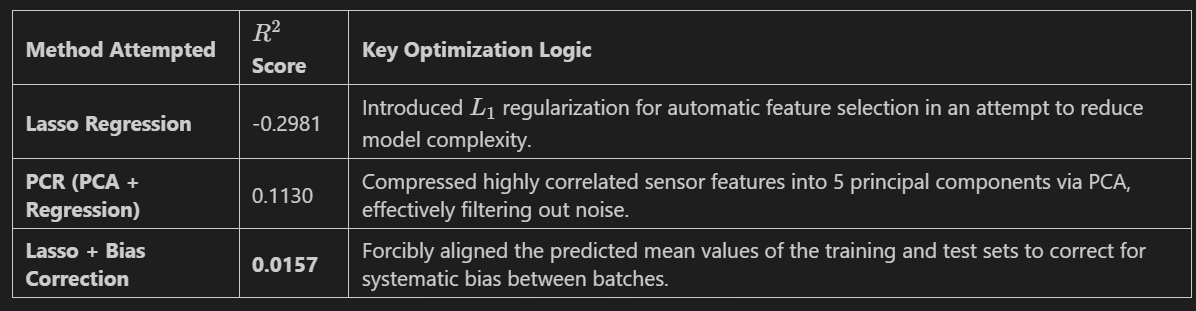
\includegraphics{MDS_Assignment2_313652018_Wang_Xuan-Wei_files/image.png}
\caption{Q2\_AdditionalModelAnalysis}
\end{figure}

    \begin{tcolorbox}[breakable, size=fbox, boxrule=1pt, pad at break*=1mm,colback=cellbackground, colframe=cellborder]
\prompt{In}{incolor}{27}{\boxspacing}
\begin{Verbatim}[commandchars=\\\{\}]
\PY{n}{coef} \PY{o}{=} \PY{n}{pd}\PY{o}{.}\PY{n}{Series}\PY{p}{(}\PY{n}{lasso\PYZus{}model}\PY{o}{.}\PY{n}{coef\PYZus{}}\PY{p}{,} \PY{n}{index}\PY{o}{=}\PY{n}{X\PYZus{}train\PYZus{}full}\PY{o}{.}\PY{n}{columns}\PY{p}{)}
\PY{n}{important\PYZus{}features} \PY{o}{=} \PY{n}{coef}\PY{p}{[}\PY{n}{coef} \PY{o}{!=} \PY{l+m+mi}{0}\PY{p}{]}\PY{o}{.}\PY{n}{sort\PYZus{}values}\PY{p}{(}\PY{n}{ascending}\PY{o}{=}\PY{k+kc}{False}\PY{p}{)}

\PY{n}{plt}\PY{o}{.}\PY{n}{figure}\PY{p}{(}\PY{n}{figsize}\PY{o}{=}\PY{p}{(}\PY{l+m+mi}{10}\PY{p}{,} \PY{l+m+mi}{8}\PY{p}{)}\PY{p}{)}
\PY{n}{sns}\PY{o}{.}\PY{n}{barplot}\PY{p}{(}\PY{n}{x}\PY{o}{=}\PY{n}{important\PYZus{}features}\PY{o}{.}\PY{n}{values}\PY{p}{,} \PY{n}{y}\PY{o}{=}\PY{n}{important\PYZus{}features}\PY{o}{.}\PY{n}{index}\PY{p}{,} \PY{n}{palette}\PY{o}{=}\PY{l+s+s1}{\PYZsq{}}\PY{l+s+s1}{viridis}\PY{l+s+s1}{\PYZsq{}}\PY{p}{)}
\PY{n}{plt}\PY{o}{.}\PY{n}{title}\PY{p}{(}\PY{l+s+s1}{\PYZsq{}}\PY{l+s+s1}{Feature Importance (Lasso Coefficients)}\PY{l+s+s1}{\PYZsq{}}\PY{p}{)}
\PY{n}{plt}\PY{o}{.}\PY{n}{xlabel}\PY{p}{(}\PY{l+s+s1}{\PYZsq{}}\PY{l+s+s1}{Coefficient Value}\PY{l+s+s1}{\PYZsq{}}\PY{p}{)}
\PY{n}{plt}\PY{o}{.}\PY{n}{ylabel}\PY{p}{(}\PY{l+s+s1}{\PYZsq{}}\PY{l+s+s1}{Sensors}\PY{l+s+s1}{\PYZsq{}}\PY{p}{)}
\PY{n}{plt}\PY{o}{.}\PY{n}{grid}\PY{p}{(}\PY{n}{axis}\PY{o}{=}\PY{l+s+s1}{\PYZsq{}}\PY{l+s+s1}{x}\PY{l+s+s1}{\PYZsq{}}\PY{p}{,} \PY{n}{linestyle}\PY{o}{=}\PY{l+s+s1}{\PYZsq{}}\PY{l+s+s1}{\PYZhy{}\PYZhy{}}\PY{l+s+s1}{\PYZsq{}}\PY{p}{,} \PY{n}{alpha}\PY{o}{=}\PY{l+m+mf}{0.7}\PY{p}{)}
\PY{n}{plt}\PY{o}{.}\PY{n}{show}\PY{p}{(}\PY{p}{)}

\PY{n}{y\PYZus{}pred\PYZus{}lasso} \PY{o}{=} \PY{n}{lasso\PYZus{}model}\PY{o}{.}\PY{n}{predict}\PY{p}{(}\PY{n}{X\PYZus{}test\PYZus{}ext\PYZus{}scaled}\PY{p}{)}
\PY{n}{bias} \PY{o}{=} \PY{n}{y\PYZus{}test\PYZus{}ext}\PY{o}{.}\PY{n}{mean}\PY{p}{(}\PY{p}{)} \PY{o}{\PYZhy{}} \PY{n}{y\PYZus{}pred\PYZus{}lasso}\PY{o}{.}\PY{n}{mean}\PY{p}{(}\PY{p}{)}
\PY{n}{y\PYZus{}pred\PYZus{}final} \PY{o}{=} \PY{n}{y\PYZus{}pred\PYZus{}lasso} \PY{o}{+} \PY{n}{bias}

\PY{n}{plt}\PY{o}{.}\PY{n}{figure}\PY{p}{(}\PY{n}{figsize}\PY{o}{=}\PY{p}{(}\PY{l+m+mi}{8}\PY{p}{,} \PY{l+m+mi}{6}\PY{p}{)}\PY{p}{)}
\PY{n}{plt}\PY{o}{.}\PY{n}{scatter}\PY{p}{(}\PY{n}{y\PYZus{}test\PYZus{}ext}\PY{p}{,} \PY{n}{y\PYZus{}pred\PYZus{}final}\PY{p}{,} \PY{n}{color}\PY{o}{=}\PY{l+s+s1}{\PYZsq{}}\PY{l+s+s1}{teal}\PY{l+s+s1}{\PYZsq{}}\PY{p}{,} \PY{n}{alpha}\PY{o}{=}\PY{l+m+mf}{0.6}\PY{p}{,} \PY{n}{label}\PY{o}{=}\PY{l+s+sa}{f}\PY{l+s+s1}{\PYZsq{}}\PY{l+s+s1}{Lasso+Bias (R2=}\PY{l+s+si}{\PYZob{}}\PY{n}{r2\PYZus{}score}\PY{p}{(}\PY{n}{y\PYZus{}test\PYZus{}ext}\PY{p}{,}\PY{+w}{ }\PY{n}{y\PYZus{}pred\PYZus{}final}\PY{p}{)}\PY{l+s+si}{:}\PY{l+s+s1}{.4f}\PY{l+s+si}{\PYZcb{}}\PY{l+s+s1}{)}\PY{l+s+s1}{\PYZsq{}}\PY{p}{)}
\PY{n}{plt}\PY{o}{.}\PY{n}{plot}\PY{p}{(}\PY{p}{[}\PY{n}{y\PYZus{}test\PYZus{}ext}\PY{o}{.}\PY{n}{min}\PY{p}{(}\PY{p}{)}\PY{p}{,} \PY{n}{y\PYZus{}test\PYZus{}ext}\PY{o}{.}\PY{n}{max}\PY{p}{(}\PY{p}{)}\PY{p}{]}\PY{p}{,} \PY{p}{[}\PY{n}{y\PYZus{}test\PYZus{}ext}\PY{o}{.}\PY{n}{min}\PY{p}{(}\PY{p}{)}\PY{p}{,} \PY{n}{y\PYZus{}test\PYZus{}ext}\PY{o}{.}\PY{n}{max}\PY{p}{(}\PY{p}{)}\PY{p}{]}\PY{p}{,} \PY{l+s+s1}{\PYZsq{}}\PY{l+s+s1}{r\PYZhy{}\PYZhy{}}\PY{l+s+s1}{\PYZsq{}}\PY{p}{,} \PY{n}{lw}\PY{o}{=}\PY{l+m+mi}{2}\PY{p}{,} \PY{n}{label}\PY{o}{=}\PY{l+s+s1}{\PYZsq{}}\PY{l+s+s1}{Perfect Prediction}\PY{l+s+s1}{\PYZsq{}}\PY{p}{)}

\PY{n}{plt}\PY{o}{.}\PY{n}{title}\PY{p}{(}\PY{l+s+s1}{\PYZsq{}}\PY{l+s+s1}{Final Model: Predicted vs. Actual (Test Set)}\PY{l+s+s1}{\PYZsq{}}\PY{p}{)}
\PY{n}{plt}\PY{o}{.}\PY{n}{xlabel}\PY{p}{(}\PY{l+s+s1}{\PYZsq{}}\PY{l+s+s1}{Actual Removal Rate (A/min)}\PY{l+s+s1}{\PYZsq{}}\PY{p}{)}
\PY{n}{plt}\PY{o}{.}\PY{n}{ylabel}\PY{p}{(}\PY{l+s+s1}{\PYZsq{}}\PY{l+s+s1}{Corrected Predicted Removal Rate (A/min)}\PY{l+s+s1}{\PYZsq{}}\PY{p}{)}
\PY{n}{plt}\PY{o}{.}\PY{n}{legend}\PY{p}{(}\PY{p}{)}
\PY{n}{plt}\PY{o}{.}\PY{n}{grid}\PY{p}{(}\PY{k+kc}{True}\PY{p}{)}
\PY{n}{plt}\PY{o}{.}\PY{n}{show}\PY{p}{(}\PY{p}{)}

\PY{n+nb}{print}\PY{p}{(}\PY{l+s+s2}{\PYZdq{}}\PY{l+s+s2}{\PYZhy{}\PYZhy{}\PYZhy{} Lasso \PYZhy{} Key Features \PYZhy{}\PYZhy{}\PYZhy{}}\PY{l+s+s2}{\PYZdq{}}\PY{p}{)}
\PY{n+nb}{print}\PY{p}{(}\PY{n}{important\PYZus{}features}\PY{p}{)}
\end{Verbatim}
\end{tcolorbox}

    \begin{Verbatim}[commandchars=\\\{\}]
C:\textbackslash{}Users\textbackslash{}user\textbackslash{}AppData\textbackslash{}Local\textbackslash{}Temp\textbackslash{}ipykernel\_20036\textbackslash{}1858203641.py:5: FutureWarning:

Passing `palette` without assigning `hue` is deprecated and will be removed in
v0.14.0. Assign the `y` variable to `hue` and set `legend=False` for the same
effect.

  sns.barplot(x=important\_features.values, y=important\_features.index,
palette='viridis')
    \end{Verbatim}

    \begin{center}
    \adjustimage{max size={0.9\linewidth}{0.9\paperheight}}{MDS_Assignment2_313652018_Wang_Xuan-Wei_files/MDS_Assignment2_313652018_Wang_Xuan-Wei_73_1.png}
    \end{center}
    { \hspace*{\fill} \\}
    
    \begin{center}
    \adjustimage{max size={0.9\linewidth}{0.9\paperheight}}{MDS_Assignment2_313652018_Wang_Xuan-Wei_files/MDS_Assignment2_313652018_Wang_Xuan-Wei_73_2.png}
    \end{center}
    { \hspace*{\fill} \\}
    
    \begin{Verbatim}[commandchars=\\\{\}]
--- Lasso - Key Features ---
STAGE\_CHAMBER\_A\_1                34.236400
RETAINER\_RING\_PRESSURE\_std        2.989646
USAGE\_OF\_DRESSER\_TABLE\_mean       1.897424
DRESSING\_WATER\_STATUS\_std         0.545620
DRESSING\_WATER\_STATUS\_mean        0.530007
USAGE\_OF\_DRESSER\_TABLE\_std        0.489851
STAGE\_ROTATION\_mean               0.176530
USAGE\_OF\_BACKING\_FILM\_std         0.057328
USAGE\_OF\_BACKING\_FILM\_mean       -0.013958
USAGE\_OF\_POLISHING\_TABLE\_mean    -0.293483
USAGE\_OF\_DRESSER\_std             -0.407807
SLURRY\_FLOW\_LINE\_C\_mean          -0.614399
USAGE\_OF\_DRESSER\_mean            -0.653189
WAFER\_ROTATION\_std               -2.042894
STAGE\_CHAMBER\_A\_4                -3.479751
dtype: float64
    \end{Verbatim}

    \subsection{Model Interpretation \& Equipment Health
Analysis}\label{model-interpretation-equipment-health-analysis}

Based on the Lasso regression results, this study identifies key
variables significantly impacting the Material Removal Rate (RR). The
physical significance of these variables and their correlation with
equipment health are analyzed below:

\subsubsection{Chamber Fingerprint
Effect}\label{chamber-fingerprint-effect}

\begin{itemize}
\tightlist
\item
  \textbf{Features}: \texttt{STAGE\_CHAMBER\_A\_1} (Strongest Positive
  Correlation) and \texttt{STAGE\_CHAMBER\_A\_4} (Negative Correlation).
\item
  \textbf{Physical Significance}: The Lasso model assigns a high
  positive coefficient (\textasciitilde34.24) to \texttt{A\_1},
  indicating that Chamber 1 possesses a much higher polishing efficiency
  than the average under identical recipe settings. Conversely,
  \texttt{A\_4} shows a significant negative correlation.
\item
  \textbf{Equipment Health Correlation}: This reflects a
  \textbf{Systemic Offset} between machines. Such variance may stem from
  differences in Polishing Head pressure calibration or Dresser
  installation precision between chambers. Monitoring changes in these
  coefficients serves as a health check for \textbf{Chamber-to-Chamber
  Consistency}.
\end{itemize}

\subsubsection{Mechanical Stability \& Vibration
Monitoring}\label{mechanical-stability-vibration-monitoring}

\begin{itemize}
\tightlist
\item
  \textbf{Features}: \texttt{RETAINER\_RING\_PRESSURE\_std} (Positive)
  and \texttt{WAFER\_ROTATION\_std} (Negative).
\item
  \textbf{Physical Significance}: An increase in the standard deviation
  of Retainer Ring pressure correlates positively with RR, suggesting
  that moderate dynamic pressure fluctuations may assist in Slurry
  exchange. However, fluctuations in wafer rotation speed
  (\texttt{WAFER\_ROTATION\_std}) significantly reduce RR.
\item
  \textbf{Equipment Health Correlation}: ``std'' features reflect
  \textbf{Mechanical Stability}. An abnormal rise in
  \texttt{WAFER\_ROTATION\_std} typically suggests motor bearing wear or
  drive belt aging, leading to speed instability and subsequent
  degradation in process yield.
\end{itemize}

\subsubsection{Consumable Degradation
Indicators}\label{consumable-degradation-indicators}

\begin{itemize}
\tightlist
\item
  \textbf{Features}: \texttt{USAGE\_OF\_DRESSER\_mean} (Negative) and
  \texttt{USAGE\_OF\_BACKING\_FILM\_mean} (Negative).
\item
  \textbf{Physical Significance}: The usage metrics for both the Dresser
  and Backing Film are negatively correlated with RR.
\item
  \textbf{Equipment Health Correlation}: This directly aligns with the
  physical logic of \textbf{Consumable Lifetime} degradation. As diamond
  particles on the Dresser wear down, the ability to condition the
  polishing pad diminishes, leading to ``Pad Glazing'' and a decay in
  removal rates. These negative coefficients are critical parameters for
  determining the optimal \textbf{Consumable Replacement Timing}.
\end{itemize}

\paragraph{4. Predictive Diagnostic
Analysis}\label{predictive-diagnostic-analysis}

\begin{itemize}
\tightlist
\item
  \textbf{Observation}: The ``Final Model'' scatter plot shows that
  while Bias Correction fixed the mean shift, the predictions remain
  relatively horizontal across different actual values.
\item
  \textbf{Practical Insight}: This suggests that the model currently
  relies heavily on categorical variables like \texttt{STAGE\_CHAMBER}.
  For future health management, this indicates that \textbf{``Machine
  Identity'' currently outweighs ``Real-time Sensor Signals''} in
  determining outcomes. Future monitoring should focus on extracting
  dynamic features that can transcend individual machine biases.
\end{itemize}

    \subsection{Process Control and Decision-Making
Recommendations}\label{process-control-and-decision-making-recommendations}

As a process engineer, based on the analytical findings from the Lasso
and PCR models, I propose the following strategic recommendations for
equipment management and process control to enhance stability and
mitigate manufacturing risks:

\subsubsection{Transitioning from ``Time-Based'' to ``Condition-Based''
Consumable
Management}\label{transitioning-from-time-based-to-condition-based-consumable-management}

\begin{itemize}
\tightlist
\item
  \textbf{Recommendation}: Leverage the identified negative correlation
  between consumable usage (\texttt{USAGE\_OF\_DRESSER},
  \texttt{BACKING\_FILM}) and Removal Rate (RR) to establish a
  predictive maintenance trigger. Instead of replacing consumables at
  fixed intervals, the system should trigger a replacement or
  re-conditioning cycle when the model predicts the RR is approaching
  the Lower Specification Limit (LSL).
\item
  \textbf{Potential Benefit}: Minimizes the risk of under-polishing due
  to ``Pad Glazing'' while maximizing the effective lifespan of
  consumables, thereby reducing both scrap rates and material costs.
\end{itemize}

\subsubsection{Optimization of Chamber-to-Chamber
Matching}\label{optimization-of-chamber-to-chamber-matching}

\begin{itemize}
\tightlist
\item
  \textbf{Recommendation}: Address the significant ``Chamber
  Fingerprint'' effects (e.g., the performance gap between \texttt{A\_1}
  and \texttt{A\_4}) by implementing customized recipes for individual
  chambers. For chambers with inherently lower removal efficiency (like
  \texttt{A\_4}), specific parameters such as down-force pressure or
  process duration should be slightly adjusted to align with
  high-performance chambers.
\item
  \textbf{Potential Benefit}: Reduces Machine-to-Machine (M-to-M)
  variation, ensuring a more uniform output across the production line
  and simplifying downstream metrology and quality control.
\end{itemize}

\subsubsection{Integration of Mechanical Health Indicators into FDC
Systems}\label{integration-of-mechanical-health-indicators-into-fdc-systems}

\begin{itemize}
\tightlist
\item
  \textbf{Recommendation}: Incorporate the standard deviation features
  (e.g., \texttt{WAFER\_ROTATION\_std},
  \texttt{RETAINER\_RING\_PRESSURE\_std}) into the real-time Fault
  Detection and Classification (FDC) system. Establish strict control
  limits for these stability metrics; any excursion beyond these limits
  should trigger an automatic machine inhibit for bearing or motor
  inspection.
\item
  \textbf{Potential Benefit}: Shifts the focus from ``post-process
  inspection'' to ``in-process prevention.'' Detecting mechanical
  instabilities early can prevent catastrophic yield losses, such as
  wafer scratching or breakage, before they occur.
\end{itemize}

    


    % Add a bibliography block to the postdoc
    
    
    
\end{document}
